 \documentclass[11pt, a4paper, spanish]{article}
     
\usepackage{float}
\usepackage{wrapfig}
\usepackage{sidecap}
\usepackage{subcaption}

\usepackage[a4paper, margin=2.5cm, top=3.5cm, bottom=3.5cm]{geometry} % Define los márgenes
\usepackage{amsmath, amscd, amssymb, amsthm, latexsym, gensymb} % Paquetes matemáticos
\usepackage[spanish]{babel} % Traduce los paquetes a español
\usepackage{ dsfont } %para usar simbolo de Naturales
\usepackage[utf8]{inputenc} % Codificación UTF8
\usepackage{fancyhdr} % Encabezados y pies de página
    \pagestyle{fancyplain}
\usepackage{enumerate}
\usepackage{xspace}


%\usepackage[page, toc]{appendix} % Apéndices
%\usepackage[nottoc]{tocbibind} % Referencias en la TDC
\usepackage{scrextend} % Para usar addmargin
\usepackage{listings} % Código
    \lstdefinestyle{customcpp}{
        belowcaptionskip=1\baselineskip,
        breaklines=true,
        xleftmargin=3em,
        language=C++,
        basicstyle=\small\ttfamily
    }
\usepackage[onelanguage, spanish]{algorithm2e}
    % \NoCaptionOfAlgo
    \LinesNumbered\RestyleAlgo{ruled}\IncMargin{1em}\DontPrintSemicolon\SetArgSty{}\SetCommentSty{textsf}\SetFuncSty{textsf}
    \SetKwProg{For}{para}{ hacer}{fin}
    \SetKwProg{Fn}{función}{:}{fin}
%\usepackage[pdflatex]{graphicx} % Imágenes
\usepackage[usenames,dvipsnames]{color} % Autoexplicativo
%\usepackage{caption} % Captions sin números
%\usepackage{multirow}
\usepackage{caratula} % Carátula del DC
\usepackage{url}
\usepackage{tikz}

%para las flechas de las aristas
\tikzset{
every picture/.append style={
  execute at begin picture={\deactivatequoting},
  execute at end picture={\activatequoting}
  }
}




\usepackage{xspace}
\usepackage{xargs}
\usepackage{ifthen}



\let\NombreFuncion=\textsc
\let\TipoVariable=\texttt
\let\tipo=\texttt
\let\ModificadorArgumento=\textbf
\newcommand{\res}{$res$\xspace}
\newcommand{\tab}{\hspace*{7mm}}


\newcommandx{\TipoFuncion}[3]{%
  \NombreFuncion{#1}(#2) \ifx#3\empty\else $\to$ \res\,: \TipoVariable{#3}\fi%
}

\newcommand{\In}[2]{\ModificadorArgumento{in} \ensuremath{#1}\,: \TipoVariable{#2}\xspace}
\newcommand{\Out}[2]{\ModificadorArgumento{out} \ensuremath{#1}\,: \TipoVariable{#2}\xspace}
\newcommand{\Inout}[2]{\ModificadorArgumento{in/out} \ensuremath{#1}\,: \TipoVariable{#2}\xspace}
\newcommand{\Aplicar}[2]{\NombreFuncion{#1}(#2)}


%%%%%%%%%%%%%%%%%%%%%%%%%%%%%%%% Macros de diseño propias %

\usepackage{scrextend} % Para poder indentar bloques

\newenvironment{paramFormales}{
  \textbf{par\'ametros formales}
  \vspace{-0.5em}
  \list{}{\leftmargin8em \topsep0.2em \itemsep0.25em \labelsep2em}
}{
  \endlist 
}

\newcommand{\servUsados}[1]{\textbf{Servicios usados:} #1 \\}

\newcommand{\paramGeneros}[1]{\item[\textbf{g\'eneros}] #1}

\newcommand{\paramFuncion}[1]{\item[\textbf{funci\'on}] \parbox[t]{\textwidth-2\parindent-1.7cm}{#1}}

\newcommand{\seExplicaCon}[1]{\parbox{3cm}{\textbf{se explica con}:} \tadNombre{#1}}

\newcommand{\generos}[1]{\parbox{3cm}{\textbf{g\'eneros}:} #1}

\newcommand{\campoTupla}[2]{\textrm{\textit{#1:}} \TipoVariable{#2}}

%\usepackage[noresetcount]{algorithm2e}
%\usepackage{float}

\NoCaptionOfAlgo\LinesNumbered\RestyleAlgo{ruled}\IncMargin{1em}\DontPrintSemicolon\SetArgSty{}\SetCommentSty{textsf}\SetFuncSty{textsf}

\newenvironment{algoritmo}[3]{
  \setcounter{AlgoLine}{0}
  \begin{algorithm}[H]\SetAlgoLined\SetAlgoLongEnd
  \caption{\TipoFuncion{#1}{#2}{#3}}
}{
  \end{algorithm}
  \vspace{0em}
}

\newenvironment{contAlgoritmo}[1]{
  \begin{algorithm}[H]\SetAlgoLined\SetAlgoLongEnd
  \caption{\NombreFuncion{#1} \emph{(cont.)}}
}{
  \end{algorithm}
}

\newcommand{\datosAlgoritmo}[5]{
  \ifx#1\empty\else \textbf{Descripci\'on:} #1

  \fi \ifx#2\empty\else\textbf{Pre} $\equiv$ \{#2\}

  \fi \ifx#3\empty\else\textbf{Post} $\equiv$ \{#3\}

  \fi \textbf{Complejidad:} #4 

  \ifx#5\empty\else\textbf{Justificaci\'on:} #5 \fi \vspace{1em}
}

\SetKwComment{com}{ $\triangleright$ }{}
\def\new{\textbf{\&}}
\def\NULL{\textrm{NULL}}


% Encabezado
\lhead{Algoritmos y estructuras de datos III}
\rhead{Trabajo Práctico Nº 3}
% Pie de pagina
\renewcommand{\footrulewidth}{0.4pt}
% \lfoot{FCEN}
% \rfoot{UBA}


\begin{document}

\lstset{language=c++}
\lstdefinestyle{customc}{
  belowcaptionskip=1\baselineskip,
  breaklines=true,
  frame=L,
  xleftmargin=\parindent,
  language=C,
  showstringspaces=false,
  basicstyle=\footnotesize\ttfamily,
  keywordstyle=\bfseries\color{green!40!black},
  commentstyle=\itshape\color{purple!40!black},
  identifierstyle=\color{blue},
  stringstyle=\color{orange},
}

% Datos de carátula
\materia{Algoritmos y estructuras de datos III}
\titulo{Trabajo Práctico Nº 3}
\fecha{Primer cuatrimestre de 2016}

\integrante{Goldstein, Brian}{027/14}{brai.goldstein@gmail.com}
\integrante{Martínez, Manuela}{160/14}{martinez.manuela.22@gmail.com}
\integrante{Rabinowicz, Lucía}{105/14}{lu.rabinowicz@gmail.com}
\integrante{Ginsberg, Mario Ezequiel}{145/14}{ezequielginsberg@gmail.com}


% Carátula
\maketitle
\newpage


% Índice
\tableofcontents
\clearpage

% Contenido
\section{Ejercicio 1}

\noindent En este trabajo se busca hallar, dados dos grafos simples $G_{1}$=($V_{1}$, $E_{1}$) y $G_{2}$=($V_{2}$, $E_{2}$), el máximo subgrafo común o MCS.\\
El máximo subgrafo común consiste en encontrar un grafo $H$=($V_{H}$, $E_{H}$) isomorfo tanto a un subgrafo de  $G_{1}$ como a un subgrafo de $G_{2}$ que maximice $\#E_{H}$.\\
El problema de grafos planteado en el paper es muy similar al de MCS (máximo subgrafo común) pero con la diferencia de que al plantearse un problema químico, el grafo representa una molécula, por lo que cada uno de sus nodos tiene un nombre asociado. En el caso del problema a resolver por Doc, los nodos son todos iguales (no tienen label). Para poder reutilizar algún algoritmo que resuelve el problema del paper, se puede tomar como parámetro de entrada el grafo en cuestión en el cual todos los nodos tienen la misma etiqueta.\\
En la química muchas veces es útil encontrar subesctructuras comunes entre moléculas, que se pueden encontrar a partir de representar una molécula con sus respectivos enlaces mediante un vértice por átomo y una arista por enlace, y aplicar algún algoritmo que resuelva MCS.\\
Aplicaciones en concreto pueden ser, por ejemplo, reducir la cantidad de experimentos necesarios para entender la capacidad de ciertas moléculas de actuar como drogas, ya que dado dos moléculas estructuralmente similares suelen tener ``actividad'' similar (suelen hacer efectos similares). Por lo que si uno quisiese estudiar un conjunto grande de moléculas para encontrar sus propiedades activas, en principio no sería necesario experimentar con todas, sino que podría agruparlas de a grupos con MCS lo suficientemente grandes y a partir de ahí estudiar las propiedades de cada grupo experimentando con unos pocos representantes por grupo.
\clearpage
\section{Ejercicio 2}

\subsection{Introducción}

\noindent Este ejercicio consiste en resolver el problema que busca el MCS entre dos grafos con un algoritmo exacto. Este es un problema de tipo NP-completo. Más adelante calcularemos la complejidad exacta y luego desarrollaremos diferentes heurísticas basadas en metaheurísticas polinomiales, que a pesar de que no aseguran un resultado exacto, a veces pueden resultar convenientes ya que la diferencia de tiempos es muy notable.

\subsection{Implementación}

\noindent El algoritmo recibe dos grafos y se quiere hallar al máximo subgrafo común entre ellos. Sea $G1$ el grafo que tiene la menor cantidad de nodos y $G2$ el otro grafo. Si ambos tienen igual cantidad de nodos es indistinto cuál es $G1$ y cuál es $G2$.\\

\noindent El algoritmo funciona de la siguiente forma: 
\begin{itemize}
\item Primero notemos que el grafo solución va a tener la misma cantidad de nodos que el grafo $G1$. Esto se encuentra justificado en el $Lema 1$.
\item Ahora se quiere maximizar la cantidad de aristas que podemos encontrar entre los dos grafos, tomando como cantidad de nodos, la cantidad de nodos de $G1$. \\
Para ello utilizamos un vector $mapeo$ en el cual cada posición representa un nodo del grafo $G1$ (la posición $i$ representa el nodo del subgrafo común al cual mapeamos el nodo $i$ del grafo $G1$, con 0 $\leq$ $i$ $<$ $cantidad$ $de$ $nodos$ $de$ $G1$) y el valor de esa posición será el nodo que se corresponde con éste en $G2$ (el nodo $i$ de $G1$ se corresponde con el nodo $vector[i]$ de $G2$).
\begin{figure}[H]
\centering
\begin{subfigure}[h]{0.2\textwidth}
  \begin{tikzpicture}[scale= 0.6]
  \node[draw,circle,thick](0) at (0,0){0}; \\
   \node[draw,circle,thick](1) at (0,2){1}; \\
   \node[draw,circle,thick](2) at (2,0){2}; \\
  % \draw [thick,->] (a) to [out=120,in=180] (b);
   \draw [thick] (0) -- (1);
   \draw [thick] (1) -- (2);
   \draw [thick] (0) -- (2);
  \end{tikzpicture}
\caption{$G1$}
 \end{subfigure}
\begin{subfigure}[h]{0.2\textwidth}
  \begin{tikzpicture}[scale= 0.6]
  \node[draw,circle,thick](0) at (-2,6){0}; \\
   \node[draw,circle,thick](1) at (0,6){1}; \\
   \node[draw,circle,thick](2) at (0,4){2}; \\
    \node[draw,circle,thick](3) at (0,2){3}; \\
   \node[draw,circle,thick](4) at (0,0){4}; \\
   \node[draw,circle,thick](5) at (2,0){5}; \\

  % \draw [thick,->] (a) to [out=120,in=180] (b);
   \draw [thick] (0) -- (1);
   \draw [thick] (1) -- (2);
   \draw [thick] (2) -- (3); 
   \draw [thick] (3) -- (4);
   \draw [thick] (3) -- (5);
   \draw [thick] (4) -- (5);
  \end{tikzpicture}
\caption{$G2$}
\end{subfigure}
\end{figure}

\begin{figure}[H]
\centering
\begin{subfigure}[H]{0.4\textwidth}

\begin{table}[H]
\centering Mapeo
\label{my-label}
\begin{tabular}{ccc}
\hline
\multicolumn{1}{|c|}{\textbf{3}} & \multicolumn{1}{c|}{\textbf{4}} & \multicolumn{1}{c|}{\textbf{5}} \\ \hline
0                                & 1                               & 2                              
\end{tabular}
\end{table}
\end{subfigure}
\begin{subfigure}[H]{0.4\textwidth}


\begin{table}[H]
\centering
\label{my-label}
\begin{tabular}{clc}
\textbf{Aristas de $G1$} & \multicolumn{1}{c}{\textbf{}}         & \textbf{Aristas de $G2$} \\
(0,1)                  & $\leftrightarrow$ & (3,4)                  \\
(1,2)                  & $\leftrightarrow$                    & (4,5)                  \\
(2,0)                  & $\leftrightarrow$                     & (5,3)                 
\end{tabular}
\end{table}

\end{subfigure}
\caption{Ejemplo de mapeo}
\end{figure}


\item Luego comparamos la cantidad de aristas que se obtienen en cada mapeo posible, y nos quedamos con el que más tenga. 
\end{itemize}

\subsubsection*{Lema 1}
\noindent Sea $G1$ y $G2$ dos grafos donde $G1$ es el que tiene menor cantidad de nodos. Sea $G'$ un subgrafo común con la mayor cantidad de aristas posibles, y si hay más de uno entonces tomamos uno que tenga la mayor cantidad de vértices posibles, entonces $G'$ tiene la misma cantidad de nodos que $G1$. \\
$\mathbf{Demostraci\acute{o}n:}$ \\
\noindent Sea $G'$ el grafo definido en el enunciado del lema. Supongamos que $G'$ tiene menor cantidad de nodos que $G1$. Entonces si agrego un nodo más a $G'$ sin conectarle aristas sigue siendo subgrafo de $G1$ y por lo tanto de $G2$ también ya que $G2$ tiene mayor o igual cantidad de nodos que $G1$. Entonces $G'$ no era máximo en nodos. Absurdo. El absurdo viene de suponer que $G'$ puede tener menos nodos que $G1$. \\
Supongamos ahora que $G'$ tiene mayor cantidad de nodos que $G1$. Entonces $G'$ no es subgrafo de $G1$ ya que una de las condiciones para ser subgrafo es que el conjunto de nodos de $G'$ tiene que estar incluido en el de $G1$. Absurdo. El absurdo viene de suponer que $G'$ puede tener más nodos que $G1$.\\
Entonces como $G'$ no puede tener ni mayor ni menor cantidad de nodos que $G1$, entonces $G'$ tiene igual cantidad de nodos que $G1$. A los fines de este trabajo práctico escribiremos soluciones que encuentren subgrafos comunes que sean máximos en aristas y que tengan la misma cantidad de nodos que $G1$.\\


\begin{algoritmo}{MCS}{vector(int) mapeo, vector(vector(int)) grafoChico, vector(vector(int)) GrafoGrande }{void}

	\If(\com*{en maximaCantidadDeAristasPosibles se tiene la cantidad de aristas del grafoChico, el MCS no puede superar esta cantidad. Esta es la poda, ya que corta el algoritmo si llega a un resultado insuperable por mas de que no se hayan recorrido todos los mapeos posibles.}){CantidadAristasMejorSolucionHastaElMomento == maximaCantidadDeAristasPosibles}{
return \;
	}
	\For{(cadaMapeoPosible)}{

    	\If{la nueva solución es mejor que la que tengo guardada en CantidadAristasMejorSolucionHastaElMomento}{ 
    		aristasMejorSolucion = aristasDeLaNuevaSolución
    		CantidadAristasMejorSolucionHastaElMomento = CantidadDeAristasDeLaNuevaSolución
   		}
    MCS(mapeo,grafoChico,grafoGrande);
    }
\end{algoritmo}



\subsection{Complejidad}
Para calcular la complejidad de este algoritmo primero analizaremos la complejidad del mismo sin tener en cuenta la poda y luego verificaremos que la poda no empeora la complejidad del mismo.\\
La notación a utilizar será correspondiente a la utilizada anteriormente: los grafos serán $G1$ y $G2$ donde 
$\# V(G1) = n_1$, 
$\# A(G1) = m_1$ y 
$\# V(G2) = n_2$, 
$ \# A(G2) = m_1$ 
con $n_1 \leq n_2$.\\
Analizaremos entonces la complejidad del algoritmo despreciando la poda. Observamos para esto que el algoritmo se resume a: 
\begin{itemize}
	\item Recibir los parámetros de entrada.
	\item Aplicar la función MCS.
    \item Mostrar el resultado%, es decir, que la complejidad del algoritmo se vera en esta función.
\end{itemize}

Con esta observación podemos asegurar que la complejidad total del algoritmo estará dada por la cantidad de veces que se ejecuta la función $MCS(..)$, multiplicado por la complejidad de cada ejecución , es decir, la complejidad de la función en cada llamado multiplicado por la cantidad de llamadas.\\
Distinguimos que la complejidad de la ejecución de la función $MCS(..)$ depende si se la esta llamando con un mapeo (el vector mapeo) completo o uno incompleto, es decir, si el vector tiene el tamaño $n_1$ o si es mas chico. Analizaremos ambos casos por separado:

\begin{enumerate}[(a)]
  
\item Si se la está llamando con un mapeo completo, el algoritmo tarda $\mathcal{O}((n_1 + m_1)*m_2)$ como cota pues es lo que se tarda en recorrer G1 (y a la vez el vector ``mapeo'') y para cada nodo allí preguntar en $\mathcal{O}(m_2)$ qué aristas tienen en común con un vértice particular de G2 (dicho vértice lo determina ``mapeo''; observemos que si bien $G2$ tarda $\mathcal{O}(n_2+m_2)$ en recorrerse, al ya tener el índice del nodo a consultar sólo se recorren sus vecinos, que son a lo sumo $m_2$ y no es necesario el $n_2$ dado que no se recorren todos los nodos, sino sólo el indicado por ``mapeo''). En esta complejidad quedan absorbidos también los costos de comparar con el mejor mapeo hasta el momento y los costos de copiarlo en caso de ser el ``nuevo mejor mapeo'', ya que éstos son subgrafos de $G1$ y $G2$ así que en particular recorrerlos costará $\mathcal{O}(n_1+m_1)$ por ser $G1$ el más chico de ambos grafos y esto queda absorbido en la complejidad dicha ($\mathcal{O}((n_1 + m_1)*m_2)$).\\
Si uno se permitiese ser menos preciso podría decir que es $\mathcal{O}((n_1+m_1)*n_2^2)$ ya que la cantidad de aristas posibles de $G2$ están limitadas por la cantidad de aristas de $ \# A(K_{n_2}) \in \mathcal{O}(n_2^2)$ (esto último es por propiedad enunciada en las teóricas y prácticas), y perdiendo aún más precisión, usando la misma propiedad podría simplificarse a $\mathcal{O}((n_1+n_1^2)*n_2^2) = \mathcal{O}(n_1^2*n_2^2)$ y por último, como $n_1 \leq n_2$ a $\mathcal{O}(n_2^4)$. Estas simplificaciones son útiles para tener un visión panorámica a gran escala de la complejidad, pero por precisión, en el desarrollo que sigue usaremos la complejidad más precisa de $\mathcal{O}((n_1 + m_1)*m_2)$.
\item Si en cambio se la está llamando con un vector de mapeo incompleto, es decir, de tamaño menor estricto a $n_1$, entonces se procede a mapear uno mas, lo que tiene complejidad $\mathcal{O}(n_1)$ ya que para mapear uno mas (digamos que se quiere mapear el nuevo vértice $v_1$ de $G1$ al vértice $v_j$ de $G2$), se debe recorrer el vector ``mapeo'' y chequear que no haya otro ya mapeado al $v_j$, y una vez que verifica esto, realizar un push$\_$back() en 'mapeo', que se puede hacer ya que el vector mapeo tiene tamaño a lo sumo $n_1 - 1$, pues sino hubiese entrado en la opción $(a)$. La complejidad en este caso (en todo $(b)$) es $\mathcal{O}(n_1)$ que es la complejidad de recorrer el vector para chequear no repetir e insertar uno atrás.\\
\end{enumerate}

\noindent Sabemos, entonces, que cada llamada a $MCS(..)$ tendrá complejidad $\mathcal{O}((n_1 + m_1)*m_2)$ si se la llama con un mapeo completo (por $(a)$) y $\mathcal{O}(n_1)$ si se la llama con un mapeo incompleto (por $(b)$).\\
A continuación analizaremos la cantidad de veces que es llamada la función con parámetros de tipo $(a)$ y cuántas veces es llamada la función con parámetros de tipo $(b)$\\
Contaremos la cantidad de veces que se llama a la función con parámetros del tipo (a) primero:

\begin{itemize}
\item Para estar en el caso (a), el vector ``mapeo'' debe estar completo en sus $n_1$ posiciones con números de $0$ a $n_2 - 1$ (que representan a los vértices correspondientes a $G2$) todos distintos entre sí.
\item Observemos cuántas formas hay de llenar el vector cumpliendo con las condiciones del ítem anterior:\\

\begin{itemize}
\item Para la primer posición (la de índice $0$) hay $n_2$ posibilidades.
\item Para la segunda posición (índice $1$) hay $n_2 - 1$ posibilidades (porque no puedo repetir).
\item Para la posición $i$, en general hay $n_2-i$ posibilidades.
\item Para la última posición (índice $n_1-1$) habrá $n_2-n_1+1$ posibilidades.
\end{itemize}

\item Entonces observamos que la cantidad total de veces que se llamará al caso (a) será:
$n_2 * (n_2-1)*.....(n_2-i)....(n_2-(n_1-1))$ $\leq n_2 * n_2 * n_2*...........*n_2 \leq n_2^{n_1}$
\end{itemize}

Veremos ahora la cantidad de veces que se llama a la función con parámetros de tipo (b). Observemos que éstos son los pasos previos a cada construcción del tipo (a). En un principio hay una primer llamada de tipo (b) la cual realiza $n_2$ (una por cada número que es posible poner del 1 al $n_2$) llamadas, que a su vez realizan $n_2-1$ llamadas cada y así sucesivamente hasta que eventualmente se llegan a los casos tipo (a) y termina.\\
Esta sucesión de llamadas podría entenderse con el siguiente árbol:
    \begin{figure}[H]
      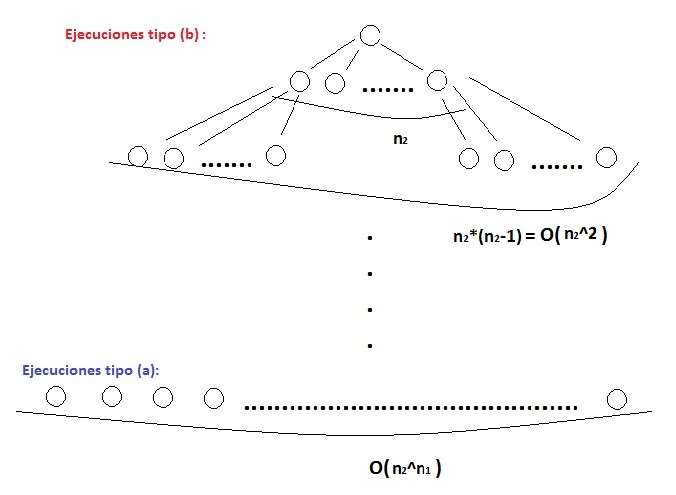
\includegraphics[height=10cm]{graficos/arbolesTipoAyB.jpg}
       \caption{Árbol de llamadas a MCS}
	\end{figure}
Se puede observar que es un árbol ``$n_2-ario$'' (las comillas están pues no es $n_2-ario$ ya que en cada nivel se baja en 1 el grado de cada nodo, pero en términos de complejidad es la misma por la misma justificación que usamos para contar los tipo(a)) completo de altura $n_1$. Como ya habíamos observado, la cantidad de veces que se ejecuta como tipo (a) es $\mathcal{O}(n_2^{n_1})$, que es la cantidad de hojas, mientras que la cantidad de veces que se ejecute como tipo (b) será la cantidad de nodos internos de éste árbol, que es orden de la cantidad de nodos de un $n_2-ario$ completo de $n_1 - 1$ de altura, que puede acotarse por $\mathcal{O}(n_2^{n_1})$.\\

Ya sabemos que se llaman $\mathcal{O}(n_2^{n_1})$ tanto a las ejecuciones tipo (a) como a las tipo (b), y además sabemos que las tipo (a) tiene complejidad $\mathcal{O}((n_1 + m_1)*m_2)$ mientras que las tipo (b) $\mathcal{O}(n_1)$. \\
Concluimos entonces que la complejidad total del algoritmo será $\mathcal{O}(n_2^{n_1}*((n_1 + m_1)*m_2)+n_2^{n_1}*n_1) = \mathcal{O}(n_2^{n_1}*(n_1 + m_1)*m_2) $.
\\ \\
Sólo quedaría ver que la poda no empeora esta complejidad, y no lo hace pues sólo realiza operaciones $\mathcal{O}(1)$ y su código esta comprendido dentro de las ejecuciones tipo (a) y (b), por lo que no aporta a la complejidad total, ya que ese $\mathcal{O}(1)$ es absorbido por las complejidades de las ejecuciones (a) o (b).
 
\subsection{Experimentación}
\noindent El algoritmo toma dos grafos para calcular el máximo subgrafo común, entonces para tomar las mediciones y determinar el tiempo de cómputo de la heurística, generalmente, se modificarán únicamente las cantidades de nodos y aristas de uno de ellos. \\
Sea $n_1$ y $m_1$ la cantidad de nodos y aristas del grafo que se modificará para tomar las mediciones respectivamente, y $n_2$, $m_2$ la cantidad de nodos y aristas del grafo al que se le dejarán constantes las cantidades de nodos y aristas, aunque en cada caso podrán utilizarse grafos distintos por con la misma cantidad de vértices y de aristas.
    
\subsubsection*{Experimento 1}\;
\noindent  El objetivo de este experimento fue extraer conclusiones acerca de la variación en el tiempo de cómputo requerido por el algoritmo para distintos valores de $m_1$, con el fin de determinar su complejidad, dejando $n_1$ fijo. \\
\noindent Para ello se utiliza un generador de grafos que funciona de la siguiente manera: dada una cantidad de nodos y aristas, en cada paso crea una nueva arista con extremos válidos (es decir, entre 0 y la cantidad de nodos - 1) y que no este repetida (que no haya sido creada todavía).
     	
\subsubsection*{Datos de entrada}\;
   		\noindent Para correr el algoritmo con poda los valores de $m_1$ tomados fueron desde $0$ hasta $28$ de $2$ en $2$. Como es un algoritmo que resuelve un problema de tipo NP-completo no se pudieron utilizar valores grandes ya que el tiempo de ejecución es muy alto. El valor de $n_1$ fue $8$.\\
       Los valores de $n_2$ y $m_2$ fueron $8$ y $17$ respectivamente. Estos valores fueron elegidos de forma arbitraria teniendo en cuenta que no se pueden utilizar números muy altos por las razones explicadas anteriormente\\
        Para generar los grafos de forma aleatoria se utilizó el generador-grafo-rapido.cpp que se encuentra en la carpeta src y para correrlo se utilizó el exp1.sh que se encuentra en la carpeta exp/ejercicio2/exp1. \\
        Para el caso del que no tiene poda se corrió el algoritmo con los mismos valores de $n_1$, $m_1$, $n_2$ y $m_2$ que en el caso anterior y se utilizó el mismo generador de grafos aleatorios. Para correrlo se utilizó el exp1.sh que se encuentra en la carpeta exp/ejercicio2/exp1bis.\\
        Con el fin de acercarse a los valores reales y descartar posibles falsos resultados, se ejecuta la resolución del problema para cada una de los valores de $m_1$ siete veces considerando luego el promedio entre los valores obtenidos pero graficando también el desvío estándar (la cantidad de repeticiones a realizar fue elegida arbitrariamente).\; 

\subsubsection*{Resultados}\;

    \begin{figure}[H]
      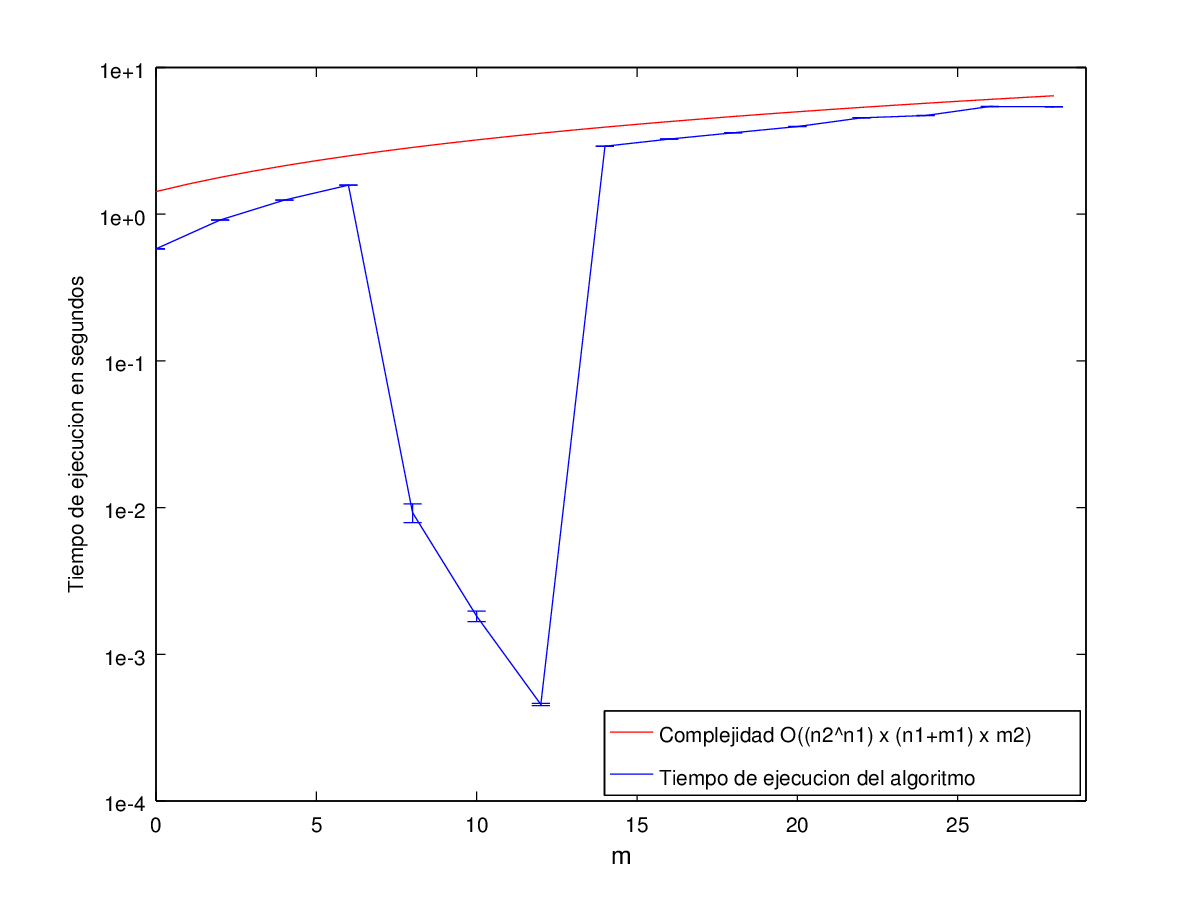
\includegraphics[height=10cm]{graficos/ejercicio2-exp1.png}
       \caption{Experimento 1}
	\end{figure}
    
    \begin{figure}[H]
      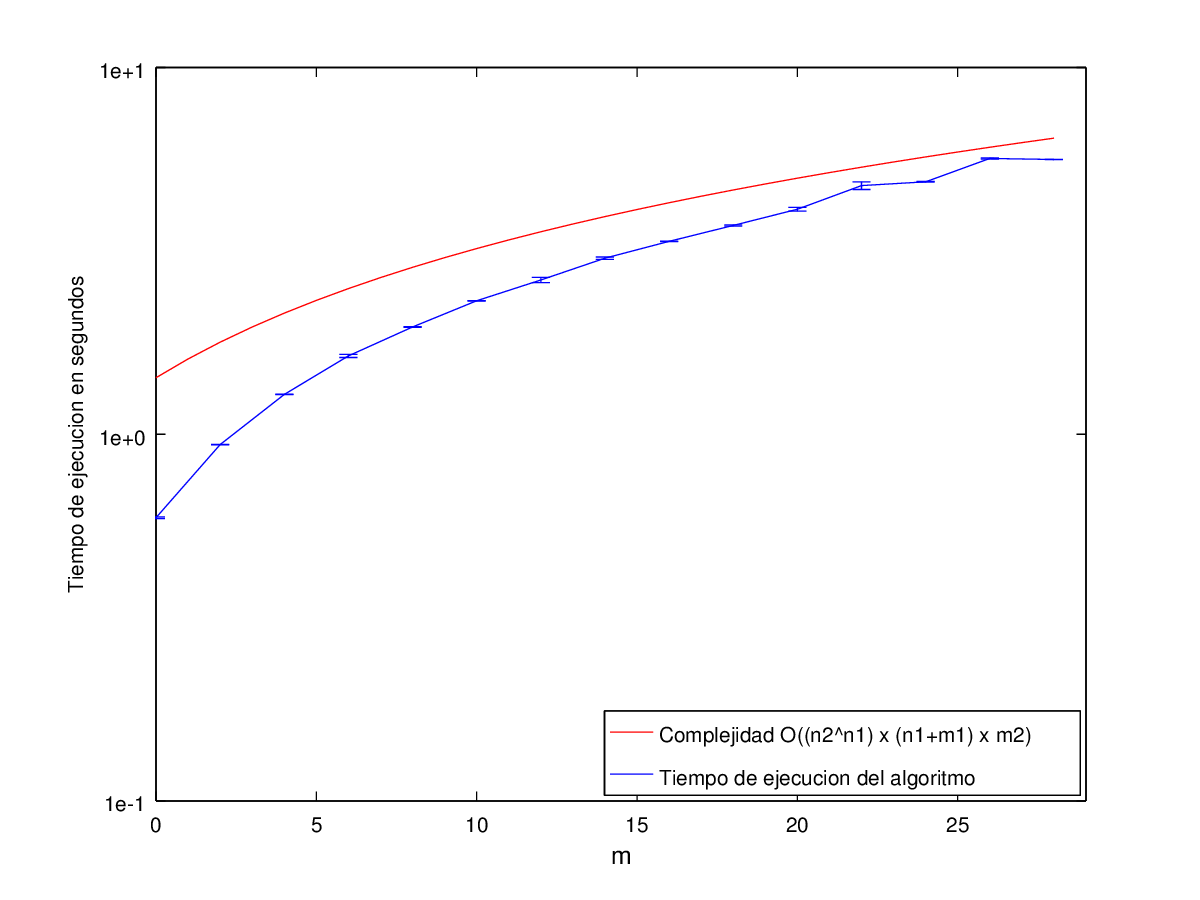
\includegraphics[height=10cm]{graficos/ejercicio2-exp1bis.png}
       \caption{Experimento 1 - Sin Poda}
	\end{figure}
\subsubsection*{Observaciones y Conclusiones}\;
En las dos figuras anteriores se puede observar como aumenta el tiempo en relación a lo esperado comportándose como el cálculo de complejidad lo sugiere. En la primer figura se puede observar como la poda efectivamente en algunos casos reduce el tiempo de ejecución (aunque no así la complejidad asintótica) en comparación con el algoritmo sin poda (segunda figura).\\
Concluimos que el experimento demuestra el comportamiento esperado en cuanto a variar la cantidad de aristas de G1 ($m_1$).\\

        
\subsubsection*{Experimento 2}\;
\noindent Este experimento es similar al anterior, pero ahora se va a variar la cantidad de nodos. Para ello, para cada cantidad de nodos se definirá una función para determinar la cantidad de aristas que tendrá el grafo. \\
\noindent Se tuvieron en cuenta 4 funciones, con el fin de que el grafo obtenido no sea siempre uno especial y de esta forma poder analizar diferentes casos.
        \begin{itemize}
        \item F1($n_1$) = $n_1$($n_1$-1))/2 = $m_1$ 
        \item F2($n_1$) = $n_1$-1 = $m_1$ 
        \item F3($n_1$) = 3$n_1$ = $m_1$ 
        \item F4($n_1$) = $n_1^{2}$/10 = $m_1$ 
		\end{itemize} 
Para generar los grafos con estas cantidades de aristas y nodos se utilizó el mismo generador que en el experimento anterior.

\subsubsection*{Datos de entrada}\;
\noindent Los valores de $n_1$ tomados fueron desde $1$ hasta $7$. Como es un algoritmo que resuelve un problema de tipo NP-completo no se pudieron utilizar valores grandes ya que el tiempo de ejecución es muy alto.\\
       Los valores de $n_2$ y $m_2$ fueron $10$ y $20$ respectivamente. Estos valores fueron elegidos de forma arbitraria teniendo en cuenta que no se pueden utilizar números muy altos por las razones explicadas anteriormente\\
        Para generar los grafos de forma aleatoria se utilizó el generador-grafo-rapido.cpp que se encuentra en la carpeta src y para correrlo se utilizó el exp2.sh que se encuentra en la carpeta exp/ejercicio2/exp2. \\
        Con el fin de acercarse a los valores reales y descartar posibles falsos resultados, se ejecuta la resolución del problema para cada una de los valores de $n_1$ cinco veces considerando luego el promedio entre los valores obtenidos pero graficando también el desvío estándar (la cantidad de repeticiones a realizar fue elegida arbitrariamente).\; 

\subsubsection*{Resultados}\;

    \begin{figure}[H]
      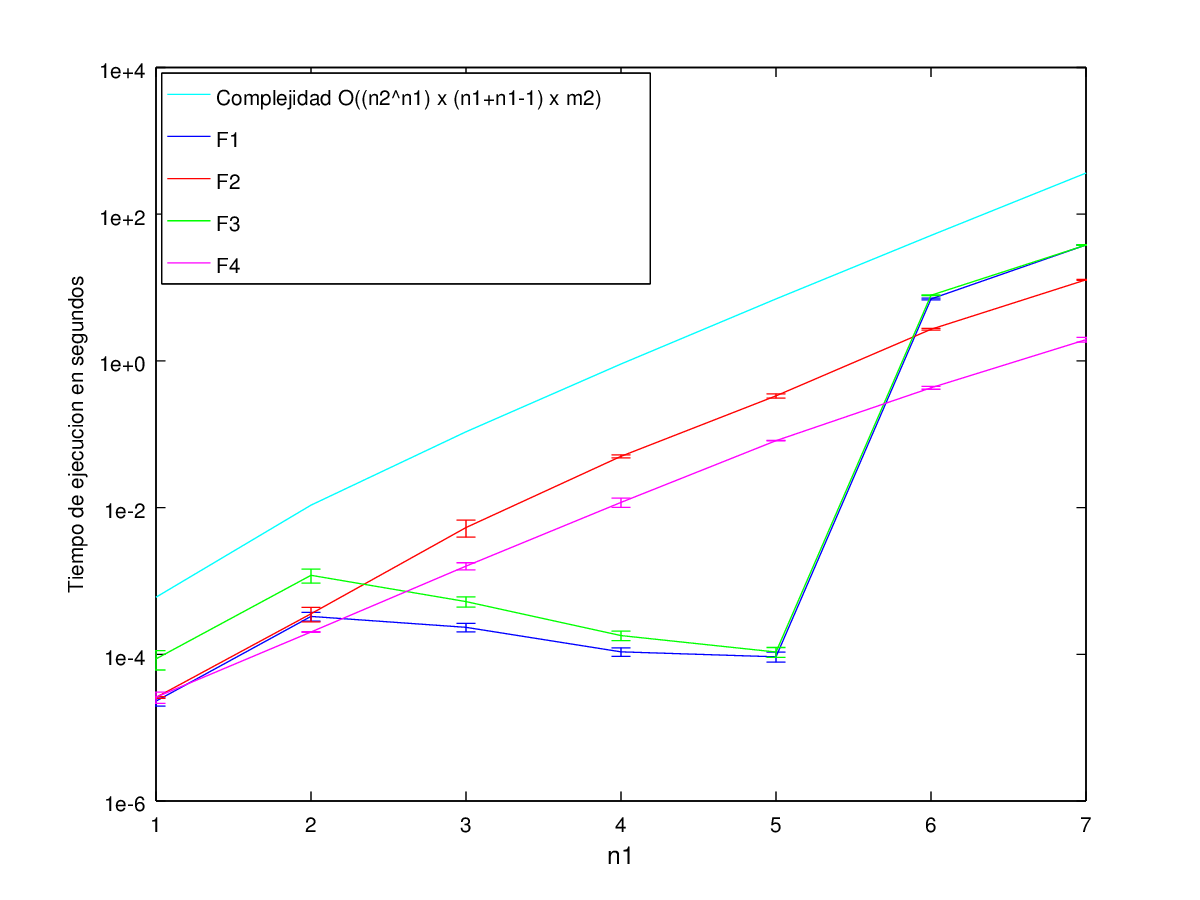
\includegraphics[height=10cm]{graficos/ejercicio2-exp2.png}
       \caption{Experimento 2}
	\end{figure}


\subsubsection*{Observaciones y Conclusiones}\;
 \noindent En la figura anterior puede observarse como en todos los casos el algoritmo parece respetar la complejidad propuesta cuando se varía la cantidad de nodos de G1 independientemente de su cantidad de aristas asociadas. Se puede observar también como en algunas circunstancias la poda reduce el tiempo de cómputo.\\
Ciertas simetrías en cuándo la poda es efectiva se pueden observar entre las diferentes F. Atribuimos esta coincidencia al echo de que los grafos a pesar de ser generados con distintas cantidades de aristas, son generados de forma similar.\\
Concluimos de este experimento que el tiempo de ejecución del algoritmo respeta la complejidad propuesta cuando se hace variar la cantidad de nodos del grafo G1.
    
\subsubsection*{Experimento 3}\; 
 \noindent El objetivo de este experimento fue extraer conclusiones acerca de la variación en el tiempo de cómputo requerido por el algoritmo para distintos valores de $m$ y $n$ variando los dos grafos al mismo tiempo pero siempre manteniendo $n_1$ igual a $n_2$ y $m_1$ igual a $m_2$. \\
Para generar los grafos con estas cantidades de aristas y nodos se utilizó el mismo generador que en el experimento anterior. 
        
\subsubsection*{Datos de entrada}\;
\noindent Los valores de $n$ tomados fueron desde $1$ hasta $8$. Como es un algoritmo que resuelve un problema de tipo NP-completo no se pudieron utilizar valores grandes ya que el tiempo de ejecución es muy alto. Para cada $n$ se utilizó $3 \times n$ como cantidad de aristas.\\
        Para generar los grafos de forma aleatoria se utilizó el generador-grafo-rapido.cpp que se encuentra en la carpeta src y para correrlo se utilizó el exp3.sh que se encuentra en la carpeta exp/ejercicio2/exp3. \\
        Con el fin de acercarse a los valores reales y descartar posibles falsos resultados, se ejecuta la resolución del problema para cada una de los valores de $n$ cinco veces considerando luego el promedio entre los valores obtenidos pero graficando también el desvío estándar (la cantidad de repeticiones a realizar fue elegida arbitrariamente).\; 
        
\subsubsection*{Resultados}\;

    \begin{figure}[H]
      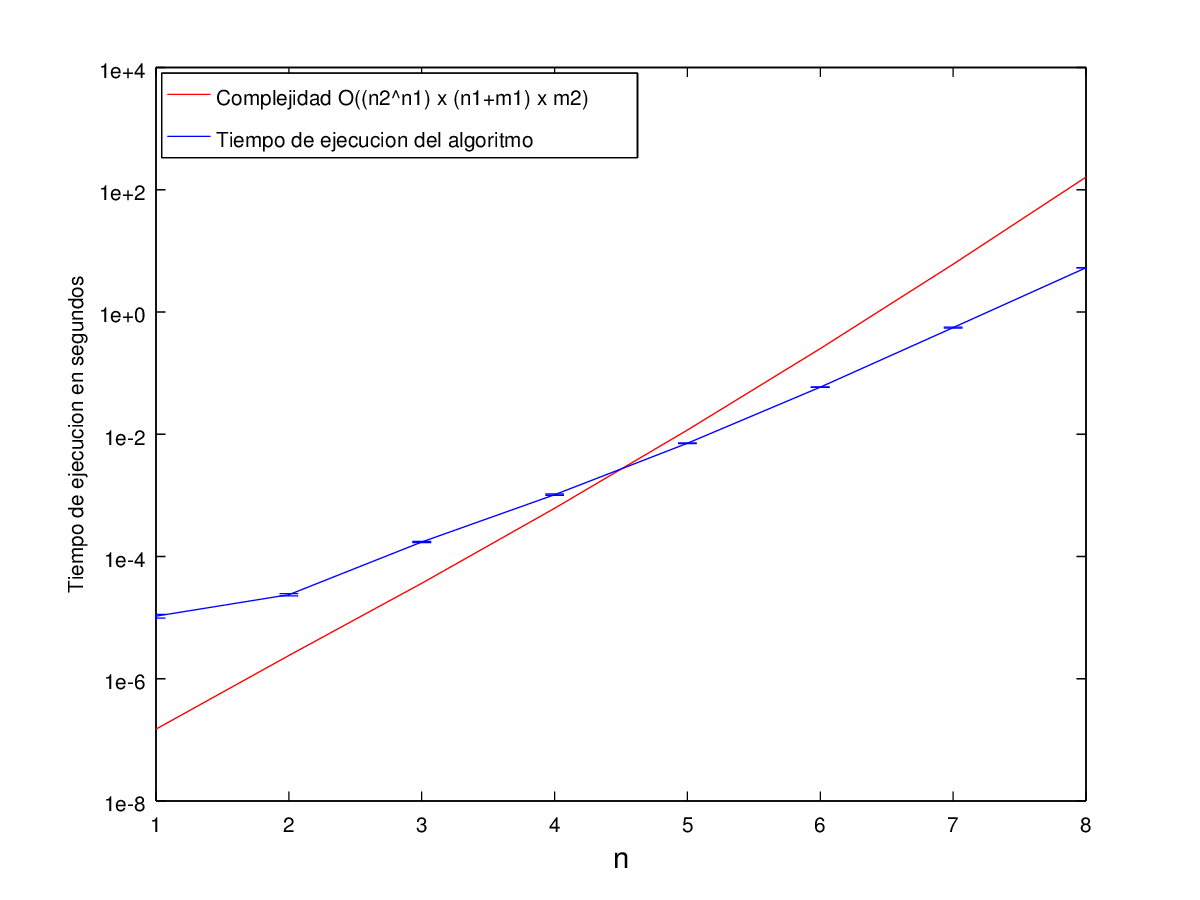
\includegraphics[height=10cm]{graficos/ejercicio2-exp3.png}
       \caption{Experimento 2}
	\end{figure}

\subsubsection*{Observaciones y Conclusiones}\;
En la figura anterior puede observarse como el algoritmo parece respetar la complejidad asintótica propuesta, a pesar de estar para n pequeño por arriba de la curva de complejidad, rápidamente se adecua y se sitúa ligeramente por debajo con similar curvatura).\\
Concluimos entonces que el algoritmo respeta la complejidad asintótica propuesta para el caso de variar manteniendo $n_1=n_2$ y $m_1=m_2$.

\subsubsection*{Experimento 4}\;
\noindent  El objetivo de este experimento fue comparar el tiempo de cómputo requerido por el algoritmo con y sin poda. \\
Para ello, para cada cantidad de nodos se definirá una función para determinar la cantidad de aristas que tendrá el grafo. \\
Se tuvieron en cuenta 2 funciones, con el fin de que el grafo obtenido no sea siempre uno especial y de esta forma poder analizar diferentes casos. Las funciones utilizadas son F3 y F4, ya definidas en el experimento 2, ya que son las dos que no generan grafos especiales, como sí es el caso de F1 y F2.
Para generar los grafos con estas cantidades de aristas y nodos se utilizó el mismo generador que en el experimento 1. 
     	
\subsubsection*{Datos de entrada}\;
\noindent Los valores de $n_1$ tomados fueron desde $1$ hasta $7$. Como es un algoritmo que resuelve un problema de tipo NP-completo no se pudieron utilizar valores grandes ya que el tiempo de ejecución es muy alto. Los valores de $m_1$ están definidos por las funciones F3 y F4.\\
       Los valores de $n_2$ y $m_2$ fueron $10$ y $20$ respectivamente. Estos valores fueron elegidos de forma arbitraria teniendo en cuenta que no se pueden utilizar números muy altos por las razones explicadas anteriormente.\\
        Para generar los grafos de forma aleatoria se utilizó el generador-grafo-rapido.cpp que se encuentra en la carpeta src y para correrlo se utilizó el exp4.sh que se encuentra en la carpeta exp/ejercicio2/exp4. \\
        Con el fin de acercarse a los valores reales y descartar posibles falsos resultados, se ejecuta la resolución del problema para cada una de los valores de $n_1$ cinco veces considerando luego el promedio entre los valores obtenidos pero graficando también el desvío estándar (la cantidad de repeticiones a realizar fue elegida arbitrariamente).\; 
        
\subsubsection*{Resultados}\;

    \begin{figure}[H]
      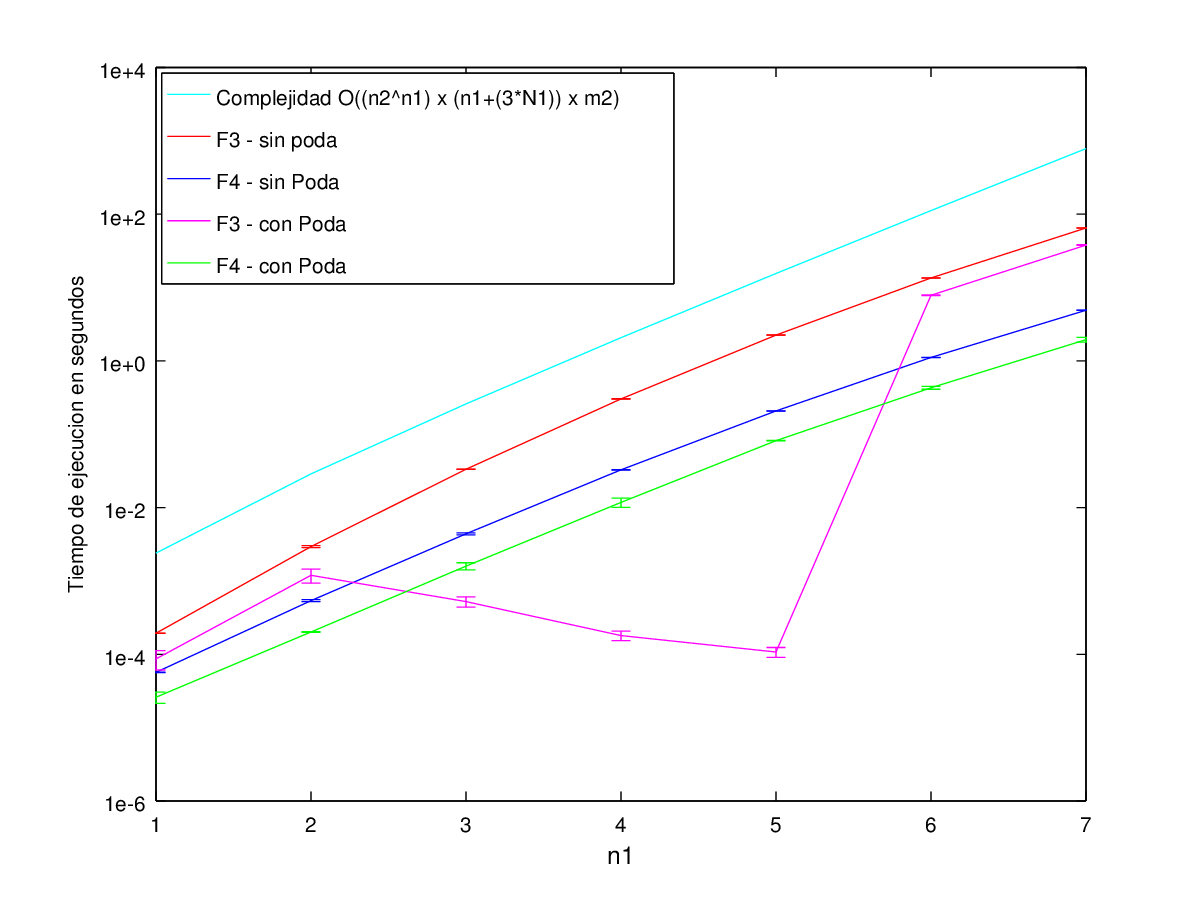
\includegraphics[height=10cm]{graficos/ejercicio2-exp4.png}
       \caption{Experimento 2}
	\end{figure}
\subsubsection*{Conclusiones}\;
En la anterior figura puede observarse como la complejidad pareciera darse igual tanto para el algoritmo con poda como para el sin poda. La efectividad de la poda, en algunos casos, reduce notablemente el tiempo de cómputo.\\
Concluimos entonces de este experimento, que las tanto el algoritmo con poda como sin ella tienen la misma complejidad asintótica, aunque la poda es efectiva en algunos casos para reducir el tiempo de computo.
    
\clearpage
\section{Ejercicio 3}

\subsection{Introducción}
\noindent El problema presentado nos pide encontrar el MCS entre un cografo al que llamaremos $'G'$ (con $\#G$ vértices) y un grafo completo $k_n$ (de $n$ vértices).\\
Para resolver este problema observamos que si el cografo $G$ tiene menor o igual cantidad de vértices que el completo $k_n$ , osea si $\#G \leq n$, el subgrafo común de mayor cantidad de aristas sera  G, pues seguro existe contenido en el completo uno isomorfo a G ya que cada nodo de G lo puedo asignar(en la función isomorfismo $'f'$) a un vértice del completo (porque son menos) y es inmediato ver que en si dos vértices $v_1$,$v_2$ tenían una arista que los unía en G tendrán una una vez aplicado el isomorfismo (habrá arista de $f(v_1)$ a $f(v_2)$) pues es un completo y están todas las aristas posibles.\\
El problema entonces estará en el caso en el que $\#G > n$, es en este caso que observamos que el problema es equivalente a:\\
\emph{'Encontrar el subgrafo $g_n$ de $G$ de $n$ nodos con la mayor cantidad de aristas posibles'}, pues cualquier subgrafo de $G$ de $n$ nodos es isomorfo a un subgrafo de $k_n$, y podemos garantizar que se maximizan las cantidad de aristas como pide el problema ya que si $g_n$ es el grafo de n nodos de mayor cantidad de aristas, no puede haber uno con menos nodos y mas aristas (de haberlo digamos $g_{<n}$ podríamos agregarle $k$ nodos cualesquiera hasta llegar a n, $g_{<n+k}$, y resultaría $cantAristas(g_{<n+k})>cantAristas(g_n)$, contradiciendo la hipótesis de ser $g_n$ el de mayor aristas de $n$ vértices) ni tampoco serviría un subgrafo con mas nodos pues ya dejaría de ser subgrafo de $K_n$.\\
Este último problema entonces es el que intentaremos resolver. Para poder realizarlo en tiempo polinomial aprovecharemos la característica de $G$ de ser cografo.

\subsection{Desarrollo}

\noindent Para resolver este problema entenderemos a los cografos mediante la definición alternativa de cografo, esta es que: los cografos son $K_1$, la unión disjunta de cografos y el 'join' entre 2 cografos (aristas entre todos los nodos de un cografo y todos los nodos del otro).
\subsubsection{Implementación}
La implementación de este algoritmo se divide en 2 grandes etapas:
\begin{enumerate}
\item Creación del cotree:\\
 Un cotree es un árbol enraizado asociado a un cografo. Todo cografo puede representarse univoca mente con un cotree (hay mas de un cotree que representa un mismo cografo pero un cotree determina un único cografo,excepto isomorfismos).\\
 La estructura de cotree es una serie de nodos en forma de árbol en el que cada nodo tiene un id particular. El id de las hojas es un identificador de cada nodo del cografo, mientras que el id de los nodos interiores determina si sus subárboles hijos deben ser unidos disjuntamente o en 'join'.\\
Para armar el cotree el algoritmo será:
\begin{itemize}
\item Si el grafo de entrada es un $k_1$ crear una hoja con el id correspondiente al vértice.
\item Identificar si hay mas de una componente conexa, de haberlas, crear un nodo con el id='Unión' y llamar recursivamente al algoritmo en cada componente conexa y anexar los resultados de cada subproblema como hijos de ese nodo 'Unión'.
\item Si hay una única componente conexa crear un nodo de 'Join' y los hijos serán la llamadas recursivas con el complemento de cada componente conexa del complemento del grafo de entrada.
\end{itemize}
Una vez realizado esto tendremos un cotree válido del cografo.\\
Para simplificar la programación del siguiente inciso procedemos a binarizar el cotree, es decir, expresarlo en un árbol binario. Esto puede hacerse ya que es indistinto para la interpretación del cotree si se unen disjuntamente $x$ cantidad de cografos como una operación atómica o como una sucesión de operaciones binarias; el resultado es el mismo cografo. Lo mismo sucede con el 'join': si quisiéramos hacer un join entre 3 o mas cografos, el resultado sería el mismo al hacer todos los joins juntos que ir tomando de a pares e ir haciendo el join entre esos pares.\\
Para implementar esta binarización recorremos el cotree y para aquellos nodos internos $u$ que tengan mas de 2 hijos, le dejamos uno de esos hijos, $w$, y le ponemos como segundo hijo un nodo del mismo tipo que $u$ (Join o Unión, ya que todos los nodos internos del cotree son, o bien join, o bien unión), llamémoslo $v$. Como hijos de $v$ ponemos a los hijos restantes de $u$ (que son todos los hijos de $u$ menos el nodo $w$). Luego de hacer esa corrección, procedemos a llamar recursivamente a los dos hijos de $u$ ($w$ y $v$).
\item Comparar alternativas:
\begin{itemize}
\item En esta etapa lo que se hará será, dado el cotree $'T'$(binario) asociado al cografo y un entero $n$ (cantidad de vértices del completo), resolveremos el problema de encontrar el subgrafo(del cografo) de $n$ nodos con la mayor cantidad posible de aristas aplicando el siguiente algoritmo(la función 'solución(..)'):\\
tomamos la raíz del cotree $T$ y comparamos todas las posibilidades de tomar n nodos de los sub-cotrees (sus hijos izq y der) para esto llamamos recursivamente a la función iterando(sobre 'i' de 0 a n) la cantidad de vértices a tomar de cada sub-cotree (solución(izq,i) y solución(de,n-i)) y entonces la cantidad de aristas en la solución optima sera una de las siguientes opciones:
  \item la suma de las del izq y der que resultaron ser la combinación máxima, en caso de la raíz ser una 'Unión'.
  \item la suma de las de izq y der que resultaron ser la combinación máxima una vez que a dicha combinación le sumamos el producto de la cantidad de vértices en izq por la cantidad de vértices en der, en caso de ser 'Join'.
 \item 0 aristas tendrá una hoja (un vértice).
 Los nodos pertenecientes a esta solución optima son entonces los cuales se usan en la combinación máxima.
\end{itemize}
Basta entonces llamar a la función solución pasando por parámetro el cotree binario previamente creado y  el tamaño (cantidad de vértices) del completo, para que el algoritmo devuelva los nodos que forman en subgrafo con mayor cantidad de aristas de n nodos.\\
Restaría sólo mostrar el resultado.

\end{enumerate}

\subsubsection{Correctitud}
Para verificar la correctitud de este algoritmo analizaremos 2 incisos.
\begin{enumerate}
\item El subgrafo retornado es un subgrafo(o isomorfo a un subgrafo) tanto del cografo ($G$) como del completo ($K_n$).
\item El subgrafo retornado es optimo (tiene la mayor cantidad de aristas que un subgrafo de ambos puede tener).\\
\\
El inciso 1. es casi inmediato, pues por como se arma el grafo, siempre trabajando sobre subgrafos de $G$, se confirma que el grafo retornado ($'sol'$) es subgrafo de G y como tiene máximo n nodos (tiene exactamente n cuando $\#V(G) > n$ y tiene $\#V(G)$ cuando $n \geq \#V(G)$) tiene que ser subgrafo de $k_n$ pues todo grafo de menos (o igual a n) de n nodos es subgrafo del completo de n nodos ya que si arbitrariamente asignas cada nodo del dicho grafo a cualquiera del completo, todas las aristas del grafo estarán en el completo, por lo tanto concluimos que la solución también es subgrafo de $K_n$.\\ \\
El inciso 2. requiere de un mayor análisis: es óptimo el subgrafo retornado pues las operaciones de Join y de Unión es equivalente hacerlas entre muchas componentes a la vez que hacerlas de a pares como ya explicamos mas arriba en la subsección ``Algoritmo''.\\
Además, dados 2 cografos $C_1$ y $C_2$, subgrafos de $C$ cografo, entrelazados por una Unión o un Join digamos $C:= C_1 \bigtriangleup C_2$ donde $\bigtriangleup$ es operador de Unión o de Join indistintamente.\\
El subgrafo de $C$ de mayor cantidad de aristas de $n_i$ vértices, sera algún $c_1'$ subgrafo de $C_1$ $\bigtriangleup$ algún $c_2'$ subgrafo de $C_2$, pues es evidente que los vértices de éste subgrafo máximo tiene que estar en $C_1$ o en $C_2$ (ya que allí están todos los vértices posibles) y también podemos afirmar que de haber aristas entre $C_1$ y $C_2$ es debido a que $\bigtriangleup$ es un Join (pues si era Unión no habría arista alguna que cruce de $C_1$ a $C_2$) y por lo tanto en ambos casos el subgrafo de $C$ de $n_i$ nodos que maximiza la cantidad de aristas es de la forma:
$c_1' \bigtriangleup c_2'$ con $c_1',c_2'$ subgrafos de sus correspondientes $C_j$  con j=1,2.\\
Como el algoritmo aplica recursivamente este proceso de seleccionar el mejor par $(c_1',c_2')$ (como está descripto mas arriba) probando todos los posibles tamaños de éstos y pidiendo recursivamente los óptimos de subcografos mas chicos. se garantiza que cada paso de selección es optimo y por lo tanto la selección global, con todo el cografo G también lo es. 

\end{enumerate}

\subsection{Complejidad}
La complejidad del algoritmo la vamos a calcular mirando el pseudocódigo del mismo.
Como dijimos anteriormente, el algoritmo se divide en dos grandes etapas:
\begin{itemize}
	\item Creación del cotree
    \item Comparar alternativas
\end{itemize}
\subsubsection*{Creación del cotree}\;
La creación del cotree se divide en dos partes: primero se genera un cotree m-ario, y luego se lo binariza para que el cotree quede binario.
Veamos el pseudocógido de la generación del cotree m-ario: \\
\small{}
\begin{algoritmo}{$make\_cotree$}{$vector<Vertice>* g, Cotree* root$}{}
	\If(\hfill {$\triangleright$ $\mathcal{O}$($N$)}){$obtener\_nodos\_posta($g$) == 1$} {
    	$root->id$ $\gets$ dame\_unico\_nodo($g$) \com*{$\mathcal{O}$($N$)}
        $root->hijos$ $\gets$ $vector<Cotree*>$() \com*{$\mathcal{O}$(1)}
        $root->nodos$.push\_back($root->id$) \com*{$\mathcal{O}$(1)}
        \tipo{return} \com*{$\mathcal{O}$(1)}
    } \Else {
    	$vector<vector<Vertice> >$ componentes $\gets$ separar\_componentes\_conexas($g$) \com*{$\mathcal{O}$($N^2$)}
        \tipo{int} $cc \gets componentes$.size() \com*{$\mathcal{O}$(1)}
        \If(\hfill {$\triangleright$ $\mathcal{O}$(1)}){$cc == 1$} {
        	$root->id \gets$ -1 \com*{$\mathcal{O}$(1)}
            $vector<Vertice> auxx \gets$ complementar(componentes[0]) \com*{$\mathcal{O}$($N^2$)}
            $vector<vector<Vertice> > componentes\_complementadas \gets$ separar\_componentes\_conexas(\&auxx) \com*{$\mathcal{O}$($N^2$)}
            \If(\hfill {$\triangleright$ $\mathcal{O}$(1)}){$componentes\_complementadas.size() != 1$} {
            	\For(\hfill {$\triangleright$ $\mathcal{O}$($N$)}){($i$ = 0; $i < componentes\_complementadas.size()$; $i$++)}{
					Cotree* co\_aux $\gets$ new Cotree() \com*{$\mathcal{O}$(1)}
                    $vector<Vertice> grafo\_aux \gets$ complementar(componentes\_complementadas[$i$]) \com*{$\mathcal{O}$($N^2$)}
                    make\_cotree(\&grafo\_aux, co\_aux) \com*{$\mathcal{O}$(1)}
                    \tipo{iterator} $inicio \gets co\_aux->nodos$.begin() \com*{$\mathcal{O}$(1)}
          			\tipo{iterator} $fin \gets co\_aux->nodos$.end() \com*{$\mathcal{O}$(1)}
                    \While(\hfill {$\triangleright$ $\mathcal{O}$($N$)}){inicio != fin} {
                      $root->nodos.push\_back$(*inicio) \com*{$\mathcal{O}$(1)}
                      inicio++ \com*{$\mathcal{O}$(1)}
                    }
                    $root->hijos.push\_back$(co\_aux) \com*{$\mathcal{O}$(1)}
				}
                \tipo{return} \com*{$\mathcal{O}$(1)}
            }
        } \Else {
        	$root->id \gets$ -2 \com*{$\mathcal{O}$(1)}
            \For(\hfill {$\triangleright$ $\mathcal{O}$($N$)}){$i$ = 0; $i <$ cc; $i$++} {
            	$Cotree* co\_aux \gets$ new Cotree() \com*{$\mathcal{O}$(1)}
                make\_cotree(\&componentes[i], co\_aux) \com*{$\mathcal{O}$(1)}
                \tipo{iterator} $inicio \gets co\_aux->nodos$.begin() \com*{$\mathcal{O}$(1)}
          		\tipo{iterator} $fin \gets co\_aux->nodos$.end() \com*{$\mathcal{O}$(1)}
                \While(\hfill {$\triangleright$ $\mathcal{O}$($N$)}){inicio != fin} {
                  $root->nodos$.push\_back(*inicio) \com*{$\mathcal{O}$(1)}
                  inicio++ \com*{$\mathcal{O}$(1)}
                }
                $root->hijos.push\_back(co\_aux)$ \com*{$\mathcal{O}$(1)}
            }
            \tipo{return} \com*{$\mathcal{O}$(1)}
        }
    }
\end{algoritmo}
\normalsize{}
Esta función usa algunas funciones auxiliares, como $obtener\_nodos\_posta$ que recorre todos los $N$ nodos del cografo, y cuenta la cantidad de nodos que tienen en $true$ el campo $pertenece$, o sea, cuenta la cantidad de nodos que realmente tiene el cografo (si algún nodo tiene el campo $pertenece$ en $false$, ése grafo es un subgrafo del cografo original). Esa función tiene complejidad $\mathcal{O}(N)$ ya que recorre los $N$ nodos y en cada iteración hace pasos constantes (preguntar el valor de $pertenece$ y sumar uno al contador de nodos).\\
Otra función que usa el algoritmo es $dame\_unico\_nodo$ la cual recorre todo el subgrafo del cografo original buscando el único nodo que pertenece a ése subgrafo. También cuenta con complejidad $\mathcal{O}(N)$ ya que recorre todos los nodos del subgrafo y realiza operaciones constantes en cada iteración. \\
Por último, hay otras dos funciones que ejecuta el algoritmo:
\begin{itemize}
	\item $separar\_componentes\_conexas$: separa el grafo en las distintas componentes conexas. Cada componente conexa tiene los $N$ nodos del grafo original, pero sólo sus propios nodos tendrán $true$ en el campo $pertenece$; los demás tendrán $false$.
    \item $complementar$: complementa el grafo pasado por parámetro. Lo hace en $\mathcal{O}(N^2)$ ya que para cada nodo, recorre su lista de adyacencia fijándose qué nodos no están en la lista para agregarlos en la lista de adyacencia correspondiente al mismo nodo en el grafo complemento.
\end{itemize}
En el peor caso (si hubo un Join), en cada iteración se complementa el grafo, que cuesta $\mathcal{O}(N^2)$, y luego se complementa cada componente conexa para llamar recursivamente. En total, entonces tenemos que la complejidad es $\mathcal{O}(N)$*$\mathcal{O}(N^2)$ = $\mathcal{O}(N^3)$, siendo $N$ la cantidad de nodos del cografo. \\ 

Veamos ahora la complejidad de binarizar el cotree: \\
\begin{algoritmo}{$binarizar$}{$Cotree* src$}{}
	\If(\hfill {$\triangleright$ $\mathcal{O}$(1)}){$src->hijos.size() > 2$} {
    	$Cotree* aux \gets$ new Cotree() \com*{$\mathcal{O}$(1)}
    	$aux->id \gets src->id$ \com*{$\mathcal{O}$(1)}
        \For(\hfill {$\triangleright$ $\mathcal{O}$($N'$)}){$i = src->hijos$.size()-1; $i >$ 0; i--} {
        	$aux->hijos$.push\_back($src->hijos$[i]) \com*{$\mathcal{O}$(1)}
            \tipo{iterator} inicio $\gets src->hijos[i]->nodos$.begin() \com*{$\mathcal{O}$(1)}
            \tipo{iterator} fin $\gets src->hijos[i]->nodos$.end() \com*{$\mathcal{O}$(1)}
            \While(\hfill {$\triangleright$ $\mathcal{O}$($N'$)}){inicio != fin} {
              $aux->nodos.push\_back$(*inicio) \com*{$\mathcal{O}$(1)}
              inicio++ \com*{$\mathcal{O}$(1)}
            }
            $src->hijos.pop\_back$() \com*{$\mathcal{O}$(1)}
        }
        $src->hijos$.push\_back(aux) \com*{$\mathcal{O}$(1)}
        binarizar($src->hijos$[0]) \com*{$\mathcal{O}$(1)}
        binarizar($src->hijos$[1]) \com*{$\mathcal{O}$(1)}
    } \Else {
    	\If(\hfill {$\triangleright$ $\mathcal{O}$(1)}){$src->hijos.size() == 2$}{
        	binarizar($src->hijos$[0]) \com*{$\mathcal{O}$(1)}
    		binarizar($src->hijos$[1]) \com*{$\mathcal{O}$(1)}
        } \Else {
        	\If(\hfill {$\triangleright$ $\mathcal{O}$(1)}){$src->hijos.size() == 1$} {
            	binarizar($src->hijos$[0]) \com*{$\mathcal{O}$(1)}
            }
        }
    }
\end{algoritmo}
Sea $N'$ la cantidad de nodos del cotree y $N$ la cantidad de nodos del cografo. Notemos que la función binarizar se va invocando recursivamente por cada nodo del cotree, y si en cada llamada realiza $\mathcal{O}$($N'$) operaciones, en total la función binarizar tiene complejidad $N'$*$\mathcal{O}$($N'$) = $\mathcal{O}$($N'^2$), siendo $N'$ la cantidad de nodos del cotree. Pero como $N' \in \mathcal{O}($N$)$ (ya que si el cotree tiene $N$ hojas, por ser un árbol exactamente binario, tiene $N-1$ nodos internos, entonces la cantidad de nodos del cotree es $N$+$N$-1 = 2$N$-1 = $N'$; notar también que las hojas del cotree corresponden a los nodos del cografo), entonces queda que la complejidad de binarizar es $\mathcal{O}$($N^2$), siendo $N$ la cantidad de nodos del cografo. \\

Por último, tenemos que calcular la complejidad del algoritmo que compara las distintas alternativas: \\
\scriptsize{}
\begin{algoritmo}{$solucion$}{$Cotree* root, int n, vector<AristasNodos>* res$}{}
	\If(\hfill {$\triangleright$ $\mathcal{O}$(1)}){$root->id >= 0$} {
    	AristasNodos aux \com*{$\mathcal{O}$(1)}
        aux.aristas $\gets$ 0 \com*{$\mathcal{O}$(1)}
        $vector<int>$ vec \com*{$\mathcal{O}$(1)}
        vec.push\_back($root->id$) \com*{$\mathcal{O}$(1)}
        aux.nodos $\gets$ vec \com*{$\mathcal{O}$(1)}
        \For(\hfill {$\triangleright$ $\mathcal{O}$($n$)}){$i = 1; i <= n; i++$} {
          (*res)[i] $\gets$ aux \com*{$\mathcal{O}$(1)}
        }
    } \Else {
    	$vector<AristasNodos> vecIzq \gets vector<AristasNodos>(n+1)$ \com*{$\mathcal{O}$($n$)}
        $vector<AristasNodos> vecDer \gets vector<AristasNodos>(n+1)$ \com*{$\mathcal{O}$($n$)}
        solucion($root->hijos$[0], n, \&vecIzq) \com*{$\mathcal{O}$(1)}
        solucion($root->hijos$[1], n, \&vecDer) \com*{$\mathcal{O}$(1)}
        \For(\hfill {$\triangleright$ $\mathcal{O}$($n$)}){$i = 1; i <= n; i++$} {
        	\tipo{int} maxAristas $\gets$ 0 \com*{$\mathcal{O}$(1)}
      		$vector<int>$ noditos \com*{$\mathcal{O}$(1)}
            \For(\hfill {$\triangleright$ $\mathcal{O}$($n$)}){$j = 0; j <= i; j++$} {
            	\tipo{int} aristasI $\gets$ 0 \com*{$\mathcal{O}$(1)}
                \tipo{int} aristasD $\gets$ 0 \com*{$\mathcal{O}$(1)}
                \tipo{int} aristasTotales \com*{$\mathcal{O}$(1)}
                $vector<int>$ vec \com*{$\mathcal{O}$(1)}
                \If(\hfill {$\triangleright$ $\mathcal{O}$(1)}){j != 0} {
                	aristasI $\gets$ vecIzq[j].aristas \com*{$\mathcal{O}$(1)}
                    \tipo{iterator} inicio $\gets$ vecIzq[j].nodos.begin() \com*{$\mathcal{O}$(1)}
                    \tipo{iterator} fin $\gets$ vecIzq[j].nodos.end() \com*{$\mathcal{O}$(1)}
                    \While{inicio != fin} {
                      vec.push\_back(*inicio) \com*{$\mathcal{O}$(1)}
                      inicio++ \com*{$\mathcal{O}$(1)}
                    }
                }
                \If(\hfill {$\triangleright$ $\mathcal{O}$(1)}){i-j != 0} {
                	aristasD $\gets$ vecDer[i-j].aristas \com*{$\mathcal{O}$(1)}
                    \tipo{iterator} inicio $\gets$ vecDer[i-j].nodos.begin() \com*{$\mathcal{O}$(1)}
                    \tipo{iterator} fin $\gets$ vecDer[i-j].nodos.end() \com*{$\mathcal{O}$(1)}
                    \While{inicio != fin} {
                      vec.push\_back(*inicio) \com*{$\mathcal{O}$(1)}
                      inicio++ \com*{$\mathcal{O}$(1)}
                    }
                }
                aristasTotales $\gets$ aristasI + aristasD \com*{$\mathcal{O}$(1)}
                \If(\hfill {$\triangleright$ $\mathcal{O}$(1)}){$root->id == -1$} {
                	aristasTotales $\gets$ aristasTotales + (vecIzq[j].nodos.size()*vecDer[i-j].nodos.size()) \com*{$\mathcal{O}$(1)}
                }
                \If(\hfill {$\triangleright$ $\mathcal{O}$(1)}){$aristasTotales >= maxAristas \&\& vec.size() >= noditos.size()$} {
                	maxAristas $\gets$ aristasTotales \com*{$\mathcal{O}$(1)}
          			noditos $\gets$ vec \com*{$\mathcal{O}$(1)}
                }
            }
            AristasNodos aux \com*{$\mathcal{O}$(1)}
            aux.aristas $\gets$ maxAristas \com*{$\mathcal{O}$(1)}
            aux.nodos $\gets$ noditos \com*{$\mathcal{O}$(1)}
            (*res)[i] $\gets$ aux \com*{$\mathcal{O}$(1)}
        }
    }
\end{algoritmo}
\normalsize{}
Sea $n$ la cantidad de nodos del grafo completo. Esta función se va invocando recursivamente para cada nodo del cotree. Si $N'$ es la cantidad de nodos del cotree, entonces la complejidad del algoritmo tiene un factor multiplicativo de $\mathcal{O}(N')$. Por otro lado, el algoritmo recorre un vector de tamaño $n$, rellenando cada posición del mismo. Para rellenar cada $i$ posición, tiene que iterar $j=0$ hasta $i$ eligiendo $j$ nodos del subárbol izquierdo y $i-j$ nodos del subárbol derecho. Al mismo tiempo, se agregan los $i-j+j$=$i$ nodos al vector $vec$. Como $i$ va hasta $n$, el total de complejidad de todo ese recorrido es $\mathcal{O}(n)$*$\mathcal{O}(n)$*$\mathcal{O}(n)$ = $\mathcal{O}(n^3)$. No olvidándonos del factor multiplicativo $\mathcal{O}(N')$, la complejidad total del algoritmo ``solución'' es $\mathcal{O}(N')$*$\mathcal{O}(n^3)$ = $\mathcal{O}(N'*n^3)$, donde $N'$ es la cantidad de nodos del cotree y $n$ es la cantidad de nodos del grafo completo. Recordemos por el análisis del algoritmo anterior que $N'$ pertenece a la misma clase de complejidad que $N$ (que es la cantidad de nodos del cografo), entonces la complejidad final del algoritmo es $\mathcal{O}(N*n^3)$ \\

Finalmente, la complejidad total del algoritmo de este ejercicio es la suma de las complejidades anteriormente calculadas. Usando álgebra de órdenes, tenemos:
\begin{itemize}
	\item Armar cotree: $\mathcal{O}(N^3)$, $N$ = cantidad de nodos del cografo.
    \item Binarizar cotree: $\mathcal{O}(N^2)$, $N$ = cantidad de nodos del cografo.
    \item Comparar Alternativas: $\mathcal{O}(N*n^3)$, $N$ = cantidad de nodos del cografo y $n$ = cantidad de nodos del grafo completo.
\end{itemize}
Entonces la complejidad de este ejercicio es de $\mathcal{O}(N^3)$ + $\mathcal{O}(N^2)$ + $\mathcal{O}(N*n^3)$ = $\mathcal{O}(N^3)$ + $\mathcal{O}(N*n^3)$ = $\mathcal{O}(N*(N^2+n^3))$
Como la complejidad obtenida es polinomial, el problema de MCS con estas propiedades (de tener un cografo y un grafo completo) es un problema \textit{bien resuelto}

\subsection{Experimentación}
\noindent El algoritmo toma un cografo de $n$ nodos y un grafo completo $K_n$. La cantidad de aristas del cografo está sujeta a la cantidad de nodos y a cómo estos nodos están relacionados (por Joins o por Uniones). Para la experimentación, entonces, será necesario variar la cantidad de nodos tanto del cografo como del completo. Las operaciones que relacionan a los nodos (Unión o Join) serán tomadas al azar y éstas inducirán la cantidad de aristas del cografo.\\


		\subsubsection*{Experimento 1}\; 
        \noindent  El objetivo de este experimento será extraer conclusiones acerca de la variación en el tiempo de cómputo requerido por el algoritmo para distintos valores de $n$ del cografo, con el fin de determinar su complejidad. \\
   Se utilizará un generador de cografos y grafos completos que recibe la cantidad de nodos de cada uno, $n_1$ cografo y $n_2$ completo, y genera un cografo de $n_1$ nodos y un completo de $n_2$ nodos.

     	\subsubsection*{Datos de entrada}\;
\noindent Los valores de $n_1$ tomados fueron desde $10$ hasta $200$ de $20$ en $20$.\\
       Los valores de $n_2$ y $m_2$ fueron $200$ y $19900$ respectivamente. El valor de $n$ fue elegido de forma arbitraria y al ser un completo $m_2$ deberá tomar ese valor.\\
        Para generar los grafos de forma aleatoria se utilizó el generador-grafosEspeciales.cpp que se encuentra en la carpeta src y para correrlo se utilizó el exp1.sh que se encuentra en la carpeta exp/ejercicio3/exp1. \\
        Con el fin de acercarse a los valores reales y descartar posibles falsos resultados, se ejecuta la resolución del problema para cada una de los valores de $n_1$ cinco veces considerando luego el promedio entre los valores obtenidos pero graficando también el desvío estándar (la cantidad de repeticiones a realizar fue elegida arbitrariamente).\; 

\subsubsection*{Resultados}\;
        
            \begin{figure}[H]
      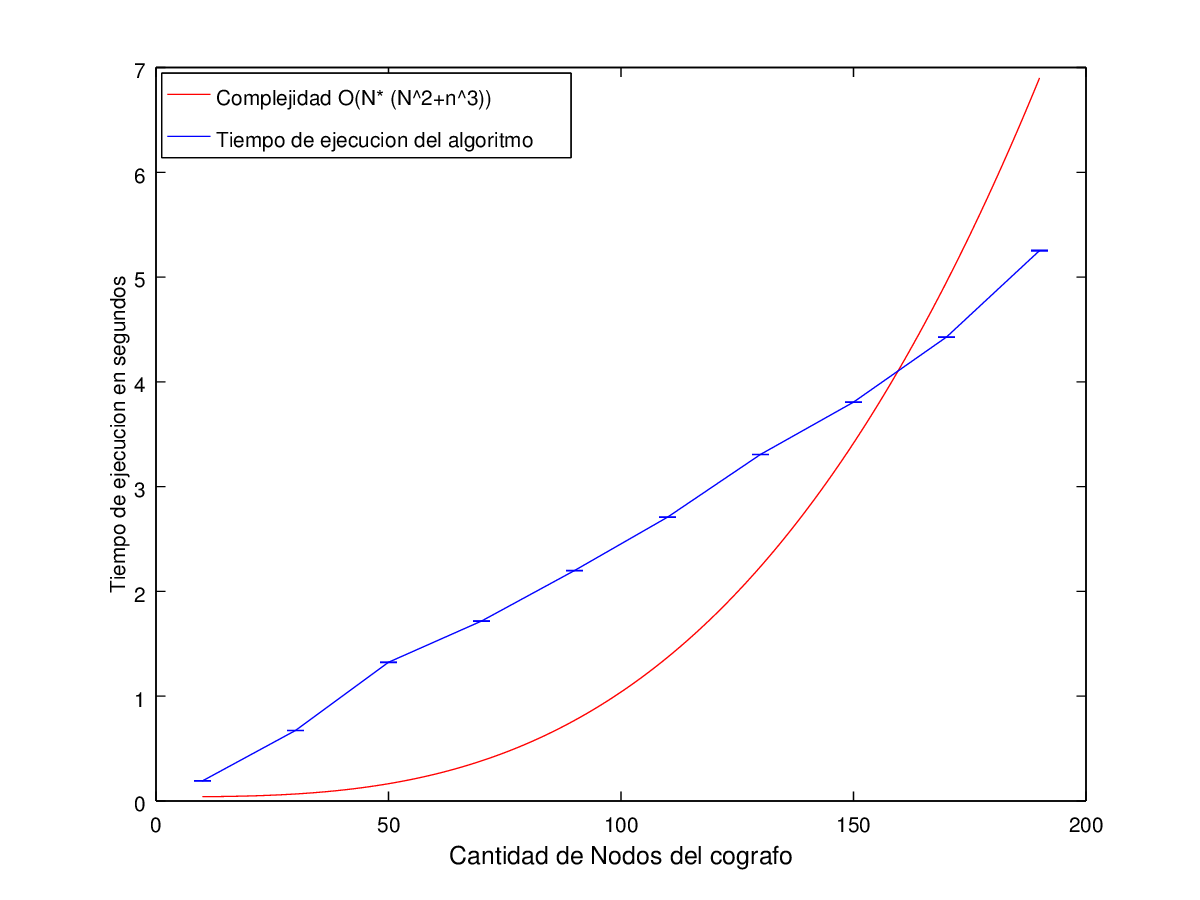
\includegraphics[height=10cm]{graficos/ejercicio3-exp1.png}
       \caption{Experimento 1}
	\end{figure}
        
     	\subsubsection*{Conclusiones}\;
\noindent Se puede observar del gráfico que se respeta la complejidad asintótica propuesta para el algoritmo en caso de hacer variar el $n$ dejando estático el $n$. A pesar de que la curva de tiempo de cómputo esté por encima de la complejidad, a partir de cierto punto, se coloca por debajo de ésta con una curvatura similar o menos pronunciada.
        

\subsubsection*{Experimento 2}\; 

        \noindent Este experimento es similar al anterior pero ahora se variará la cantidad de nodos de cografo ($n_1$) y a la vez también el tamaño (cantidad de nodos) del completo ($n_2$). Lo que trataremos de recrear y observar cual será el comportamiento del tiempo de cómputo a medida que el cografo crece en cantidad de nodos para algún completo arbitrario.

     	\subsubsection*{Datos de entrada}\;
\noindent Los valores de $n_1$ tomados fueron desde $10$ hasta $200$ de $20$ en $20$.\\
       Los valores de $n_2$ son $n_1$/2 para cada $n_1$. \\
        Para generar los grafos de forma aleatoria se utilizó el generador-grafosEspeciales.cpp que se encuentra en la carpeta src y para correrlo se utilizó el exp2.sh que se encuentra en la carpeta exp/ejercicio3/exp2. \\
        Con el fin de acercarse a los valores reales y descartar posibles falsos resultados, se ejecuta la resolución del problema para cada una de los valores de $n_1$ cinco veces considerando luego el promedio entre los valores obtenidos pero graficando también el desvío estándar (la cantidad de repeticiones a realizar fue elegida arbitrariamente).\; 

\subsubsection*{Resultados}\;

            \begin{figure}[H]
      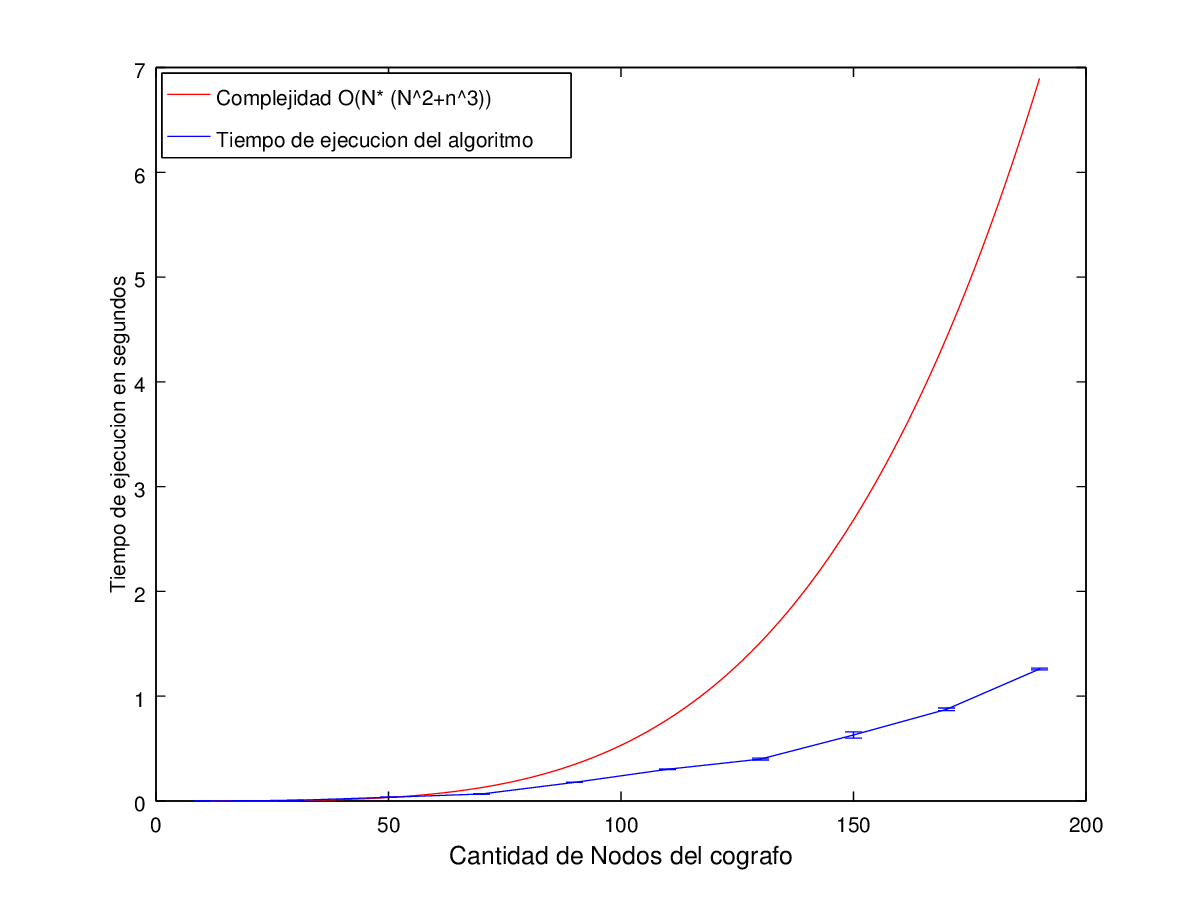
\includegraphics[height=10cm]{graficos/ejercicio3-exp2.png}
       \caption{Experimento 2}
	\end{figure}
        
     	\subsubsection*{Conclusiones}\;
        Se observa que también se respeta la complejidad predicha ya que se ve que la curva del tiempo de ejecución se sitúa por debajo de la curva de complejidad asintótica.\\
        Podemos concluir entonces del experimento que el algoritmo respeta la complejidad propuesta.\\
Pareciera  que la curva de complejidad calculada es de un orden superior al la curva del tiempo de ejecución, esto podría significar, que podría hilarse mas fino en la complejidad propuesta o que quizás el grafo generado al azar y el completo no entrarían dentro del peor caso.










\clearpage
\section{Ejercicio 4}

\subsection{Introducción}
\noindent El objetivo de este ejercicio es resolver nuevamente el problema de MCS, pero esta vez con una heurística constructiva golosa, ya que suponemos que resolver el problema de forma exacta no se puede hacer en tiempo polinomial, pero sí podemos implementar un algoritmo heurístico que se ejecute eficientemente (tiempo polinomial) aunque no garantice la solución óptima.\\
La heurística constructiva golosa es un algoritmo que va armando la solución tomando en cada paso la mejor elección a nivel local de un conjunto de elecciones posibles, es decir, para cada paso, tomar la decisión que sea la más conveniente en ese momento.\\
Esto puede generar que la solución no sea la óptima real ya que ésta última podría requerir mirar soluciones que no sean las óptimas en el momento pero que luego llevarán a la mejor solución posible. 

\subsection{Heurística}
\noindent El algoritmo recibe dos grafos y se quiere hallar al máximo subgrafo común entre ellos. Sea $G1$ el que tiene la menor cantidad de nodos y $G2$ el otro. Si ambos tienen igual cantidad de nodos es indistinto cual es $G1$ y cual es $G2$.\\
Sea el vector mapeo, igual al desarrollado en el ejercicio 2. Dado un mapeo, se busca cuál es el conjunto de aristas que tienen en común ambos grafos renombrando cada nodo $i$ de $G1$ como $mapeo[i]$, es decir, el nodo que antes era el nodo $i$ ahora se llamará $mapeo[i]$.\\
Para este ejercicio la heurística que se utilizará es la que mapea los nodos de forma ordenada por grados. Sea nodosPorGrados un vector que ordena los nodos de un grafo según sus grados de mayor a menor. Lo que queremos hallar es el mapeo que cumple que el nodo $i$ $\in$ $G1$ está mapeado con el nodo $j$ $\in$ $G2$ sí y sólo sí el nodo $i$ y el nodo $j$ ocupan la misma posición en el vector nodosPorGrados para cada uno de los grafos.\\

\noindent Esta heurística es válida ya que mapear ordenadamente por grados hace que, en muchos casos, la cantidad de aristas que puede ser tomada en cuenta sea la máxima posible. Si se mapea el que tiene menor grado con el de mayor grado del otro grafo lo que puede pasar es que, por ejemplo, quede uno de grado cero con uno de grado muy alto, entonces todas las aristas incidentes la de mayor grado no pueden ser tenidas en cuenta para el calculo del máximo común subgrafo. Lo que puede pasar es que por más que se mapee de esta manera, las conexiones entre los nodos queden totalmente diferentes entre los grafos. Por ejemplo, sea $G1$ el grafo $Cn$ y $G2$ un grafo compuesto por $k$ componentes conexas en donde cada una de ellas es un grafo estrella con un nodo de grado mayor o igual a 2. Supongamos que la cantidad de nodos de $Cn$ es menor que $k$. $Cn$ tiene todos nodos de grado 2, entonces a cada nodo de $Cn$ se lo mapeará con un nodo del centro de las estrellas generando así que no haya ninguna arista en común para este mapeo.\\
%supongamos que el grafo que se tiene es un conjunto de grafos estrella y el otro grafo es un ciclo (Cn). Luego el Cn tiene todos nodos de grado 2 pero el conjunto de estrella tiene tantos nodos como subgrafos estrellas haya con grados mayores o iguales a dos. Entonces si la cantidad de nodos de Cn es menor que la cantidad de componentes conexas del otro, a cada nodo de Cn se lo mapeará con un nodo del centro de las estrellas generando así que no haya ninguna arista en común para este mapeo.
\begin{figure}[H]

\hspace*{\fill} 
\begin{tikzpicture}[scale= 0.6]
\node[draw,circle,thick,fill,red](0) at (1,0){}; \\
 \node[draw,circle,thick,fill,orange](1) at (3,2.5){}; \\
 \node[draw,circle,thick,fill,yellow](2) at (6,2.5){}; \\
 \node[draw,circle,thick,fill,green](3) at (8,0){}; \\
 \node[draw,circle,thick,fill,blue](4) at (6,-2.5){}; \\
 \node[draw,circle,thick,fill,purple](5) at (3,-2.5){}; \\

% \draw [thick,->] (a) to [out=120,in=180] (b);
 \draw [thick] (0) -- (1);
 \draw [thick] (1) -- (2);
 \draw [thick] (2) -- (3);
 \draw [thick] (3) -- (4);
 \draw [thick] (4) -- (5);
 \draw [thick] (0) -- (5);
\end{tikzpicture}
\hspace{\fill} 
\caption{$G1=C_{6}$}
\end{figure}

\begin{figure}[H]

%\hspace*{\fill} 
\begin{tikzpicture}[scale= 0.5]
 \node[draw,circle,thick,fill,red](0) at (0,0){}; \\
 \node[draw,circle](1) at (2,0){}; \\
 \node[draw,circle](2) at (0,2){}; \\
 \node[draw,circle](3) at (-2,0){}; \\
 \node[draw,circle](4) at (0,-2){}; \\

 \node[draw,circle,thick,fill,orange](5) at (6,0){}; \\
 \node[draw,circle](6) at (8,0){}; \\
 \node[draw,circle](7) at (6,2){}; \\
 \node[draw,circle](8) at (6,-2){}; \\
 \node[draw,circle](9) at (4,0){}; \\
 
 \node[draw,circle,thick,fill,yellow](10) at (12,0){}; \\
 \node[draw,circle](11) at (14,0){}; \\
 \node[draw,circle](12) at (12,2){}; \\
 \node[draw,circle](13) at (12,-2){}; \\
 \node[draw,circle](14) at (10,0){}; \\
 
 \node[draw,circle,thick,fill,green](15) at (18,0){}; \\
 \node[draw,circle](16) at (20,0){}; \\
 \node[draw,circle](17) at (18,2){}; \\
 \node[draw,circle](18) at (18,-2){}; \\
 \node[draw,circle](19) at (16,0){}; \\
 
 \node[draw,circle,thick,fill,blue](20) at (24,0){}; \\
 \node[draw,circle](21) at (26,0){}; \\
 \node[draw,circle](22) at (24,2){}; \\
 \node[draw,circle](23) at (24,-2){}; \\
 \node[draw,circle](24) at (22,0){}; \\
 
 \node[draw,circle,thick,fill,purple](25) at (30,0){}; \\
 \node[draw,circle](26) at (32,0){}; \\
 \node[draw,circle](27) at (30,2){}; \\
 \node[draw,circle](28) at (30,-2){}; \\
 \node[draw,circle](29) at (28,0){}; \\

% \draw [thick,->] (a) to [out=120,in=180] (b);
 \draw [thick] (0) -- (1);
 \draw [thick] (0) -- (2);
 \draw [thick] (0) -- (3);
 \draw [thick] (0) -- (4);
 
 \draw [thick] (5) -- (6);
 \draw [thick] (5) -- (7);
 \draw [thick] (5) -- (8);
 \draw [thick] (5) -- (9);
 
 \draw [thick] (10) -- (11);
 \draw [thick] (10) -- (12);
 \draw [thick] (10) -- (13);
 \draw [thick] (10) -- (14);

 \draw [thick] (15) -- (16);
 \draw [thick] (15) -- (17);
 \draw [thick] (15) -- (18);
 \draw [thick] (15) -- (19);
 
 \draw [thick] (20) -- (21);
 \draw [thick] (20) -- (22);
 \draw [thick] (20) -- (23);
 \draw [thick] (20) -- (24);
 
 \draw [thick] (25) -- (26);
 \draw [thick] (25) -- (27);
 \draw [thick] (25) -- (28);
 \draw [thick] (25) -- (29);


\end{tikzpicture}
%\hspace{\fill} 
\caption{$G2$}
\end{figure}

\noindent En las figuras se muestra en colores el mapeo que se genera con la heurística golosa. Por ejemplo, el nodo rojo en $G1$ se mapea con el nodo rojo en $G2$. Este mapeo genera la siguiente respuesta: 

\begin{figure}[H]

\hspace*{\fill} 
\begin{tikzpicture}[scale= 0.6]
\node[draw,circle,thick](0) at (0,0){}; \\
 \node[draw,circle,thick](1) at (3,0){}; \\
 \node[draw,circle,thick](2) at (6,0){}; \\
 \node[draw,circle,thick](3) at (9,0){}; \\
 \node[draw,circle,thick](4) at (12,0){}; \\
 \node[draw,circle,thick](5) at (15,0){}; \\
\end{tikzpicture}
\hspace{\fill} 
\caption{Grafo solución según heurística golosa}
\end{figure}

\noindent Pero la solución real es la siguiente: 
\begin{figure}[H]

\hspace*{\fill} 
\begin{tikzpicture}[scale= 0.6]
\node[draw,circle,thick](0) at (0,0){}; \\
 \node[draw,circle,thick](1) at (0,2){}; \\
 \node[draw,circle,thick](2) at (2,0){}; \\
 \node[draw,circle,thick](3) at (6,0){}; \\
 \node[draw,circle,thick](4) at (6,2){}; \\
 \node[draw,circle,thick](5) at (8,0){}; \\

% \draw [thick,->] (a) to [out=120,in=180] (b);
 \draw [thick] (0) -- (1);
 \draw [thick] (0) -- (2);
 \draw [thick] (3) -- (4);
 \draw [thick] (3) -- (5);
\end{tikzpicture}
\hspace{\fill} 
\caption{Grafo solución}
\end{figure}


\subsection{Implementación}

El algoritmo se comporta de la siguiente manera:
\begin{itemize}
\item Primero se ordenan los nodos de ambos grafos por grado, de mayor a menor generando así un vector que en cada posición contiene una tupla compuesta por el numero de nodo y su grado. \\
\begin{figure}[H]
\centering
      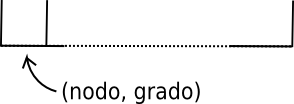
\includegraphics[height=1.5cm]{graficos/ejercicio4-1.png}
      \caption{vector gradosGrafo}
\end{figure}
\item Sabemos que el grafo solución va a tener la misma cantidad de nodos que G1 ya que el grafo formado por los nodos del grafo de menor tamaño sin aristas es un subgrafo de G2. Por lo tanto, lo que buscamos es agregarle la mayor cantidad de aristas que tengan en común los dos grafos iniciales.
\item Luego se tienen dos vectores, uno por cada grafo, donde se encuentran los nodos ordenados por grados. Ahora se mapea el nodo que se encuentra en la posición $i$ del vector correspondiente al grafo G1 con el nodo de la posición $i$ del grafo G2. Esto se hace para $i$ entre 0 y el tamaño del vector correspondiente a G1, es decir, entre 0 y la cantidad de nodos de G1. \\
\begin{figure}[H]
\centering
      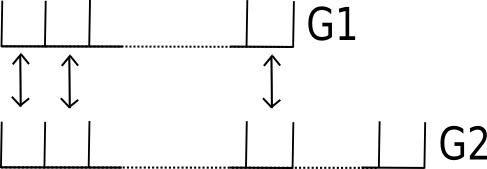
\includegraphics[height=2cm]{graficos/ejercicio4-2.png}
      \caption{Mapeo de grafos}
\end{figure}
\item Con este mapeo obtenido se calculan las aristas que tienen en común ambos grafos obteniendo así la solución al problema. 

\end{itemize}

\begin{algoritmo}{MCSgoloso}{\In{GrafoGrande}{vector(vector(int))}, \In{GrafoChico}{vector(vector(int))}, \In{gradosGrafoGrande}{vector(pair(int, int))}, \In{gradosGrafoGrande}{vector(pair(int, int))}}{vector(pair(int, int))}

	\For{(i = 0...gradosGrafoChico.size() - 1)}{
		mapeo[gradosGrafoChico[i].first] = gradosGrafoGrande[i].first; 
	}
	
	\tipo{vector(pair(int, int))} respuesta;
	respuesta = calcularConjAristas(mapeo, grafoChico, grafoGrande);
	return respuesta;      

\end{algoritmo}

\subsubsection*{Correctitud}
\noindent Veamos ahora que el resultado final es un subgrafo. Dado un mapeo válido se busca cuál es el conjunto de aristas que tienen en común ambos grafos renombrando cada nodo $i$ de G1 como $mapeo[i]$, es decir, el nodo que antes era el nodo $i$ ahora se llamará $mapeo[i]$.\\
Esto construye un subgrafo de ambos ya que para generar la respuesta se buscan las aristas que pertenecen a ambos grafos. 


\subsection{Complejidad}
Por claridad supondremos que el grafo G1 es el de menor cantidad de vértices (si son iguales, es indistinto).\\
El algoritmo implementado consta de 2 grandes etapas (aparte de las de recibir los datos y la de mostrarlos): la de ordenar por grados a los vértices, y la de mapear en orden y ver cuales son las aristas correspondientes que pueden ponerse en el mapeo.\\
Para la etapa de ordenar por grados, lo único que se hace es recorrer los grafos e ir guardando en un vector (uno por grafo) cada nodo con su grado (se tarda $\mathcal{O}(n_1+m_1)$ en recorrer el primero grafo y se tarda $\mathcal{O}(n_2+m_2)$ en recorrer el segundo). Luego se procede a ordenar por grado usando la función $sort(..)$ que, como esta especificado en la documentación de $C++$ (http://www.cplusplus.com/reference/algorithm/sort/), es $\mathcal{O}(n*log(n))$, con $n$ el tamaño el vector a ordenar. En particular, en este caso se tarda $\mathcal{O}(n_1*log(n_1)+n_2*log(n_2))$ en ordenar ambos vectores, que es igual a $\mathcal{O}(n_2*log(n_2))$ dado que asumimos a G2 el mas grande en cantidad de nodos.\\
En la segunda etapa, lo que se hace es mapear en el orden que quedaron luego de aplicar el sort y recorrer el grafo más chico (para este caso el G1) preguntando si por cada una de sus aristas, existe su equivalente en G2 luego de aplicar el mapeo. Recorrer las aristas de este G1 tiene complejidad $\mathcal{O}(n_1+m_1)$; para cada arista de este, se consulta en en su mapeo (la transformación del mapeo se realiza en $\mathcal{O}(1)$ pues es leer una posición determinada de un vector) los vecinos de el vértice de G2 correspondiente, esto (como sólo se recorren los vecinos de un único nodo ya determinado de G2) tarda $\mathcal{O}(m_2)$, por lo que en total la complejidad de esta etapa es $\mathcal{O}((n_1+m_1)*m_2)$.\\
Concluimos entonces que entre ambas etapas el orden de complejidad será la suma $\mathcal{O}((n_1+m_1)*m_2+n_2*log(n_2))$.


\subsection{Experimentación}
\noindent El algoritmo toma dos grafos para calcular el máximo subgrafo común, entonces para tomar las mediciones y determinar el tiempo de cómputo de la heurística, generalmente, se modificarán únicamente las cantidades de nodos y aristas de uno de ellos. \\
Sea $n_1$ y $m_1$ la cantidad de nodos y aristas del grafo que se modificará para tomar las mediciones respectivamente y $n_2$, $m_2$ la cantidad de nodos y aristas del grafo al que se le dejarán constantes las cantidades de nodos y aristas, aunque en cada caso podrán utilizarse grafos distintos por con la misma cantidad de vértices y de aristas.
    
	\subsubsection*{Experimento 1}\; 
\noindent  El objetivo de este experimento fue extraer conclusiones acerca de la variación en el tiempo de cómputo requerido por el algoritmo para distintos valores de $m_1$, con el fin de determinar su complejidad, dejando $n_1$ fijo. \\
   Para ello se utilizará un generador de grafos que funciona de la siguiente manera: dada una cantidad de vértices y aristas, en cada paso crea una nueva arista con extremos válidos (es decir, entre 0 y la cantidad de vértices - 1) y que no este repetida (que no haya sido creada todavía). 
   
     	\subsubsection*{Datos de entrada}\;
        \noindent Para correr el algoritmo con poda los valores de $m_1$ tomados fueron desde $0$ hasta $19900$ de $100$ en $100$. El valor de $n_1$ fue $200$.\\
       Los valores de $n_2$ y $m_2$ fueron $200$ y $2500$ respectivamente. Estos valores fueron elegidos de forma arbitraria.\\
        Para generar los grafos de forma aleatoria se utilizó el generador-grafo-rapido.cpp que se encuentra en la carpeta src y para correrlo se utilizó el exp1.sh que se encuentra en la carpeta exp/ejercicio4/exp1. \\
        Con el fin de acercarse a los valores reales y descartar posibles falsos resultados, se ejecuta la resolución del problema para cada una de los valores de $m_1$ siete veces considerando luego el promedio entre los valores obtenidos pero graficando también el desvío estándar (la cantidad de repeticiones a realizar fue elegida arbitrariamente).\; 
        \subsubsection*{Resultados}\;

    \begin{figure}[H]
      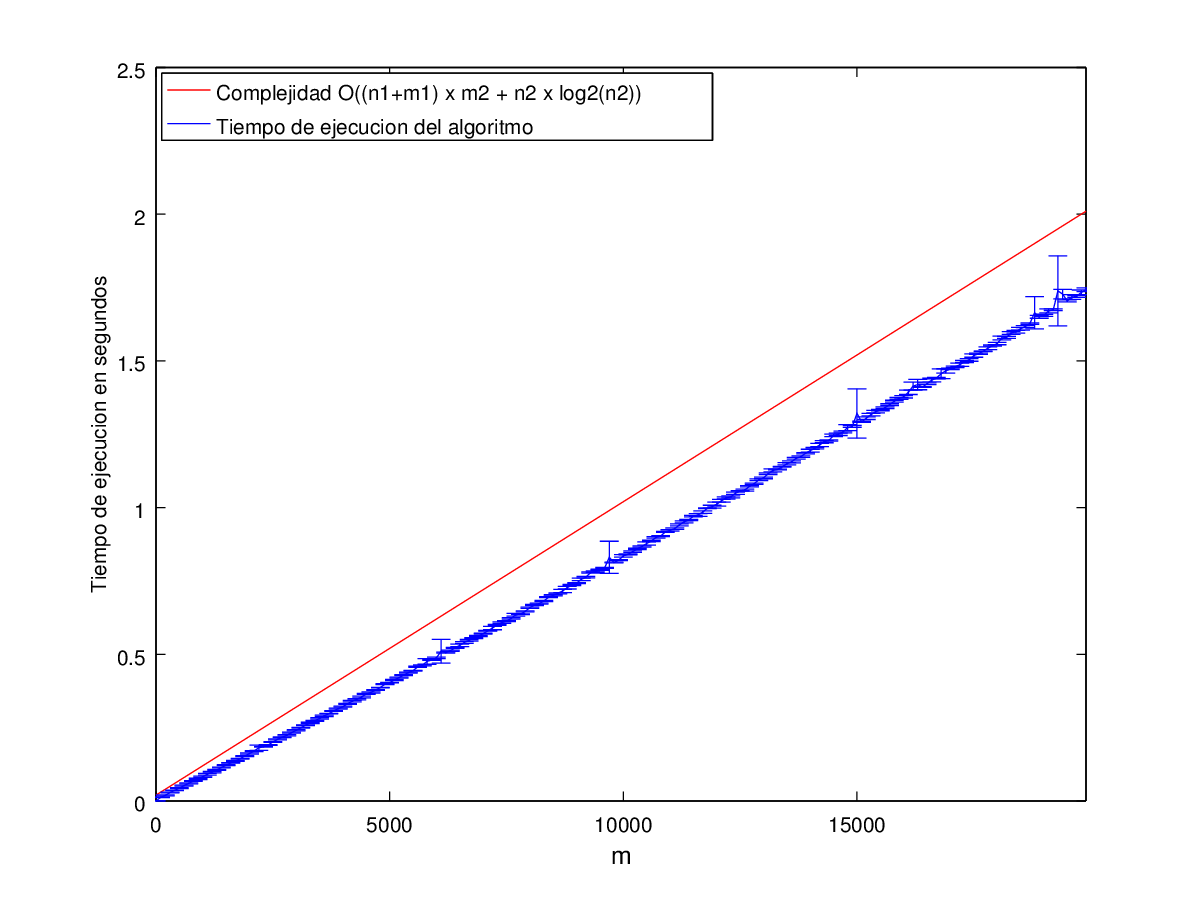
\includegraphics[height=10cm]{graficos/ejercicio4-exp1.png}
       \caption{Experimento 1}
	\end{figure}
        
\subsubsection*{Conclusiones}\;
Se concluye de observar el gráfico que se cumple la complejidad esperada para este caso en el que se mantiene la cantidad de nodos y se varía la cantidad de aristas, pues los tiempos de ejecución se mantienen por debajo de la línea de complejidad predicha.
    
    \subsubsection*{Experimento 2}\; 
    \noindent Este experimento es similar al anterior, pero ahora se varía la cantidad de nodos. Para ello, para cada cantidad de nodos se definirá una función para determinar la cantidad de aristas que tendrá el grafo. \\
    Se tuvieron en cuenta 4 funciones, con el fin de que el grafo obtenido no sea siempre uno especial y de esta forma poder analizar diferentes casos. 
        \begin{itemize}
        \item F1($n_1$) = $n_1$($n_1$-1))/2 = $m_1$ 
        \item F2($n_1$) = $n_1$-1 = $m_1$ 
        \item F3($n_1$) = 3$n_1$ = $m_1$
        \item F4($n_1$) = $n_1^{2}$/10 = $m_1$
		\end{itemize} 
 Para generar los grafos con estas cantidades de aristas y nodos se utilizó el mismo generador que en el experimento anterior.       
        
        
        \subsubsection*{Datos de entrada}\;
        
        \noindent Los valores de $n_1$ tomados fueron desde $100$ hasta $320$ de $20$ en $20$. \\
       Los valores de $n_2$ y $m_2$ fueron $320$ y $2500$ respectivamente. Estos valores fueron elegidos de forma arbitraria.\\
        Para generar los grafos de forma aleatoria se utilizó el generador-grafo-rapido.cpp que se encuentra en la carpeta src y para correrlo se utilizó el exp2.sh que se encuentra en la carpeta exp/ejercicio4/exp2. \\
        Con el fin de acercarse a los valores reales y descartar posibles falsos resultados, se ejecuta la resolución del problema para cada una de los valores de $n_1$ cinco veces considerando luego el promedio entre los valores obtenidos pero graficando también el desvío estándar (la cantidad de repeticiones a realizar fue elegida arbitrariamente).\; 
        
         \subsubsection*{Resultados}\;

    \begin{figure}[H]
      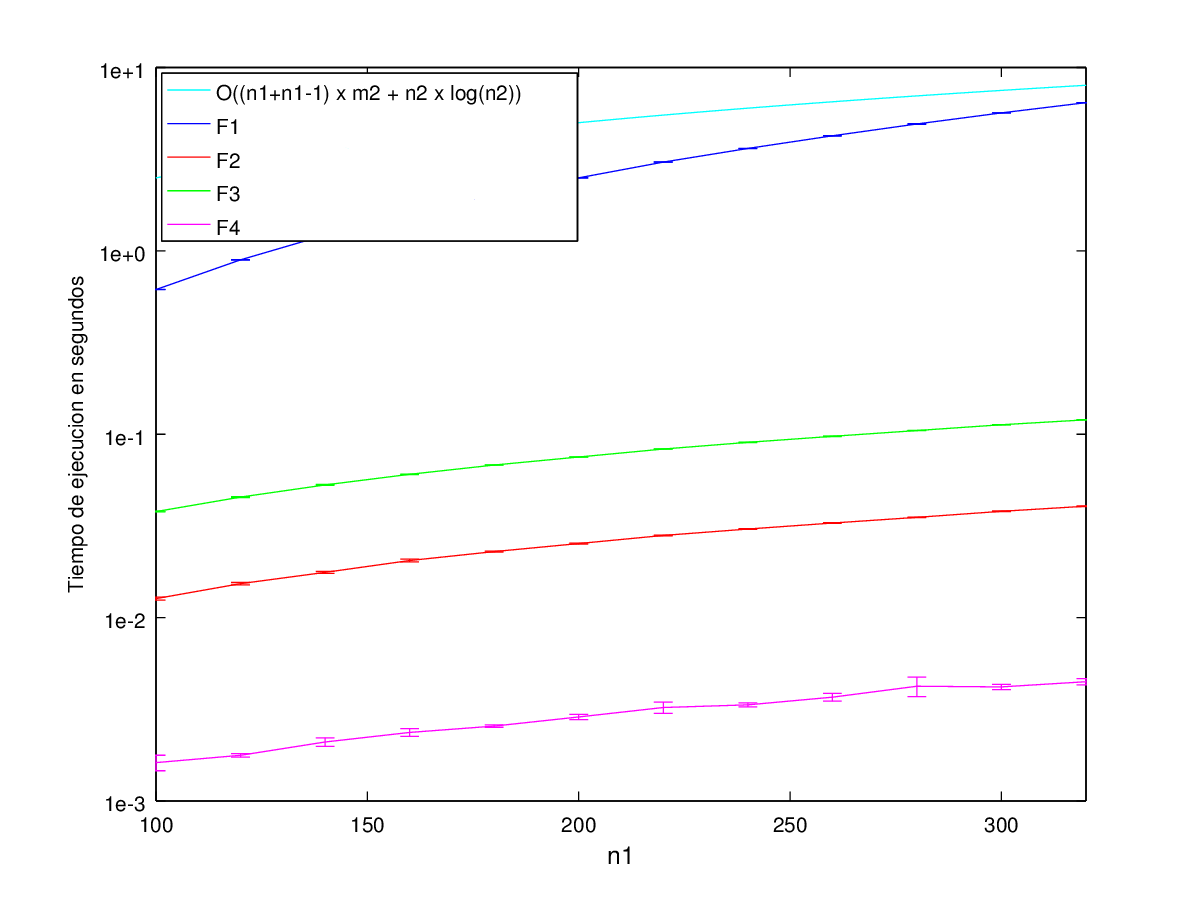
\includegraphics[height=10cm]{graficos/ejercicio4-exp2.png}
       \caption{Experimento 2}
	\end{figure}
        
     	\subsubsection*{Conclusiones}\;
En el gráfico se observa como todas las funciones de tiempo están por debajo de la curva de complejidad asintótica calculada. Se puede ver también como la diferencia en la cantidad de aristas influye en el tiempo de cómputo aunque siempre manteniéndose por debajo de la complejidad asintótica predicha.\\
Concluimos entonces que variando la cantidad de nodos, el tiempo de ejecución se mantendrá en el orden de complejidad predicho independientemente de la cantidad de aristas.
    
    \subsubsection*{Experimento 3}\; 
    El objetivo de este experimento fue extraer conclusiones acerca de la variación en el tiempo de cómputo requerido por el algoritmo para distintos valores de $m$ y $n$ variando los dos grafos al mismo tiempo pero siempre manteniendo $n_1$ igual a $n_2$ y $m_1$ igual a $m_2$. \\
Para generar los grafos con estas cantidades de aristas y nodos se utilizó el mismo generador que en el experimento anterior. 
        
        \subsubsection*{Datos de entrada}\;
        \noindent Los valores de $n$ tomados fueron desde $100$ hasta $1200$. Para cada $n$ se utilizó $3 \times n$ como cantidad de aristas.\\
        Para generar los grafos de forma aleatoria se utilizó el generador-grafo-rapido.cpp que se encuentra en la carpeta src y para correrlo se utilizó el exp3.sh que se encuentra en la carpeta exp/ejercicio4/exp3. \\
        Con el fin de acercarse a los valores reales y descartar posibles falsos resultados, se ejecuta la resolución del problema para cada una de los valores de $n$ cinco veces considerando luego el promedio entre los valores obtenidos pero graficando también el desvío estándar (la cantidad de repeticiones a realizar fue elegida arbitrariamente).\; 
 		\subsubsection*{Resultados}\;

    \begin{figure}[H]
      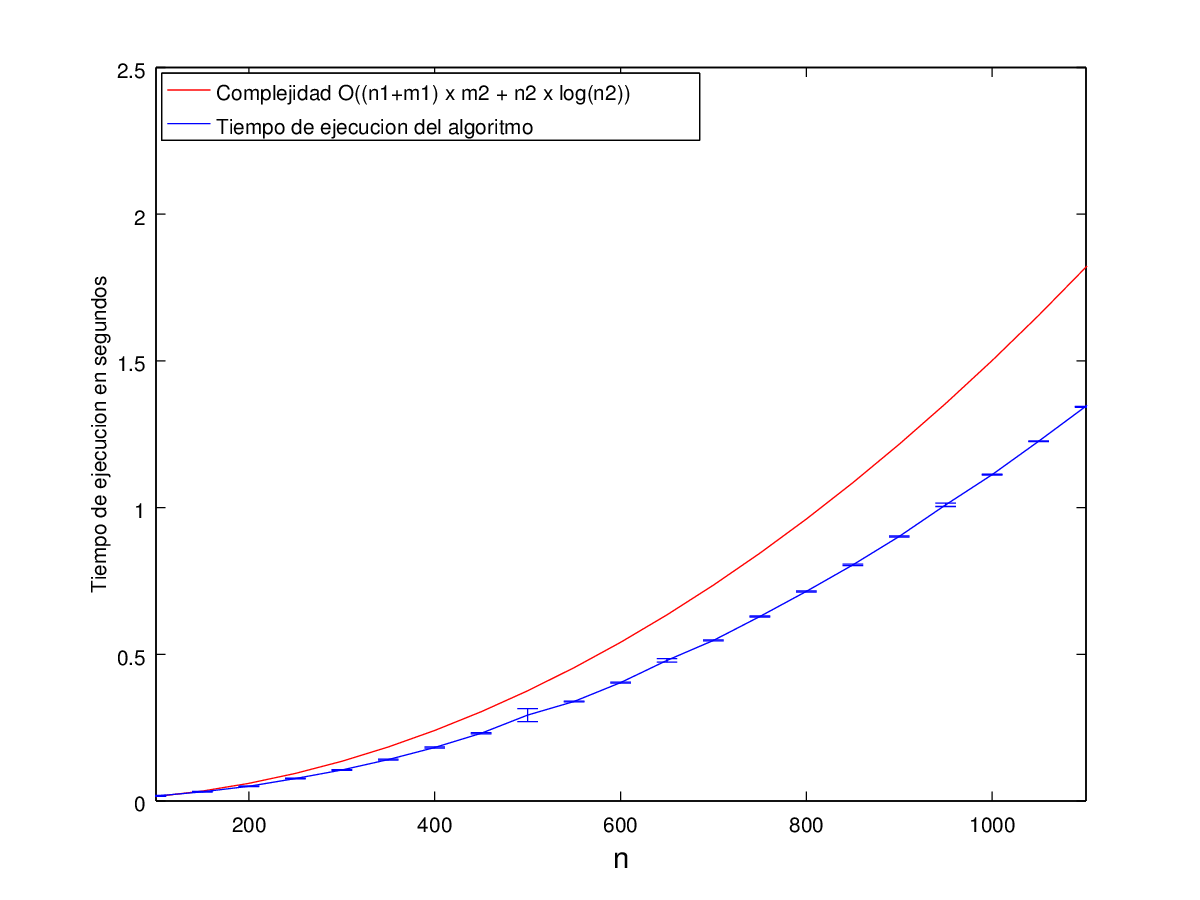
\includegraphics[height=10cm]{graficos/ejercicio4-exp3.png}
       \caption{Experimento 3}
	\end{figure}
        
     	\subsubsection*{Conclusiones}\;
Observamos en el gráfico que el comportamiento es el esperado, es decir que el tiempo de ejecución se mantiene por debajo del la complejidad temporal propuesta variando el $n_1=n_2$ y $m_1=m_2$.\\
    Concluimos que el algoritmo cumple con la complejidad propuesta anteriormente.
\clearpage
\section{Ejercicio 5}
\subsection{Introducción}
\noindent El objetivo de este ejercicio es resolver nuevamente el problema de MCS, pero esta vez con una heurística de búsqueda local, ya que suponemos que resolver el problema de forma exacta no se puede hacer en tiempo polinomial, pero sí podemos implementar un algoritmo heurístico que se ejecute eficientemente (tiempo polinomial) aunque no garantice la solución optima.
\subsection{Heurística}
\noindent Esta heurística se basa en moverse de una solución a otra solución vecina, es decir, a una solución similar a la anterior. Para ello es necesario determinar una función de vecindad para que dada una solución inicial, se la pueda modificar levemente dependiendo de algún criterio para obtener una nueva solución que supere a la anterior. Luego se repite este proceso hasta que no exista vecino de la solución actual que la supere.\\
El problema de este método es que se mueve a otra solución sólo si ésta es mejor que la anterior. Muchas veces sucede que para llegar a la solución óptima desde el resultado de partida es necesario pasar por algún resultado intermedio que genere menos aristas en el subgrafo común que el mejor obtenido hasta el momento. Como esta heurística no se mueve a soluciones intermedias peores puede pasar que el resultado no sea el óptimo real si no que sea un óptimo local, es decir, una solución óptima en una rama de soluciones cuando la mejor solución se encuentra en otro lado.

\subsubsection*{Vecindades}
\noindent En este ejercicio se analizarán dos criterios distintos para determinar cuando una solución es vecina de otra.
El algoritmo recibe dos grafos y se quiere hallar al máximo común subgrafo entre ellos. Sea $G1$ el que tiene la menor cantidad de nodos y $G2$ el otro. Si ambos tienen igual cantidad de nodos es indistinto cuál es $G1$ y cuál es $G2$.\\
Sea el vector mapeo el mismo que en el ejercicio 2.\\
\noindent Luego, dado un mapeo, se busca cuál es el conjunto de aristas que tienen en común ambos grafos renombrando cada nodo $i$ de $G1$ como $mapeo[i]$, es decir, el nodo que antes era el nodo $i$ ahora se llamará $mapeo[i]$.\\
Lo que queremos hallar es el mapeo para el cual la cantidad de aristas comunes entre los grafos sea la máxima posible ya que se sabe que la cantidad de nodos del máximo subgrafo común coincide con la cantidad de nodos de $G1$. \\

\noindent Sea $mapeo$ el vector de mapeo al que se le quiere buscar los vecinos y $mapeoVecino$ un vector de mapeo vecino de mapeo.


\subsubsection*{Vecindad tipo 1}
\noindent Dado un mapeo, un mapeo vecino válido es aquel que cumple con alguna de las siguientes condiciones:
\begin{itemize}
	\item Es igual que $mapeo$ pero tiene únicamente dos posiciones intercambiadas ($mapeoVecino[i] = mapeo[j]$ y $mapeoVecino[j] = mapeo[i]$ con $i \neq j$).
    \item Para alguna posición del vector mapeo se modifica el valor por otro que corresponde a un nodo de $G2$ que no estaba siendo utilizado en el vector anterior ($mapeoVecino[i]$ = $j$, con $ 0 \leq j$ $<$ $cantidad$ $de$ $nodos$ $de$ $G2$  y $j$ $\neq$ $mapeo[k]$ $\forall$ $0 \leq k <$ $cantidad$ $de$ $nodos$ $de$ $G1$).
\end{itemize}
\subsubsection*{Vecindad tipo 2}
\noindent Dado un mapeo, un mapeo vecino válido es aquel que cumple con alguna de las siguientes condiciones:
\begin{itemize}
	\item Es igual que $mapeo$ pero tiene únicamente tres posiciones intercambiadas ($mapeoVecino[i] = mapeo[j]$, $mapeoVecino[j] = mapeo[k]$ y $mapeoVecino[k] = mapeo[i]$, con $i \neq j \neq k$).
    \item Para alguna posición del vector mapeo se modifica el valor por otro que corresponde a un nodo de $G2$ que no estaba siendo utilizado en el vector anterior ($mapeoVecino[i]$ = $j$, con $ 0 \leq j$ $<$ $cantidad$ $de$ $nodos$ $de$ $G2$  y $j$ $\neq$ $mapeo[k]$ $\forall$ $0 \leq k <$ $cantidad$ $de$ $nodos$ $de$ $G1$).  
\end{itemize}

\subsection{Implementación}
\begin{algoritmo}{MCSbusquedaLocalUno}{vector(int) mapeo, vector(vector(int)) grafoChico, vector(vector(int)) grafoGrande}{vector(int)}

	\tipo{vector(vector(int))} vecindadA = calcularVecindadTipoA(mapeo);\com*{En vecindadA se tiene el conjunto de mapeos vecinos a mapeo que cumplen con el primer criterio de alguna de las vecindades mencionado en la sección vecindades} 
    \tipo{vector(vector(int))} vecindadB = calcularVecindadTipoB(mapeo, grafoGrande.size());\com*{En vecindadB se tiene el conjunto de mapeos vecinos a mapeo que cumplen con el segundo criterio de alguna de las vecindades mencionado en la sección vecindades} 
    \tipo{vector(int)} mapeoNuevo = dameElMejorVecinoDelMapeoActual(vecindadA, vecindadB, mapeo, grafoChico, grafoGrande);\com*{En mapeoNuevo tengo el mejor mapeo vecino al mepeo actual} 
     
     \While{ExisteVecinoDeLaSolucionActualQueLaSupere(mapeo)}{
		mapeoNuevo = dameElMejorVecinoDelMapeoActualOMejorActual(vecindadA, vecindadB, mapeo, grafoChico, grafoGrande);	\com*{Devuelve el mejor entre todas los los mapeos vecinos. En caso de que no haya uno mejor devuelve el mapeo actual} 
        \If{(noSonIguales(mapeo, mapeoNuevo))}{
       		mapeo = mapeoNuevo
        	vecindadA = calcularVecindadDosTipoA(mapeo);
			vecindadB = calcularVecindadTipoB(mapeo, grafoGrande.size());
      	}
  }
        
\end{algoritmo}
\subsubsection*{Correctitud}
\noindent Veamos ahora que el resultado final es un subgrafo. El grafo inicial es subgrafo ya que iniciamos con un mapeo que devuelve el algoritmo de heurística golosa y, como demostramos antes, es un mapeo que genera un subgrafo válido. Luego lo que hace la heurística es moverse a una solución vecina, lo que genera un nuevo mapeo. Veamos ahora que para cualquiera de las vecindades este mapeo sigue siendo válido: 
\begin{itemize}
	\item Cuando sólo cambio dos o tres de lugar el mapeo no puede pasar a ser inválido ya que todos los nodos de $G1$ siguen estando mapeados con otros nodos de $G2$, lo único que se cambió fue con qué nodo se encuentra mapeado cada uno de los que se modificó.
    \item Cuando se cambia el valor de uno por otro que no estaba siendo utilizado, sigue siendo un mapeo válido ya que para todos los nodos que no se modificó el mapeo sigue siendo lo mismo, y el nodo modificado está mapeado con uno que no estaba siendo utilizado y que pertenece a los nodos de $G2$. Entonces el mapeo sigue siendo válido. 
\end{itemize}
Entonces cuando busco los vecinos de un mapeo aplicando cualquiera de las dos vecindades vuelvo a obtener un mapeo válido. Si vuelvo a aplicar tantas veces como sea necesario hasta que no exista vecino de la solución actual que la supere, como cada vez que lo aplico parto de un mapeo válido (porque, o es la primera vez que parto del goloso o es el resultado de aplicarle a un mapeo válido la vecindad) entonces el mapeo final es un mapeo válido. \\
Luego lo que se hace con este mapeo es buscar las aristas que tienen en común ambos grafos, por lo tanto la respuesta es un subgrafo de ambos grafos. 


\subsection{Complejidad}
Para analizar la complejidad de este algoritmo, en primer lugar veremos que para ambos tipos de vecindades la complejidad es la misma. Esto es así pues la 2-vecindades y las 3-vecindades son generadas de la misma forma con la única salvedad de que en vez de seleccionar 2 elementos a intercambiar se seleccionan 3 y se hacen los intercambios de manera aleatoria pero inmediata (igual que en el primer caso). Como consecuencia de ésto, las complejidades son las mismas ya que lo que era $\mathcal{O}(1)$ en el algoritmo de las 2-vecindades seguirá siéndolo en el de las 3-vecindades.\\
Nuevamente asumimos G1 el mas pequeño de los grafos en cuanto a la cantidad de nodos.\\
Es por esto que para simplificar el análisis, estudiaremos la complejidad del algoritmo de vecindades tipo 1 (2-vecindades) y podremos concluir que el mismo análisis será válido para el de las 3-vecindades exceptuando constantes que resultan irrelevantes en cuanto al orden de complejidad.\\
El algoritmo con las vecindades tipo 1 será:
\begin{enumerate}
\item Construir el mapeo inicial con el algoritmo goloso (cuya complejidad es $\mathcal{O}((n_1+m_1)*m_2+n_2*log(n_2))$ , como ya analizamos en el Ej.4).
\item Llamar a la búsqueda local para mejorar el mapeo (esto es lo que aún no tiene calculada la complejidad).
\item Calcular las aristas del nuevo mapeo (esto ya está calculado en Ej.2 y en Ej.4, es $\mathcal{O}((n_1+m_1)*m_2) $).
\end{enumerate}
 Calcularemos entonces el inciso 2, es decir, la búsqueda local.
 Esta búsqueda local consta de:
 \begin{itemize}
 \item Construir vecindades ``tipo a'' es construir las vecindades de intercambiar 2 elementos dentro del mapeo vigente. Estos resultan ser $n_1$ vectores de tamaño $n_1$ que se recorren una cantidad constante de veces, sobre los cuales se hacen operaciones y comparaciones $\mathcal{O}(1)$, por lo que la complejidad total de esto es $\mathcal{O}(n_1^2)$.
 \item Construir vecindades ``tipo b''. Estas constan de intercambiar un vértice de la imagen del mapeo vigente con un vértice que no está en el mapeo vigente. También tiene complejidad $\mathcal{O}(n_1^2)$ pues lo que se hace en definitiva es generar $n_1$ vectores de tamaño $n_1$ creados de la siguiente forma: sobre el mapeo original (que tiene tamaño $n_1$) recorrer para elegir el primero a reemplazar, y luego para elegir el segundo, elegir alguno que no esté en el mapeo (esto es $\mathcal{O}(n_1)$). Por lo que la complejidad total de ésto sería $\mathcal{O}(n_1^2)$.
 \item El próximo paso es tomar el mejor mapeo, tanto de la vencidad-a como la vecindad-b. Para esto se tiene que ver para cada uno de los $2*n_1$ mapeos ($n_1$ de ``a'' y $n_1$ de ``b'' ) la cantidad de aristas que se pueden encontrar en común, usando el algoritmo ya usado en el Ej.2 y el Ej.4 con complejidad $\mathcal{O}((n_1+m_1)*m_2)$. Como se usa $\mathcal{O}(n_1)$ veces, la complejidad de seleccionar el mejor mapeo de las vecindades sera de $\mathcal{O}((n_1+m_1)*m_2*n_1)$.
\end{itemize}
La complejidad de este proceso resulta $\mathcal{O}((n_1+m_1)*m_2*n_1)$ ya que es la complejidad del tercer ítem y absorbe la complejidad $\mathcal{O}(n_1^2)$ de los 2 primeros.\\
Todo este proceso se realiza mientras que la cantidad de aristas del nuevo mapeo adquirido sea mayor. Una vez que se estanca, es decir, que no se encuentra en las vecindades algún mapeo que haga crecer la cantidad de aristas, el algoritmo termina. Es decir que para que se itere una vez más todo el procedimiento dictado, la cantidad de aristas en el nuevo (grafo isomorfo a) subgrafo debe aumentar por lo menos en 1.\\
En el peor caso empezaría en 0 la cantidad de aristas, y en cada iteración aumentaría en 1 hasta llegar como máximo al min\{$m_1,m_2$\} pues un subgrafo común no puede tener mas aristas que ninguno de los dos grafos.\\
Es decir que este procedimiento se repetirá a lo sumo min\{$m_1,m_2$\} veces dando a toda la búsqueda local (inciso 2.) una complejidad en el peor caso de $\mathcal{O}((n_1+m_1)*m_2*n_1*min\{m_1,m_2\})$.\\
Esta complejidad sumada a la de construir el mapeo inicial con el algoritmo goloso (inciso 1.) de $\mathcal{O}((n_1+m_1)*m_2+n_2*log(n_2))$ dará la complejidad total del algoritmo que será: \\
$\mathcal{O}((n_1+m_1)*m_2*n_1*min\{m_1,m_2\}+n_2*log(n_2))$.



\subsection{Experimentación}
\noindent El algoritmo toma dos grafos para calcular el máximo subgrafo común. Para tomar las mediciones y determinar el tiempo de cómputo de la heurística, generalmente, se modificarán únicamente las cantidades de nodos y aristas de sólo uno de ésos grafos. \\
Sea $n_1$ y $m_1$ la cantidad de nodos y aristas del grafo que se modificará para tomar las mediciones respectivamente y $n_2$, $m_2$ la cantidad de nodos y aristas del grafo al que se le dejarán constantes las cantidades de nodos y aristas, aunque en cada caso podrán utilizarse grafos distintos pero con la misma cantidad de vértices y de aristas.
    
\subsubsection*{Experimento 1}\;
\noindent El objetivo de este experimento fue extraer conclusiones acerca de la variación en el tiempo de cómputo requerido por el algoritmo para cada una de las vecindades para distintos valores de $m_1$, con el fin de determinar su complejidad, dejando $n_1$ fijo. \\
   Para ello se utiliza un generador de grafos que funciona de la siguiente manera: dada una cantidad de nodos y aristas, en cada paso crea una nueva arista con extremos válidos, es decir, entre 0 y la cantidad de nodos - 1, y que no esté repetida (que no haya sido creada todavía).\\
   Este experimento se realiza de la misma manera utilizando primero la vecindad tipo 1 y luego la vecindad tipo 2.
     	
\subsubsection*{Datos de entrada}\;
 \noindent Para correr el algoritmo con poda los valores de $m_1$ tomados fueron desde $0$ hasta $350$ de $30$ en $30$. El valor de $n_1$ fue $150$. Los valores de $n_2$ y $m_2$ fueron $150$ y $200$ respectivamente. El valor de $cuantosVecinosMiro$ fue $20$. Estos valores fueron elegidos de forma arbitraria.\\
        Para generar los grafos de forma aleatoria se utilizó el generador-grafo-rapido.cpp que se encuentra en la carpeta src y para correrlo se utilizó el exp1.sh que se encuentra en la carpeta exp/ejercicio5/exp1. \\
        Con el fin de acercarse a los valores reales y descartar posibles falsos resultados, se ejecuta la resolución del problema para cada una de los valores de $m_1$ cinco veces considerando luego el promedio entre los valores obtenidos pero graficando también el desvío estándar (la cantidad de repeticiones a realizar fue elegida arbitrariamente).\; 
     	
\subsubsection*{Resultados}\;

    \begin{figure}[H]
      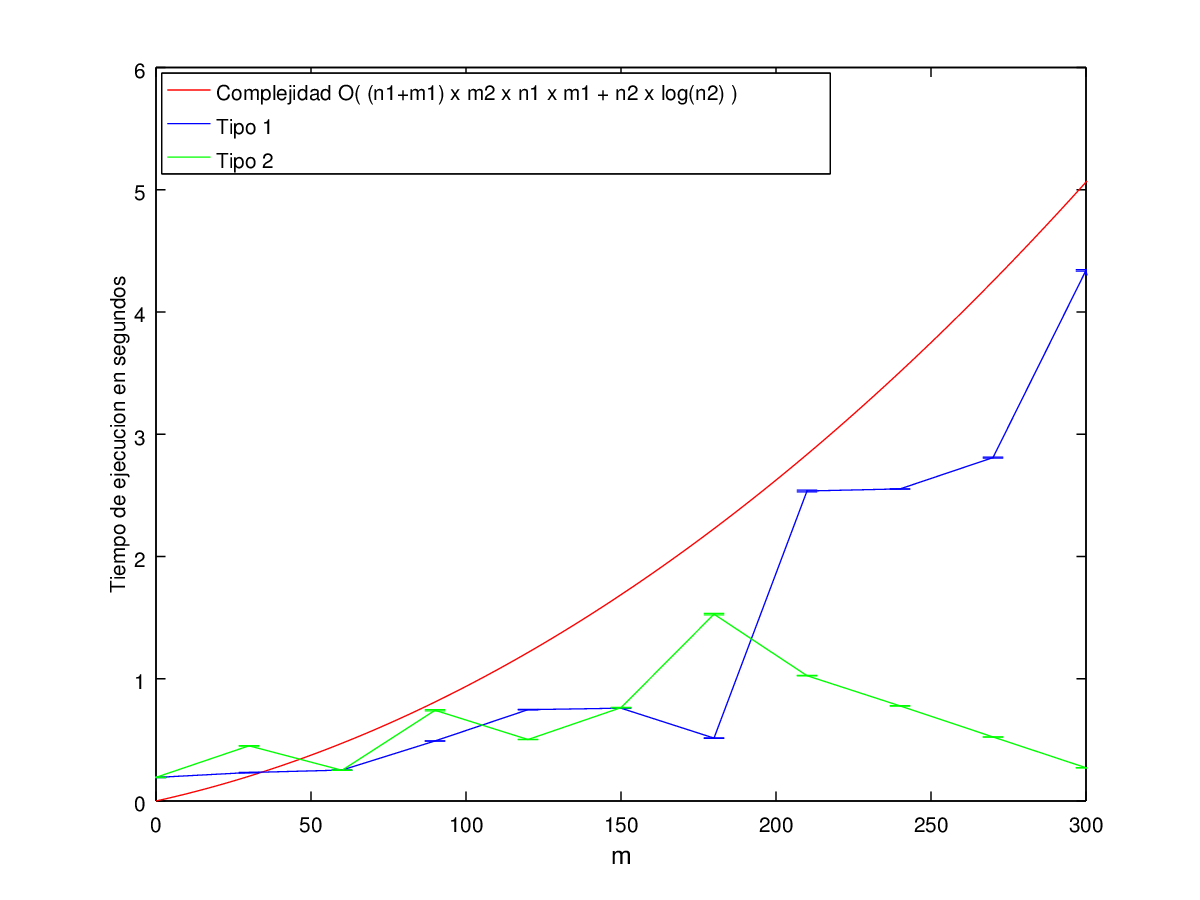
\includegraphics[height=10cm]{graficos/ejercicio5-exp1.png}
       \caption{Experimento 1}
	\end{figure}
    
\subsubsection*{Conclusiones}\;
 Notamos en el gráfico que en ambos casos los tiempos de ejecución de los algoritmos (uno de cada vecindad) están por debajo de la curva de complejidad predicha.\\
 Concluimos que se respeta la complejidad propuesta para el caso de variar el $m_1$.\\
 Adicionalmente notamos que para el algoritmo de vecindad tipo 2, en ciertas instancias de m grande parece tardar menos. Esto podría ser probablemente por un estancamiento rápido en un máximo local (o un casual rápido encuentro de una solución muy buena).\\
 Esta última proposición la volveremos a analizar cuando estudiemos la calidad de las soluciones.
        
        
\subsubsection*{Experimento 2}\;
\noindent Este experimento es similar al anterior, pero ahora se va a variar la cantidad de nodos. Para ello, para cada cantidad de nodos se definirá una función para determinar la cantidad de aristas que tendrá el grafo. \\
\noindent Se tuvieron en cuenta 4 funciones, con el fin de que el grafo obtenido no sea siempre uno especial y de esta forma poder analizar diferentes casos. 
        \begin{itemize}
        \item F1($n_1$) = $n_1$($n_1$-1))/2 = $m_1$ 
        \item F2($n_1$) = $n_1$-1 = $m_1$ 
        \item F3($n_1$) = 3$n_1$
        \item F4($n_1$) = $n_1^{2}$/10
		\end{itemize} 
Para generar los grafos con estas cantidades de aristas y nodos se utilizó el mismo generador que en el experimento anterior.
Este experimento se realiza utilizando primero la vecindad tipo 1 y luego la vecindad tipo 2.
\subsubsection*{Datos de entrada}\;
    \noindent Los valores de $n_1$ tomados fueron desde $10$ hasta $70$ de $5$ en $5$. \\
       Los valores de $n_2$ y $m_2$ fueron $50$ y $200$ respectivamente. El valor de $cuantosVecinosMiro$ fue $20$. Estos valores fueron elegidos de forma arbitraria \\
        Para generar los grafos de forma aleatoria se utilizó el generador-grafo-rapido.cpp que se encuentra en la carpeta src y para correrlo se utilizó el exp2.sh que se encuentra en la carpeta exp/ejercicio5/exp2. \\
        Con el fin de acercarse a los valores reales y descartar posibles falsos resultados, se ejecuta la resolución del problema para cada una de los valores de $n_1$ cinco veces considerando luego el promedio entre los valores obtenidos pero graficando también el desvío estándar (la cantidad de repeticiones a realizar fue elegida arbitrariamente).\; 
\subsubsection*{Resultados}\;

    \begin{figure}[H]
      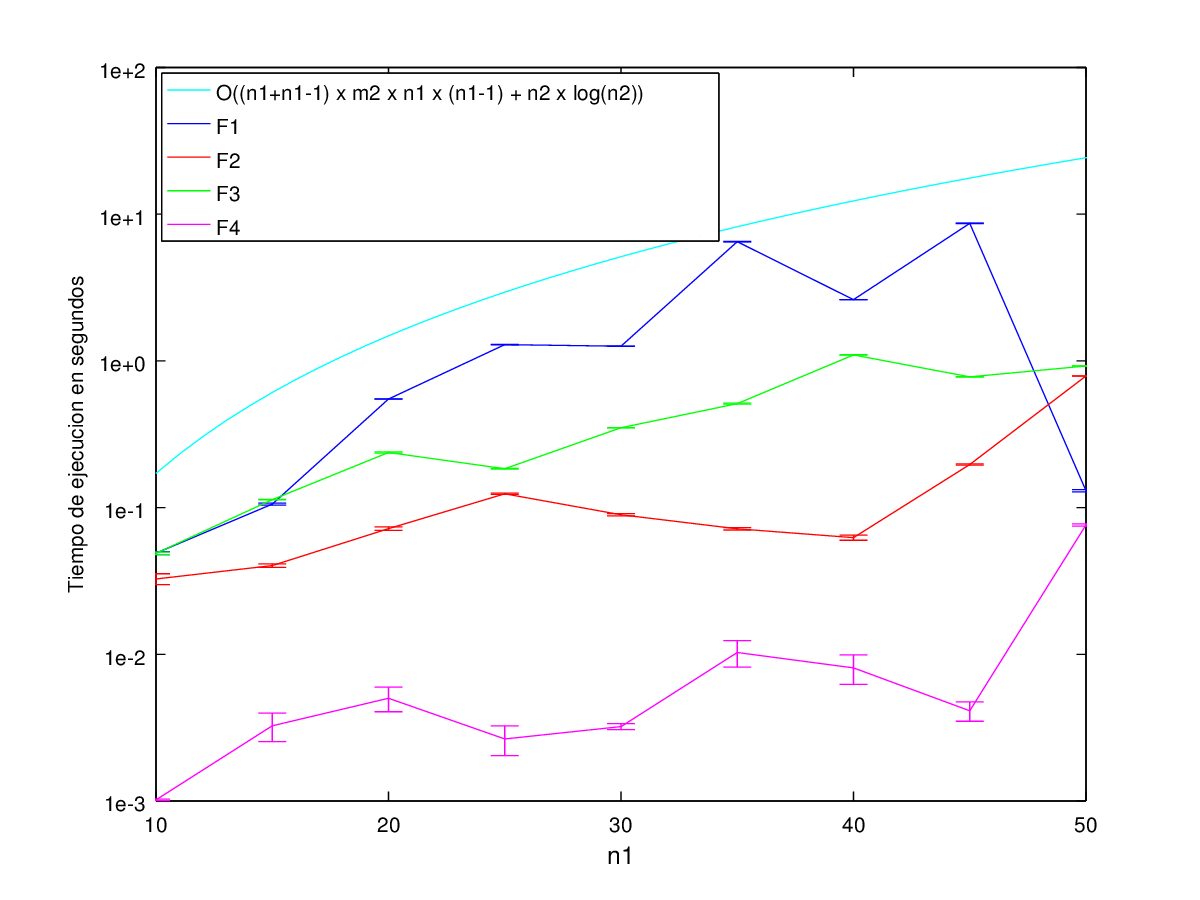
\includegraphics[height=8cm]{graficos/ejercicio5-exp2-tipo1.png}
       \caption{Experimento 2 - Tipo 1}
	\end{figure}
    
        \begin{figure}[H]
      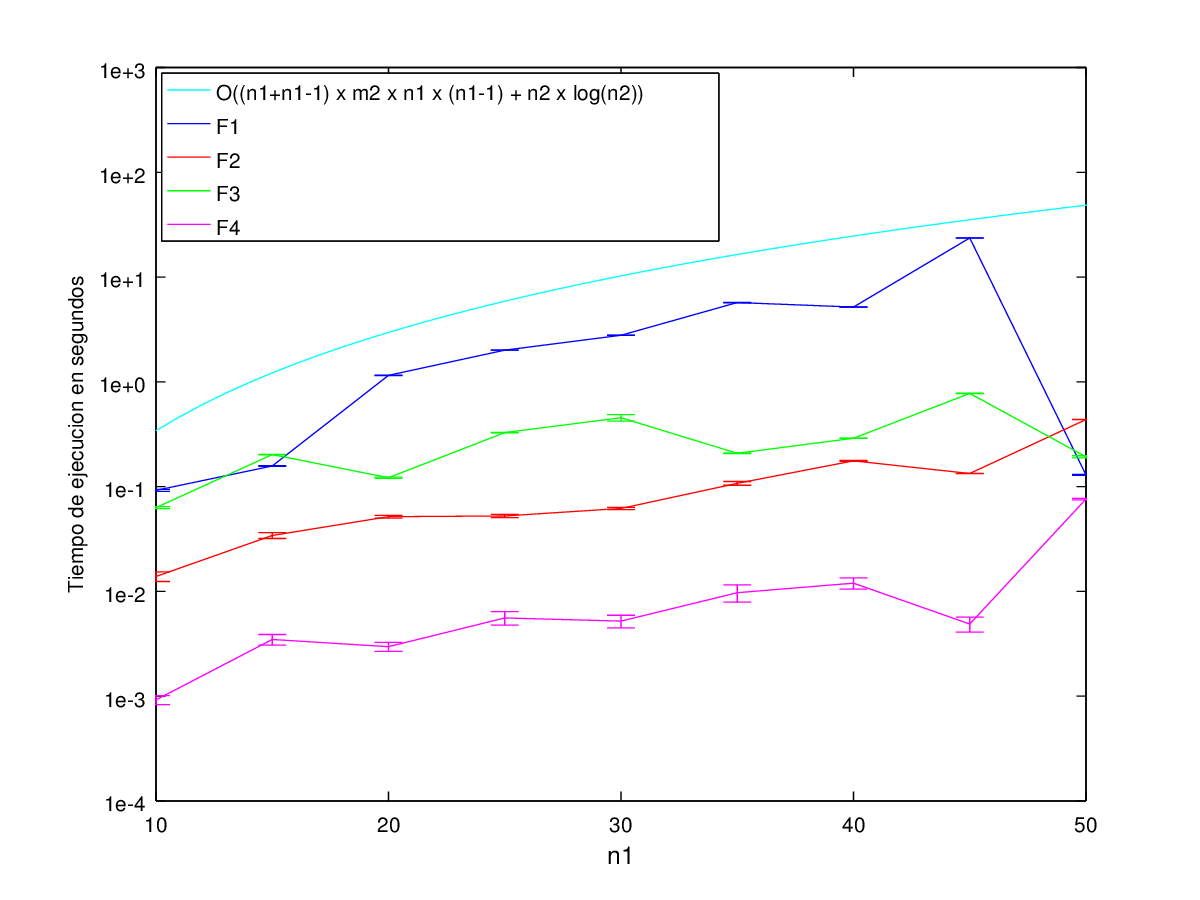
\includegraphics[height=8cm]{graficos/ejercicio5-exp2-tipo2.png}
       \caption{Experimento 2 - Tipo 2}
	\end{figure}
     	
\subsubsection*{Conclusiones}\;
 Se observa en ambos gráficos que se respeta la cota de complejidad prefijada en todos los casos, esto nos lleva a concluir que la cota efectivamente se cumple.\\
 Además puede apreciarse que el desarrollo es similar para ambas vecindades y que ambos algoritmos están dentro del mismo rango en tiempo de cómputo.\\
 También puede apreciarse que los casos de éxito (los casos donde el algoritmo tarda menos) son los mismos, dado que el orden en tiempo de cómputo es el mismo en ambos gráficos, es decir, F1 es el mas lento, seguido de F3, F2 y F4 en ese orden para ambos algoritmos (en ambos grafos es el mismo orden).\\
 Concluimos de este experimento entonces:\\
 \begin{itemize}
\item Se respeta la cota de complejidad propuesta en ambos algoritmos.
\item Los casos de mayor eficiencia en una y en otra vecindad son los mismos.
\end{itemize}
\subsubsection*{Experimento 3}\; 
    El objetivo de este experimento fue extraer conclusiones acerca de la variación en el tiempo de cómputo requerido por el algoritmo para distintos valores de $m$ y $n$ variando los dos grafos al mismo tiempo pero siempre manteniendo $n_1$ igual a $n_2$ y $m_1$ igual a $m_2$. \\
Para generar los grafos con estas cantidades de aristas y nodos se utilizó el mismo generador que en el experimento anterior. 
Este experimento se realiza utilizando primero la vecindad tipo uno y luego la vecindad tipo 2.
        
\subsubsection*{Datos de entrada}\;
    \noindent Los valores de $n$ tomados fueron desde $10$ hasta $70$ de $5$ en $5$. El valor de $cuantosVecinosMiro$ fue $20$. Estos valores fueron elegidos de forma arbitraria. \\
        Para generar los grafos de forma aleatoria se utilizó el generador-grafo-rapido.cpp que se encuentra en la carpeta src y para correrlo se utilizó el exp3.sh que se encuentra en la carpeta exp/ejercicio5/exp3. \\
        Con el fin de acercarse a los valores reales y descartar posibles falsos resultados, se ejecuta la resolución del problema para cada una de los valores de $n$ cinco veces considerando luego el promedio entre los valores obtenidos pero graficando también el desvío estándar (la cantidad de repeticiones a realizar fue elegida arbitrariamente).\; 
\subsubsection*{Resultados}\;

    \begin{figure}[H]
      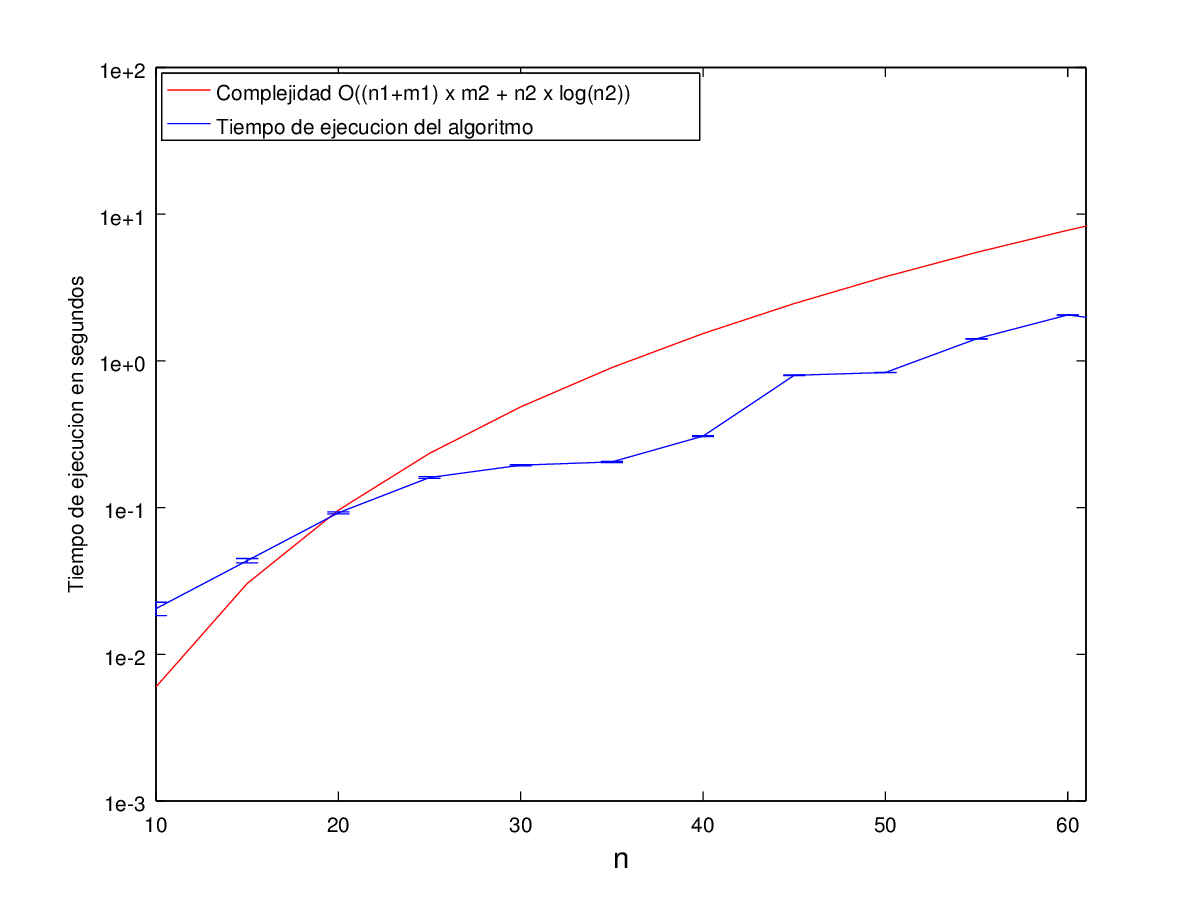
\includegraphics[height=8cm]{graficos/ejercicio5-exp3-tipo1.png}
       \caption{Experimento 3 - Tipo 1}
	\end{figure}
    
        \begin{figure}[H]
      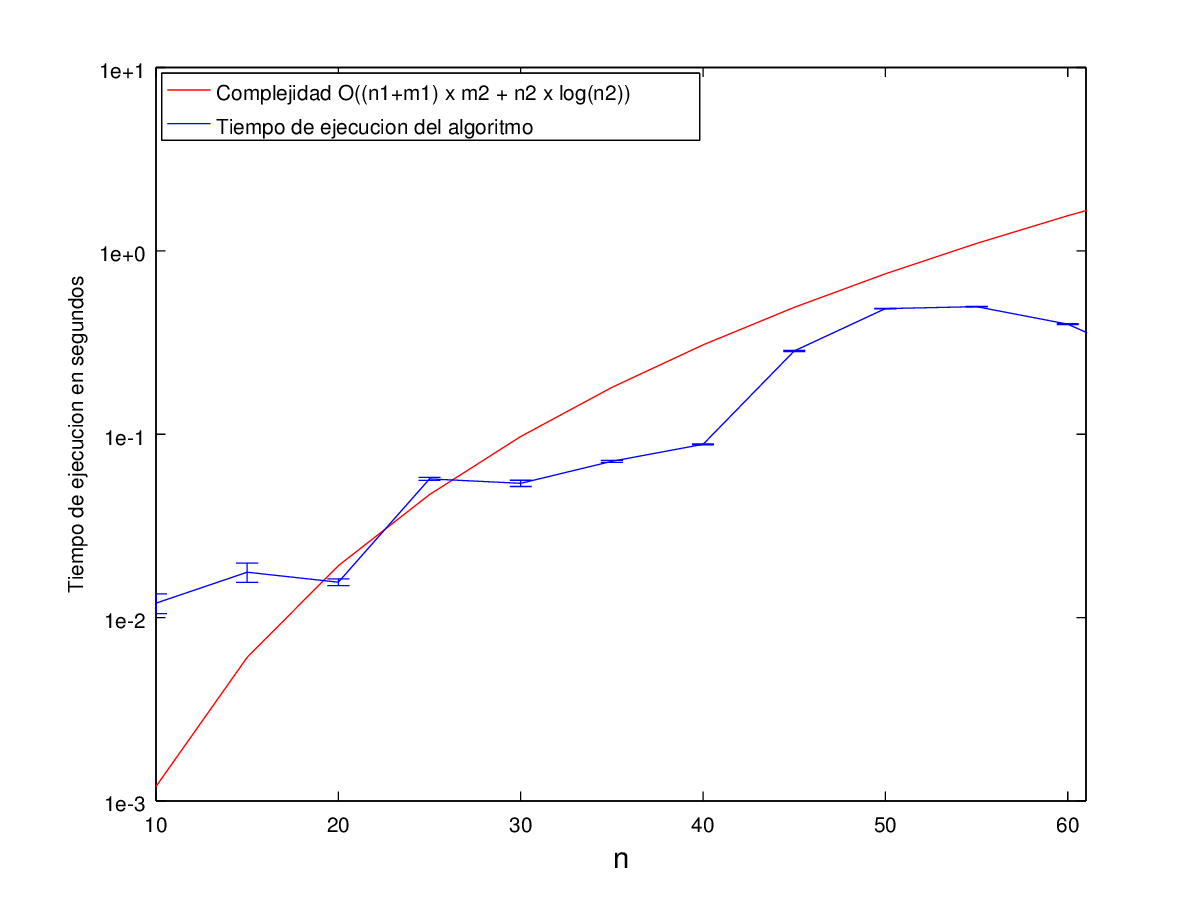
\includegraphics[height=8cm]{graficos/ejercicio5-exp3-tipo2.png}
       \caption{Experimento 3 - Tipo 2}
	\end{figure}


\subsubsection*{Conclusiones}\;
    Se observa y se concluye de este experimento que se respeta la cota de complejidad propuesta en ambos algoritmos, ya que la curva de tiempo de cómputo se sitúa por debajo de la del orden de complejidad.

\subsubsection*{Experimento 4}\;
\noindent El objetivo de este experimento fue comparar los diferentes tipos de vecindades. Para  ello compararemos sobre grafos al azar (variando su tamaño) los tiempos de ejecución por un lado en un gráfico y por otro lado graficaremos la cantidad de aristas de la solución de cada algoritmo (uno de cada vecindad) para así comparar la calidad de las soluciones. \\
Para ello se utiliza el mismo generador que en el experimento 1.\\
Para realizar este experimento se ejecutarán las dos vecindades pasándoles por parámetro de entrada los mismos grafos para poder realizar una comparación más exacta. \\

\subsubsection*{Datos de entrada}\;
    \noindent Los valores de $n_1$ tomados fueron desde $10$ hasta $70$ de $5$ en $5$. \\
       Los valores de $n_2$ y $m_2$ fueron $200$ y $2500$ respectivamente. El valor de $cuantosVecinosMiro$ fue $20$. Estos valores fueron elegidos de forma arbitraria. \\
        Para generar los grafos de forma aleatoria se utilizó el generador-grafo-rapido.cpp que se encuentra en la carpeta src y para correrlo se utilizó el exp4.sh que se encuentra en la carpeta exp/ejercicio5/exp4. \\
        Con el fin de acercarse a los valores reales y descartar posibles falsos resultados, se ejecuta la resolución del problema para cada una de los valores de $n_1$ cinco veces considerando luego el promedio entre los valores obtenidos pero graficando también el desvío estándar (la cantidad de repeticiones a realizar fue elegida arbitrariamente).\; 

\subsubsection*{Resultados}\;

    \begin{figure}[H]
      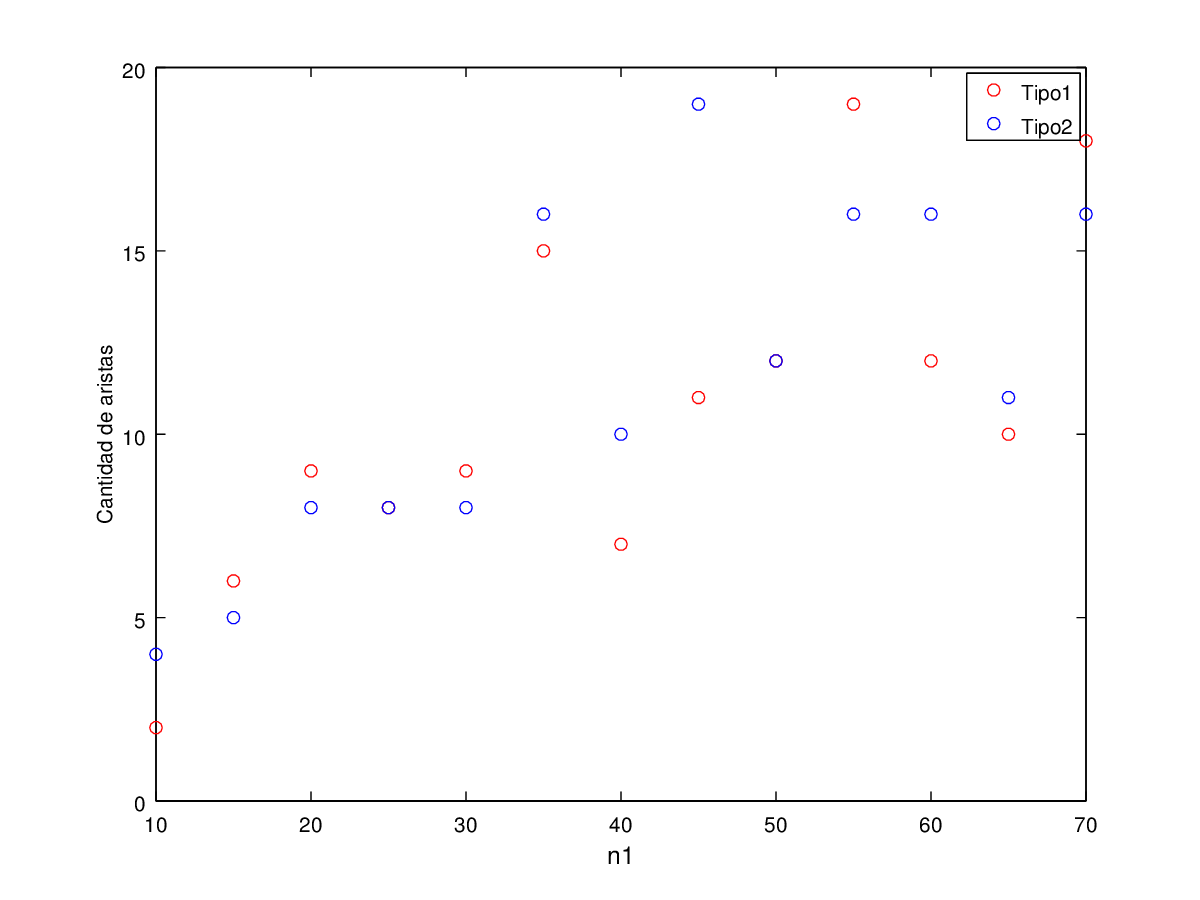
\includegraphics[height=8cm]{graficos/ejercicio5-exp4aristas.png}
       \caption{Experimento 4 - Aristas}
	\end{figure}
    
        \begin{figure}[H]
      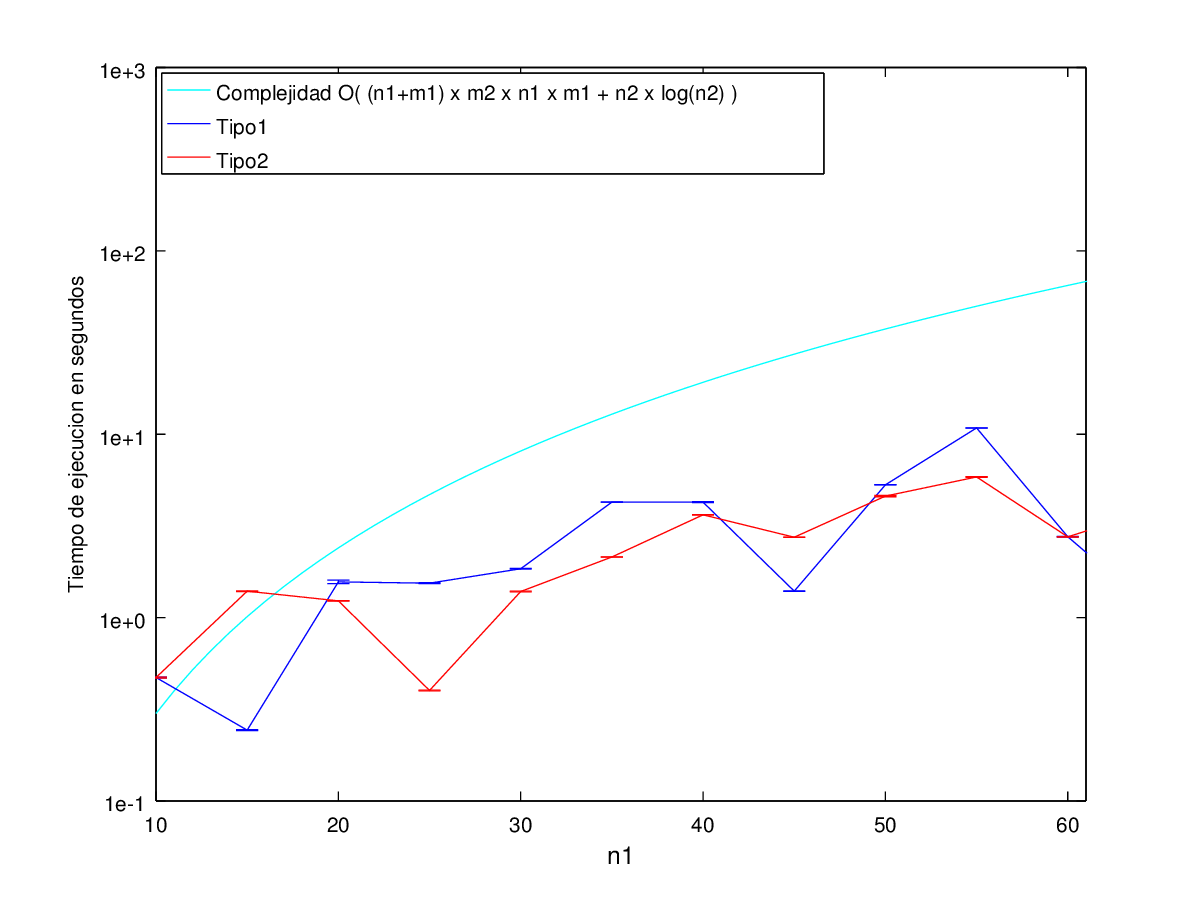
\includegraphics[height=8cm]{graficos/ejercicio5-exp4tiempos.png}
       \caption{Experimento 4 - Tiempos}
	\end{figure}
     	
\subsubsection*{Conclusiones}\;

 \noindent Del primer gráfico (el de la cantidad de aristas por solución), se puede observar una dispersión bastante uniforme, tal vez podría decirse que las vecindades tipo 1 son ligeramente más efectivas en encontrar mejores soluciones (en una gran cantidad de casos), aunque también hay casos en los que se prueba ser mejor elegir vecindades tipo 2.\\
    En los tiempos se observa que ambos cumplen la cota de complejidad predicha, pero no se observa que alguno sea más eficiente que el otro, es decir, son similares en el tiempo de cómputo ambos algoritmos con sus distintas vecindades.\\
    Concluimos entonces que es ligeramente mejor el algoritmo que aplica vecindades tipo 1 ya que es ligeramente mejor en cantidad de aristas y en tiempos, ambos algoritmos son muy similares.
\clearpage
\section{Ejercicio 6}

\subsection{Introducción}
\noindent El objetivo de este ejercicio es resolver nuevamente el problema de MCS, pero esta vez con una metaheurística de búsqueda tabú, ya que suponemos que resolver el problema de forma exacta no se puede hacer en tiempo polinomial, pero sí podemos implementar un algoritmo heurístico que se ejecute eficientemente (tiempo polinomial) aunque no garantice la solución óptima.
\subsection{Metaheurística}
\noindent La búsqueda tabú es una metaheurística que al igual que búsqueda local busca pasar de una solución a otra e intenta corregir el problema del estancamiento en óptimos locales, es decir, que no se quede iterando siempre en una rama de soluciones cuando podría haber una solución mejor en otro lado. Para solucionar este problema, búsqueda tabú permite pasar de una solución a otra por más de que la segunda no sea mejor. Esto puede llevar a que el algoritmo se quede ciclando dentro de las mismas soluciones siempre. Por ejemplo, dado S óptimo local y S' mejor solución vecina de S y también S mejor solución vecina de S' pasaríamos de S a S' y luego de nuevo a S y así seguiríamos ciclando. Para solucionar esto se implementará una lista tabú la cual contendrá las últimas soluciones tomadas de forma que no pueda volver a repetirlas. Si sólo mantuviéramos la última solución podría pasar que el ciclo fuera entre 3 o más soluciones. Luego mencionaremos otras formas de implementar tabú search sin guardar soluciones enteras. Dejar muchas soluciones se basa en la idea de que al alejarse lo suficiente de una solución es muy poco probable que se vuelva a la misma. La cantidad de soluciones a dejar dentro de la lista tabú es un punto a analizar en este ejercicio. No sólo está el problema de la memoria que ocuparía guardar todas las soluciones ya visitadas si no que también al tener demasiadas soluciones guardadas, cada vez que se quiera mirar si una solución nueva posible se encuentra o no en la lista tabú se perdería muchísimo tiempo revisando una por una las soluciones que se encuentran guardadas y comparando con la nueva a ver si coincide. 

\subsubsection*{Vecindades}
\noindent En este ejercicio se analizarán dos criterios distintos para determinar cuando una solución es vecina de otra.
Las vecindades a utilizar son las mismas que las utilizadas en el ejercicio 5. 

\subsubsection*{Variaciones de búsqueda tabú}
\noindent Para la metaheurística de búsqueda tabú existen variaciones en diferentes aspectos del algoritmo. Por ejemplo, en la lista tabú se podrían guardar en lugar de soluciones ya visitadas, movimientos hechos para no repetirlos o características de las soluciones que no debería repetir. Otro de los aspectos que se pueden variar son los criterios de terminación, es decir, cuándo se considera que ya se iteró sobre la suficiente cantidad de vecinos y el resultado ya debería ser, en la mayoría de los casos, muy próximo a la solución real. Algunos ejemplos de los criterios que se pueden utilizar son:
\begin{itemize}
    \item No se encontró una mejora en las últimas k iteraciones.
	\item Se alcanzó un límite prefijado de k iteraciones.
	\item Se alcanzó un límite prefijado de tiempo.
    \item Se obtuvo una solución cercana a una cierta cota conocida.
    \item En las últimas k iteraciones todas las soluciones fueron tabú.
\end{itemize}
También se puede variar el tamaño de la lista tabú. Como ya mencionamos antes no solo está el problema de la memoria que ocupa si no que también al tener demasiadas soluciones guardadas cada vez que se quiera mirar si una solución nueva posible se encuentra o no en la lista tabú se deberá revisar una por una las soluciones que se encuentran guardadas y compararlas con la nueva a ver si coincide, lo que puede ser muy costoso. \\
Además, si algún mapeo tiene demasiados vecinos, mirar todos y decidir cual es el mejor también es muy costoso, por lo que la cantidad de vecinos de un mapeo que se tendrá en cuenta también es un criterio que puede variar. \\
En el algoritmo planteado para resolver este ejercicio el criterio de parada que se utilizó fue parar cuando no se haya encontrado una mejora en las últimas k iteraciones, donde k es un parámetro que se recibirá por parámetro al igual que el tamaño máximo que puede tener la lista tabú y la cantidad de vecinos de un mapeo que se tendrá en cuenta para determinar el mejor vecino.\\
La cantidad de vecinos a tener en cuenta debe ser mayor que el tamaño máximo que puede tener la lista tabú. De esta forma nos aseguramos que seguro al menos uno de ellos no se encontrará en la lista tabú. En caso de que la cantidad de vecinos totales que tiene la solución actual sea menor que la cantidad de vecinos a tener en cuenta y menor al tamaño máximo que puede tener la lista tabú, podría pasar que todos los vecinos estén en la lista tabú. Como es un caso muy particular asumimos que no va a suceder nunca.

\subsection{Implementación}
\noindent La lista tabú se usa en dos ocasiones, una para ver si algo está o no en la lista tabú, y otra para actualizarla (agregar soluciones, y si se llenó sacar la más vieja). En cada iteración la consulto para cada vecino y la actualizo una sola vez. Entonces, para poder consultar la lista de forma rápida para ver si una solución está o no en la lista, se utilizará $set<vector<int>> tabuPorMapeo$ que busca soluciones en $O(log cantSoluciones * tamano de las soluciones)$. En esta estructura, saber cuál fue el primero agregado, es decir, el mapeo que debo sacar cuando la lista tabú llega a su tamaño máximo y se quiere consultar por un nuevo vecino, es complicado. Por lo tanto se tendrá en paralelo con el set, la información también en un $queue<vector<int> >$ tabuCola, que es una cola fifo. Luego, comparar soluciones es preguntarle al set si la tiene.

 \begin{algoritmo}{MCSTabu}{vector(int) mapeo, vector(vector(int)) grafoChico, vector(vector(int)) grafoGrande, int cuantosVecinosMiro, int maxTamTabu, int k}{vector(int)}
 
 	\tipo{vector(int)} mejorMapeo; \com*{En mejorMapeo guardamos el mapeo que genera la mayor cantidad de aristas entre los dos grafos} 
	mejorMapeo $\gets$ mapeo; 
	\tipo{vector(vector(int))} vecindadA = calcularVecindadTipoA(mapeo);\com*{En vecindadA se tiene el conjunto de mapeos vecinos a mapeo que cumplen con el primer criterio de alguna de las vecindades mencionado en la sección vecindades} 
	\tipo{vector(vector(int))} vecindadB = calcularVecindadTipoB(mapeo, grafoGrande.size());\com*{En vecindadB se tiene el conjunto de mapeos vecinos a mapeo que cumplen con el segundo criterio de alguna de las vecindades mencionado en la sección vecindades} 
	\tipo{vector(int)} mejorVecino; \com*{En mejorVecino se guardará el mapeo vecino que genere mayor cantidad de aristas en comun entre los grafos y que no se encuentre en la lista tabú} 
     \While{NoSeCumplaElCriterioDeParada(k)}{
		mejorVecino $\gets$ CalcularElMejorVecinoDelUltimoMapeoMirado(vecindadA, vecindadB, cuantosVecinosMiro); 
     	\If{(esMejorQueElQueTengoGuardado?(mejorVecino, mejorMapeo)}{
    		mejorMapeo $\gets$ mejorVecino;
        }
        \If{(listaTabu.size() == maxTamTabu)}{
    		mapeoQueTengoQueSacar = SacarElMapeoMasViajo(tabuCola);
			SacarElMapeo(tabuPorMapeo,mapeoQueTengoQueSacar);
        }
 		Agrgar(tabuCola, mejorVecino);
		Agregar(tabuPorMapeo, mejorVecino);

		vecindadA = calcularVecindadUnoTipoA(mejorVecino);
		vecindadB = calcularVecindadTipoB(mejorVecino, grafoGrande.size());
 	}
 
 \end{algoritmo}

\subsubsection*{Correctitud}

\noindent Veamos ahora que el resultado final es un subgrafo. El grafo inicial es subgrafo ya que iniciamos con un mapeo que devuelve el algoritmo de heurística golosa y como demostramos antes, es un mapeo que genera un subgrafo válido. Luego lo que hace la metaheurística es moverse a una solución vecina, lo que genera un nuevo mapeo. Veamos ahora que para cualquiera de las vecindades este mapeo sigue siendo válido: 
\begin{itemize}
	\item Cuando sólo cambio dos o tres de lugar, el mapeo no puede pasar a ser inválido ya que todos los nodos de $G1$ siguen estando mapeados con otros nodos de $G2$, lo único que se cambió fue con qué nodo se encuentra mapeado cada uno de los que se modificó.
    \item Cuando se cambia el valor de uno por otro que no estaba siendo utilizado sigue siendo un mapeo válido ya que para todos los nodos que no se modificó el mapeo sigue siendo lo mismo, y el nodo modificado esta mapeado con uno que no estaba siendo utilizado y que pertenece a los nodos de $G2$. Entonces el mapeo sigue siendo válido. 
\end{itemize}
Entonces cuando busco los vecinos de un mapeo aplicando cualquiera de las dos vecindades vuelvo a obtener un mapeo válido. Si vuelvo a aplicar tantas veces como sea necesario hasta que se cumpla la condición de parada en alguna vecindad, como cada vez que lo aplico parto de un mapeo válido (porque o es la primera vez que parto del goloso o es el resultado de aplicarle a un mapeo válido la vecindad) entonces el mapeo final es un mapeo válido. \\
Luego lo que se hace con este mapeo es buscar las aristas que tienen en común ambos grafos, por lo tanto la respuesta es un subgrafo de ambos grafos. 


\subsection{Complejidad}
Para calcular la complejidad de este algoritmo notemos que el algoritmo se compone esencialmente de construir con el goloso un primer mapeo($\mathcal{O}((n_1+m_1)*m_2+n_2*log(n_2))$ por Ej.4) y luego la función MCSTabu(..) será la que implemente el perfeccionamiento de este primer mapeo goloso.\\
Hay que recordar que la lista tabú está implementada como un vector con los mapeos tabú y además con un set. Llamemos t al tamaño de la lista tabú (la cantidad de mapeos que recuerda), y K al criterio de parada; el algoritmo terminará cuando se realicen K búsquedas sin mejorar la solución.\\
Analicemos entonces la complejidad de esta función:\\
\begin{enumerate}
\item Igual que en el Ej 5, el algoritmo crea las vecindades en $\mathcal{O}(n_1^2)$
\item Selecciona el mejor mapeo de las vecindades que a la vez cumpla la condición de no ser tabú, esto lo hace primero preguntando si un mapeo está en la lista tabú. Eso tarda $\mathcal{O}(n_1*log(t))$, dado que es lo que tarda el find multiplicado por $n_1$ que es el costo de comparar dos mapeos y luego si no está en la lista tabú, selecciona el mejor mapeo de las vecindades como ya hacia en el Ej 5 en tiempo $\mathcal{O}((n_1+m_1)*m_2*n_1)$
\item Con el mejor mapeo de esta vecindad (sacando a los que están en la lista tabú) lo próximo que hace será agregar éste mapeo a la lista tabú. En caso de que la lista esté llena, elimina la entrada más antigua en $\mathcal{O}(n_1+t)$ (en el peor caso, es el que tiene que reacomodar).
\item Lo último que hará será comparar este ``mejor mapeo de la vecindad'' con el mejor encontrado hasta el momento. Si lo supera en cantidad de aristas pasará a ser el nuevo ``mejor encontrado hasta el momento'' y se reseteará el contador j (que es un contador que llega hasta K, el criterio de parada). Esta comparación de cantidad de aristas es la misma que se hace en el Ej 5 y tiene complejidad $\mathcal{O}((n_1+m_1)*m_2)$\\
Si no resultara ser mejor que el máximo encontrado hasta el momento, se incrementará j en 1.
\item Cuando j llegue a K, el algoritmo terminará.
\end{enumerate}
Cada iteración de: crear vecindades, elegir el mejor mapeo entre ellas considerando sólo a las que no están en tabú y comparar con el mejor mapeo encontrado hasta el momento tiene complejidad $\mathcal{O}((n_1+m_1)*m_2*n_1+n_1*log(t)+t)$ que es la complejidad de inciso 2 (revisar el tabú y elegir el mejor mapeo que no sea tabú) sumado a la complejidad de insertar en la lista tabú. El resto tiene complejidad inferior por lo no modifica la complejidad total.\\
Por otro lado, esto se ejecuta K veces y termina a menos que se encuentre una solución mejor, por lo que para estar en el peor caso la situación debería ser que se encuentre algo mejor recién en la iteración K-1 y para maximizar la cantidad de veces que se resetea este contador lo mínimo que puede mejorarse una solución es en 1 (una) arista.\\
Es decir, que en el peor caso, el goloso devolverá un mapeo con 0 aristas en el subgrafo asociado y cada $K-1$ iteraciones de la búsqueda ya explicada se encontrará una solución que mejore en 1 la solución encontrada. Esto a lo sumo puede suceder min\{$m_1,m_2$\} veces, ya que entonces habrá un grafo que tenga todas sus aristas contempladas en la solución y no se podrá mejorar más ese mapeo, por lo que en K iteraciones más terminará la ejecución del algoritmo.\\
En conclusión, por lo recién mencionado, la complejidad del algoritmo entero será hacer $\mathcal{O}(K* min\{m_1,m_2\})$ veces la búsqueda y comparación que, como ya vimos, tenía complejidad $\mathcal{O}((n_1+m_1)*m_2*n_1+n_1*log(t)+t)$ . \\ 
Entonces la complejidad del algoritmo entero sera:\\
$\mathcal{O}(((n_1+m_1)*m_2*n_1+n_1*log(t)+t)*K* min\{m_1,m_2\})$, donde recordamos que G1 es el grafo más pequeño y que $t$ es el tamaño de la lista tabú.

\subsection{Experimentación}
    \noindent El algoritmo toma dos grafos para calcular el máximo subgrafo común, entonces para tomar las mediciones y determinar el tiempo de cómputo de la heurística, generalmente, se modificarán únicamente las cantidades de nodos y aristas de uno de ellos. \\
Sea $n_1$ y $m_1$ la cantidad de nodos y aristas del grafo que se modificará para tomar las mediciones respectivamente y $n_2$, $m_2$ la cantidad de nodos y aristas del grafo al que se le dejarán constantes las cantidades de nodos y aristas, aunque en cada caso podrán utilizarse grafos distintos pero con la misma cantidad de vértices y de aristas.

	\subsubsection*{Experimento 1}\;
\noindent  El objetivo de este experimento fue extraer conclusiones acerca de la variación en el tiempo de cómputo requerido por el algoritmo para cada una de las vecindades para distintos valores de $m_1$, con el fin de determinar su complejidad, dejando $n_1$ fijo. \\
   Para ello se utilizará un generador de grafos que funciona de la siguiente manera: dada una cantidad de nodos y aristas, en cada paso crea una nueva arista con extremos válidos (es decir, entre 0 y la cantidad de nodos - 1) y que no esté repetida (que no haya sido creada todavía).\\
   Este experimento se realizará de la misma manera utilizando primero la vecindad tipo 1 y luego la vecindad tipo 2.
     	
\subsubsection*{Datos de entrada}\;
\noindent Para correr el algoritmo con poda los valores de $m_1$ tomados fueron desde $0$ hasta $210$ de $30$ en $30$. El valor de $n_1$ fue $100$. Los valores de $n_2$ y $m_2$ fueron $100$ y $1000$ respectivamente. Los valores de $cuantosVecinosMiro$, $tamanoMaximoListaTabu$ y $k$ fue $10$ para los $3$ parámetros. Estos valores fueron elegidos de forma arbitraria.\\
        Para generar los grafos de forma aleatoria se utilizó el generador-grafo-rapido.cpp que se encuentra en la carpeta src y para correrlo se utilizó el exp1.sh que se encuentra en la carpeta exp/ejercicio6/exp1. \\
        Con el fin de acercarse a los valores reales y descartar posibles falsos resultados, se ejecuta la resolución del problema para cada una de los valores de $m_1$ cinco veces considerando luego el promedio entre los valores obtenidos pero graficando también el desvío estándar (la cantidad de repeticiones a realizar fue elegida arbitrariamente).\; 
     	
\subsubsection*{Resultados}\;

    \begin{figure}[H]
      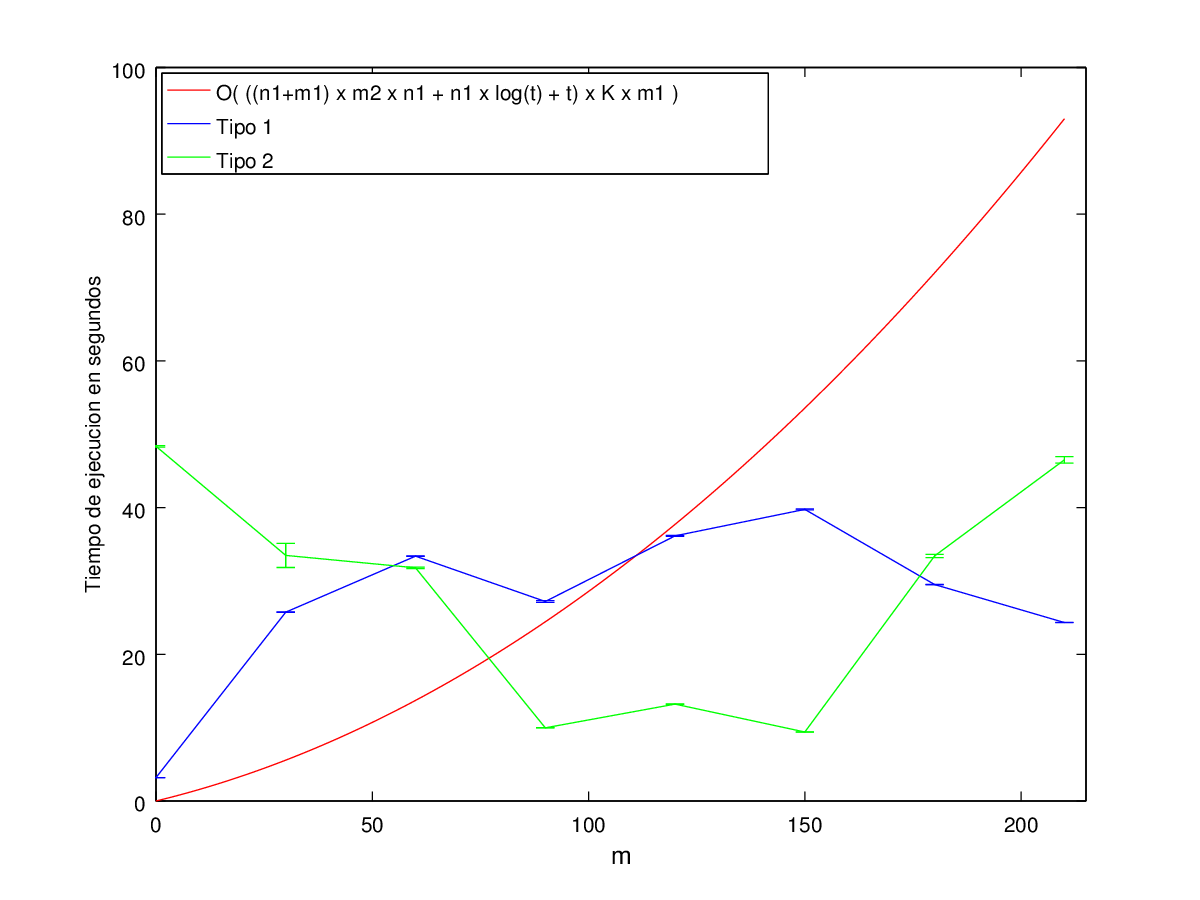
\includegraphics[height=10cm]{graficos/ejercicio6-exp1.png}
       \caption{Experimento 1}
	\end{figure}
\subsubsection*{Conclusiones}\;
        
        
        
\subsubsection*{Experimento 2}\;
\noindent Este experimento es similar al anterior, pero ahora se varía la cantidad de nodos. Para ello, para cada cantidad de nodos se definirá una función para determinar la cantidad de aristas que tendrá el grafo. \\
\noindent Se tuvieron en cuenta 4 funciones, con el fin de que el grafo obtenido no sea siempre uno especial y de esta forma poder analizar diferentes casos. 
        \begin{itemize}
        \item F1($n_1$) = $n_1$($n_1$-1))/2 = $m_1$ 
        \item F2($n_1$) = $n_1$-1 = $m_1$ 
        \item F3($n_1$) = 3$n_1$ = $m_1$ 
        \item F4($n_1$) = $n_1^{2}$/10 = $m_1$ 
		\end{itemize} 
Para generar los grafos con estas cantidades de aristas y nodos se utilizó el mismo generador que en el experimento anterior.
Este experimento se realizará de la misma manera utilizando primero la vecindad tipo 1 y luego la vecindad tipo 2.

\subsubsection*{Datos de entrada}\;
\noindent Los valores de $n_1$ tomados fueron desde $10$ hasta $30$ de $5$ en $5$. \\
       Los valores de $n_2$ y $m_2$ fueron $50$ y $30$ respectivamente. Estos valores fueron elegidos de forma arbitraria. Los valores de $cuantosVecinosMiro$, $tamanoMaximoListaTabu$ y $k$ fue $10$ para los $3$ parámetros.  Estos valores fueron elegidos de forma arbitraria. \\
        Para generar los grafos de forma aleatoria se utilizó el generador-grafo-rapido.cpp que se encuentra en la carpeta src y para correrlo se utilizó el exp2.sh que se encuentra en la carpeta exp/ejercicio6/exp2. \\
        Con el fin de acercarse a los valores reales y descartar posibles falsos resultados, se ejecuta la resolución del problema para cada una de los valores de $n_1$ cinco veces considerando luego el promedio entre los valores obtenidos pero graficando también el desvío estándar (la cantidad de repeticiones a realizar fue elegida arbitrariamente).\; 

\subsubsection*{Resultados}\;

    \begin{figure}[H]
      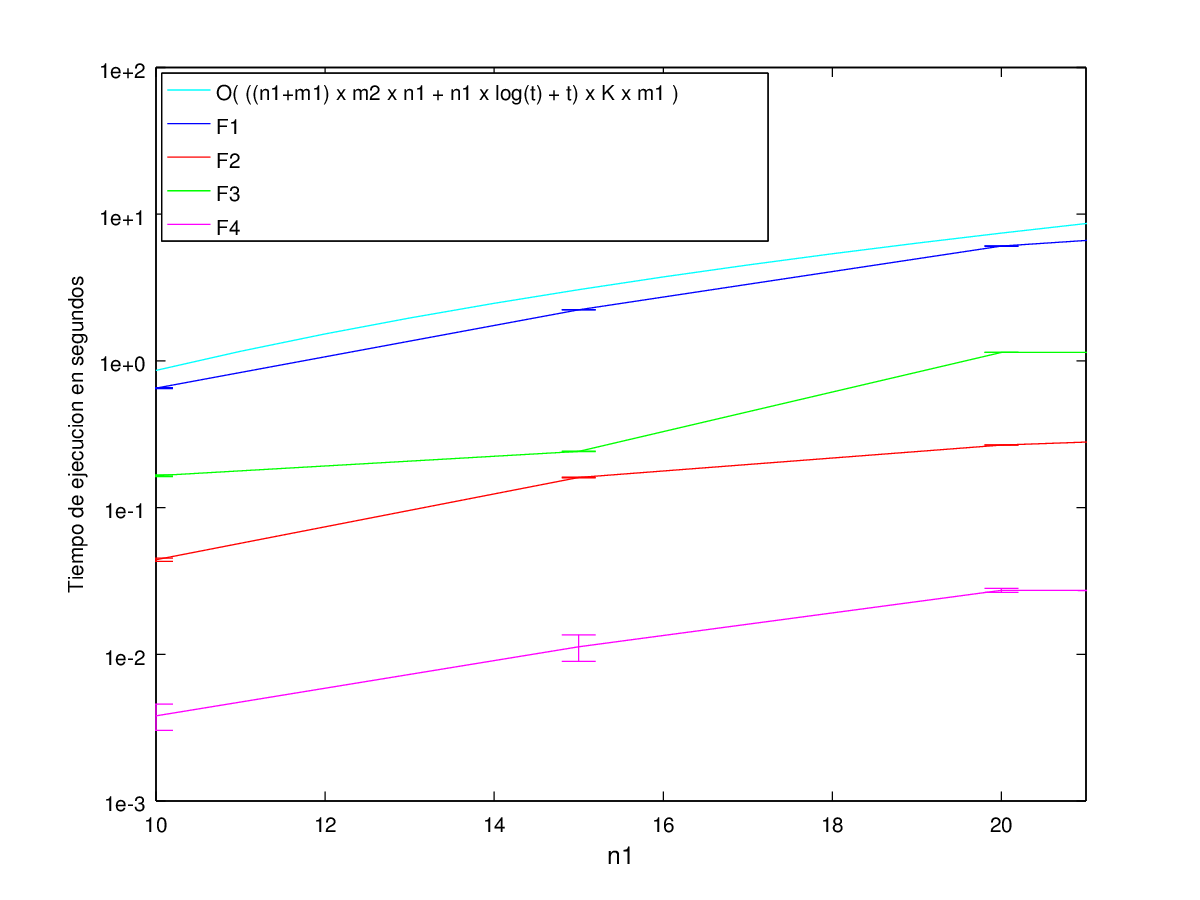
\includegraphics[height=10cm]{graficos/ejercicio6-exp2-tipo1.png}
       \caption{Experimento 2 - Vecindad tipo 1}
	\end{figure}

    \begin{figure}[H]
      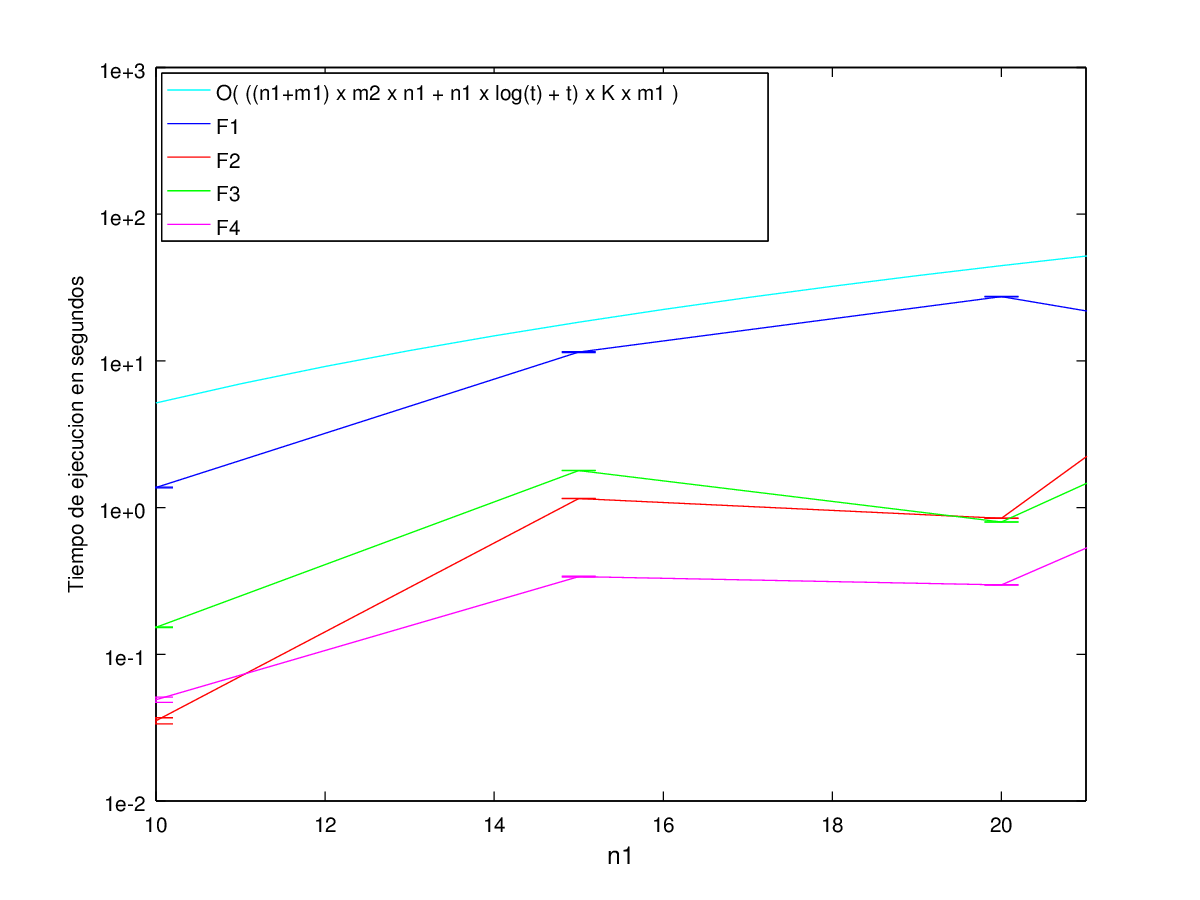
\includegraphics[height=10cm]{graficos/ejercicio6-exp2-tipo2.png}
       \caption{Experimento 2 - vecindad tipo 2}
	\end{figure}

\subsubsection*{Conclusiones}\;
Observamos que en todos los casos se respeta la complejidad propuesta(la curva de tiempo de computo se coloca por debajo de la de la cota de complejidad).\\
Se observa también comparando entre los 2 gráficos que el aplica vecindades del tipo 1 es considerablemente  mas rápido en todos los casos(en algunos mas que otros).Lo que nos lleva a concluir que el algoritmo de este tipo de vecindad se llega a ejecutar mas rápido, lo que no significa que sea el mejor pues para esto habría que analizar la calidad de las soluciones obtenidas(lo que haremos en un próximo experimento).\\ 
Adicionalmente se observa que el orden en que resultaron los tiempo de las distintas $F$ es el mismo en ambos grafos, lo que nos lleva a la conclusión de que los peores y mejores casos(al menos en cuanto a tiempo de computo) serán los mismos para ambos algoritmos.



\subsubsection*{Experimento 3}\; 
    El objetivo de este experimento fue extraer conclusiones acerca de la variación en el tiempo de cómputo requerido por el algoritmo para distintos valores de $m$ y $n$ variando los dos grafos al mismo tiempo pero siempre manteniendo $n_1$ igual a $n_2$ y $m_1$ igual a $m_2$. \\
Para generar los grafos con estas cantidades de aristas y nodos se utilizó el mismo generador que en el experimento anterior.
Este experimento se realizará utilizando primero la vecindad tipo 1 y luego la vecindad tipo 2.
        
\subsubsection*{Datos de entrada}\;
    \noindent Los valores de $n$ tomados fueron desde $10$ hasta $25$ de $5$ en $5$. Los valores de $cuantosVecinosMiro$, $tamanoMaximoListaTabu$ y $k$ fue $10$ para los $3$ parámetros. Estos valores fueron elegidos de forma arbitraria. \\
        Para generar los grafos de forma aleatoria se utilizó el generador-grafo-rapido.cpp que se encuentra en la carpeta src y para correrlo se utilizó el exp3.sh que se encuentra en la carpeta exp/ejercicio6/exp3. \\
        Con el fin de acercarse a los valores reales y descartar posibles falsos resultados, se ejecuta la resolución del problema para cada una de los valores de $n$ cinco veces considerando luego el promedio entre los valores obtenidos pero graficando también el desvío estándar (la cantidad de repeticiones a realizar fue elegida arbitrariamente).\; 

\subsubsection*{Resultados}\;

    \begin{figure}[H]
      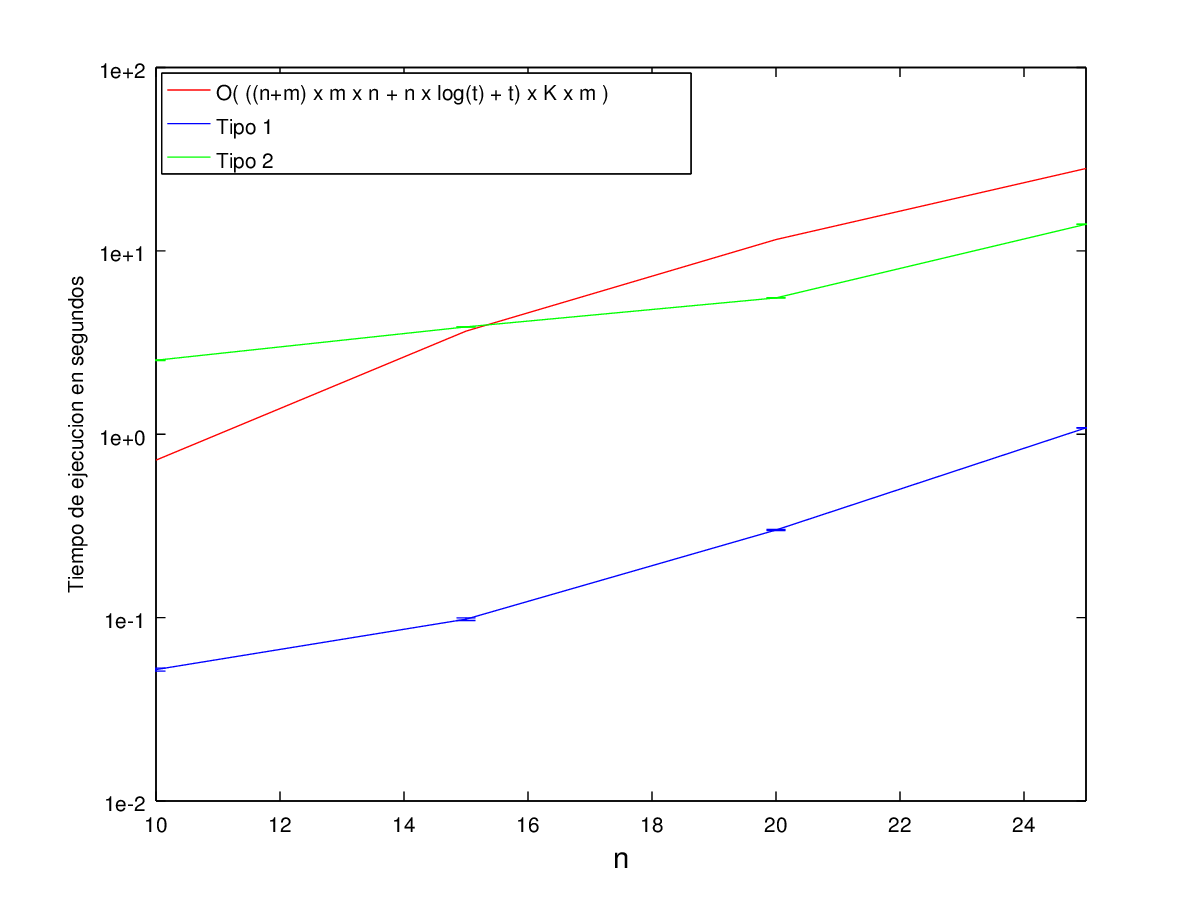
\includegraphics[height=10cm]{graficos/ejercicio6-exp3.png}
       \caption{Experimento 3}
	\end{figure}


\subsubsection*{Conclusiones}\;
Se observa en el gráfico, que ambos algoritmos parecen cumplir con la cota de complejidad asintótica propuesta, sin embargo, se puede ver también, como conjeturamos anteriormente, que el algoritmo de vecindades tipo 1 resulta ser mas eficiente que el de tipo 2, como ya dijimos esto no concluye que sea mejor pues sera necesario comparar primero la calidad de las soluciones, pero si podemos concluir que en cuanto al tiempo de ejecución es mejor el de vecindades tipo 1.


\subsubsection*{Experimento 4}\;
\noindent El objetivo de este experimento fue comparar los diferentes tipos de vecindades. Para ello se tomó en cuenta cuánto es el tiempo de cómputo y cuál es la cantidad de aristas que tiene el grafo solución para cada una de las vecindades. De esta forma, se logra analizar que vecindad es conveniente utilizar en determinados casos. Por ejemplo, en algunas ocasiones será beneficioso utilizar la vecindad que provea una respuesta en menor tiempo (aunque no sea la mejor) y en otras será ventajoso utilizar la vecindad que devuelva la solución más exacta posible, dándole más importancia a ésto que al tiempo que tarde en devolverla. \\
Para ello se utilizó el mismo generador que en el experimento 1.\\
Para realizar este experimento se ejecutaron las dos vecindades pasándoles por parámetro de entrada los mismos grafos, el mismo tamaño de la lista tabú, la misma cantidad de vecinos a tener en cuenta para cada iteración, y el mismo criterio de parada para poder realizar una comparación más exacta. 

\subsubsection*{Datos de entrada}\;
\noindent Los valores de $n_1$ tomados fueron desde $5$ hasta $20$ de $2$ en $2$. \\
       Los valores de $n_2$ y $m_2$ fueron $50$ y $200$ respectivamente. Los valores de $cuantosVecinosMiro$, $tamanoMaximoListaTabu$ y $k$ fue $10$ para los $3$ parámetros. Estos valores fueron elegidos de forma arbitraria. \\
        Para generar los grafos de forma aleatoria se utilizó el generador-grafo-rapido.cpp que se encuentra en la carpeta src y para correrlo se utilizó el exp4.sh que se encuentra en la carpeta exp/ejercicio6/exp4. \\
        Con el fin de acercarse a los valores reales y descartar posibles falsos resultados, se ejecuta la resolución del problema para cada una de los valores de $n_1$ cinco veces considerando luego el promedio entre los valores obtenidos pero graficando también el desvío estándar (la cantidad de repeticiones a realizar fue elegida arbitrariamente).\; 
\subsubsection*{Resultados}\;

    \begin{figure}[H]
      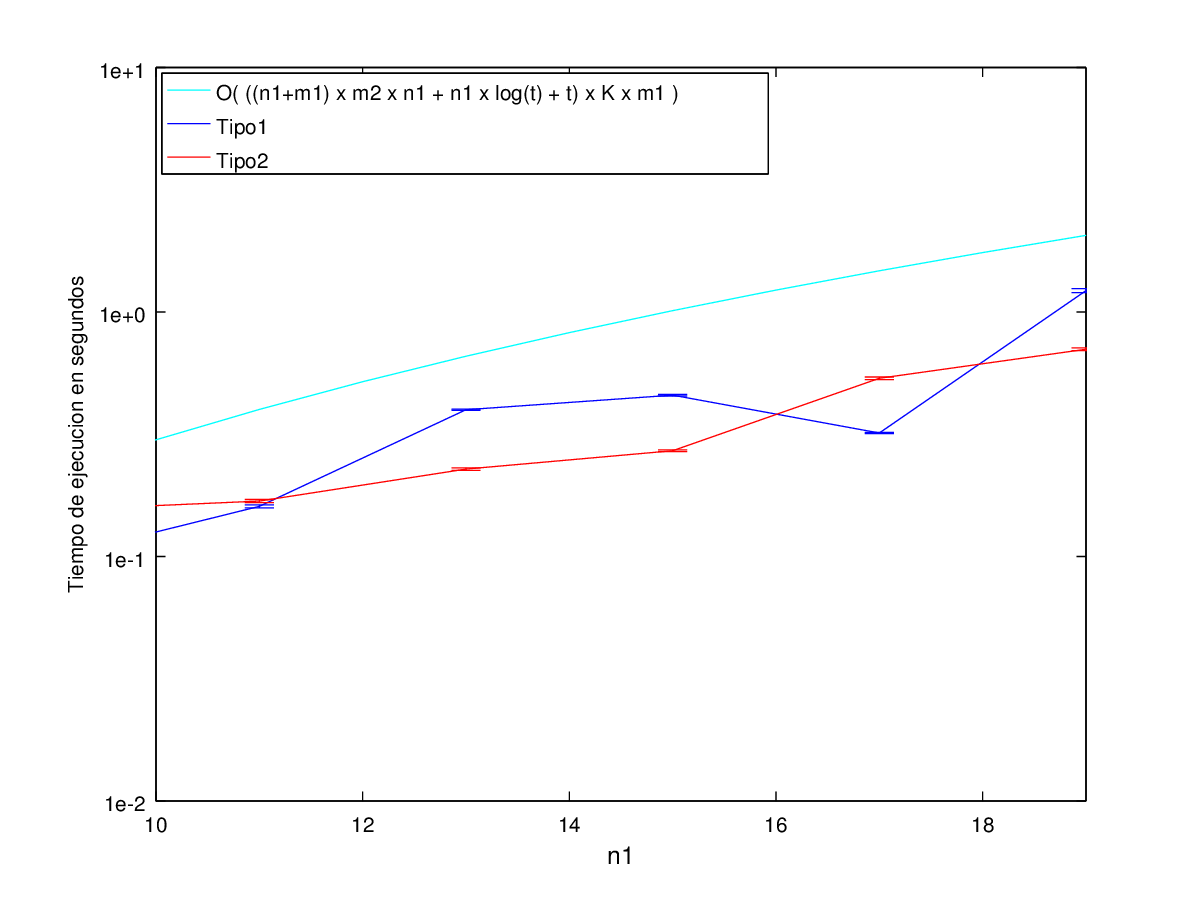
\includegraphics[height=10cm]{graficos/ejercicio6-exp4-tiempos.png}
       \caption{Experimento 4 - Comparando tiempos}
	\end{figure}

 \begin{figure}[H]
      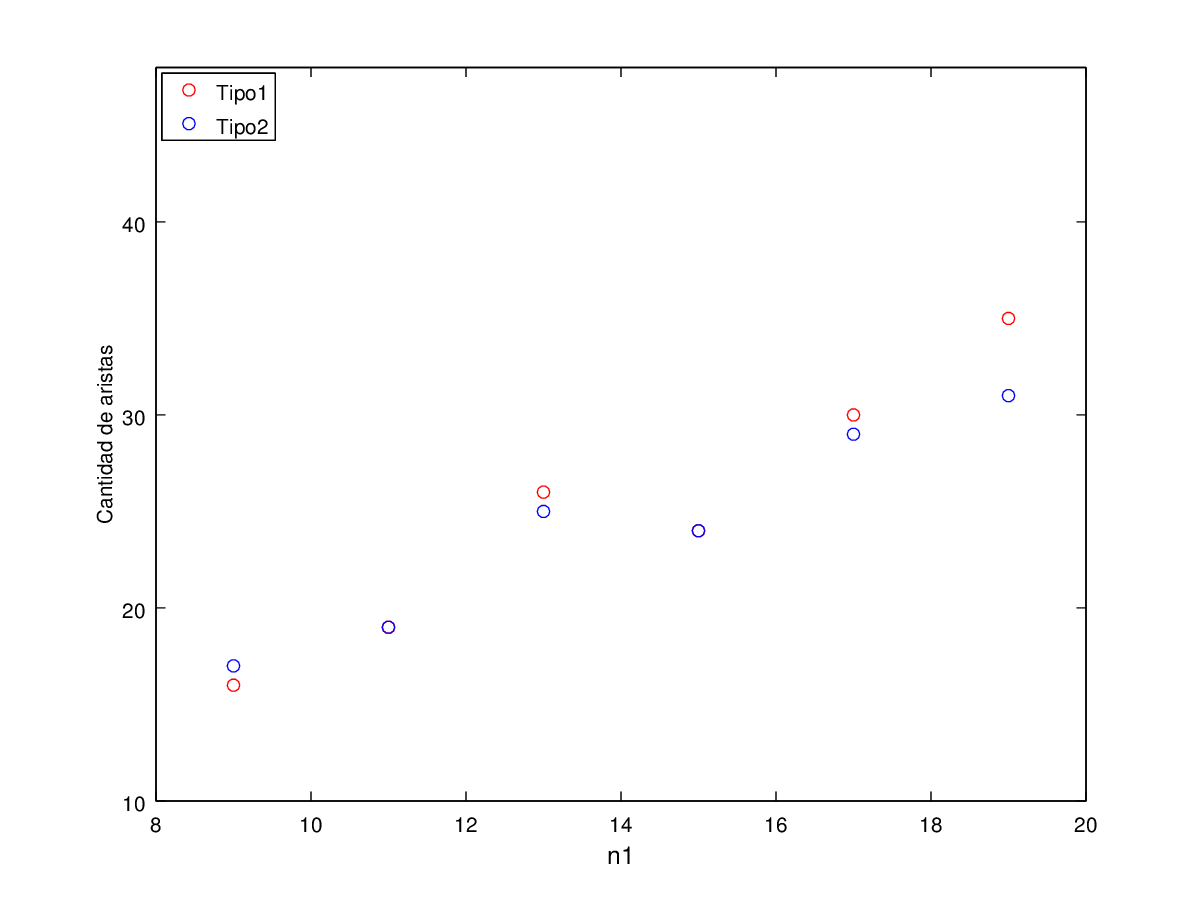
\includegraphics[height=10cm]{graficos/ejercicio6-exp4-aristas.png}
       \caption{Experimento 4 - Comparando cantidad de aristas}
	\end{figure}


\subsubsection*{Conclusiones}\;
En este Experimento el el gráfico de los tiempos, no se logra comprobar la conjetura de que el algoritmo con las vecindades tipo 1 es mas eficiente.\\
Se observa también del gráfico de los tiempos que ambos algoritmos se mantienen dentro del rango de complejidad esperada.\\
Finalmente, las conclusiones mas destacables de este experimento se pueden ver en el segundo gráfico, En este se ve como las soluciones brindadas por el algoritmo con las vecindades tipo 1 son superiores en todos los casos al de las vecindades tipo 2, en algunos casos se observa que la solución encontrada es considerablemente mejor(para la instancia de $n_1=20$), atribuimos a esta considerable diferencia el echo de que el algoritmo de tipo 1 resulto tardar mas para esta instancia que el de las vecindades tipo 2 a pesar de que experimentos pasados nos dieron el pie a conjeturar y concluir que las vecindades tipo 1 son también mas eficientes.\\
Concluimos entonces(con este experimento en conjunto con los anteriores):\\
El algoritmo de vecindades tipo 1 es considerablemente mejor en cuanto a la calidad de soluciones que provee.\\
El algoritmo de vecindades tipo 1 es mas eficiente excepto cuando encuentra una solución considerablemente mejor que la del algoritmo de vecindades tipo 2, en este caso podría resultar ligeramente mas lento.\\
Como conclusión general diremos que el algoritmo con las vecindades tipo 1 es mejor(para la gran mayoría de los casos).

\subsubsection*{Experimento 5}\;
\noindent En este experimento se buscará comparar cómo varía el tiempo de ejecución y la cantidad de aristas que tiene el grafo solución cuando se toman distintos tamaños máximos que puede tener la lista tabú. Para ello se dejarán constantes los grafos sobre los que se calcula el MCS, ambos generados de manera aleatoria, la cantidad de vecinos a tener en cuenta para cada iteración y el criterio de parada.\\
El generador utilizado será el mismo que en el experimento 1.\\
Se utilizará la vecindad que generó mejores resultados en el experimento anterior ya que el objetivo no es comparar entre vecindades si no comparar resultados cuando varía el tamaño de la lista tabú.

\subsubsection*{Datos de entrada}\;
\noindent Los valores de $tamanoMaximoListaTabu$ tomados fueron desde $5$ hasta $40$ de $5$ en $5$. \\
       Los valores de $n_1$ y $m_1$ fueron $50$ y $200$ respectivamente, al igual que $n_2$ y $m_2$ ($n_1 = n_2$ y $m_1 = m_2$). Los valores de $cuantosVecinosMiro$, y $k$ fue $10$ para los $2$ parámetros. Estos valores fueron elegidos de forma arbitraria. \\
        Para generar los grafos de forma aleatoria se utilizó el generador-grafo-rapido.cpp que se encuentra en la carpeta src y para correrlo se utilizó el exp5.sh que se encuentra en la carpeta exp/ejercicio6/exp5. \\
        Con el fin de acercarse a los valores reales y descartar posibles falsos resultados, se ejecuta la resolución del problema para cada una de los valores de $tamanoMaximoListaTabu$ cinco veces considerando luego el promedio entre los valores obtenidos pero graficando también el desvío estándar (la cantidad de repeticiones a realizar fue elegida arbitrariamente).\; 

\subsubsection*{Resultados}\;
    \begin{figure}[H]
      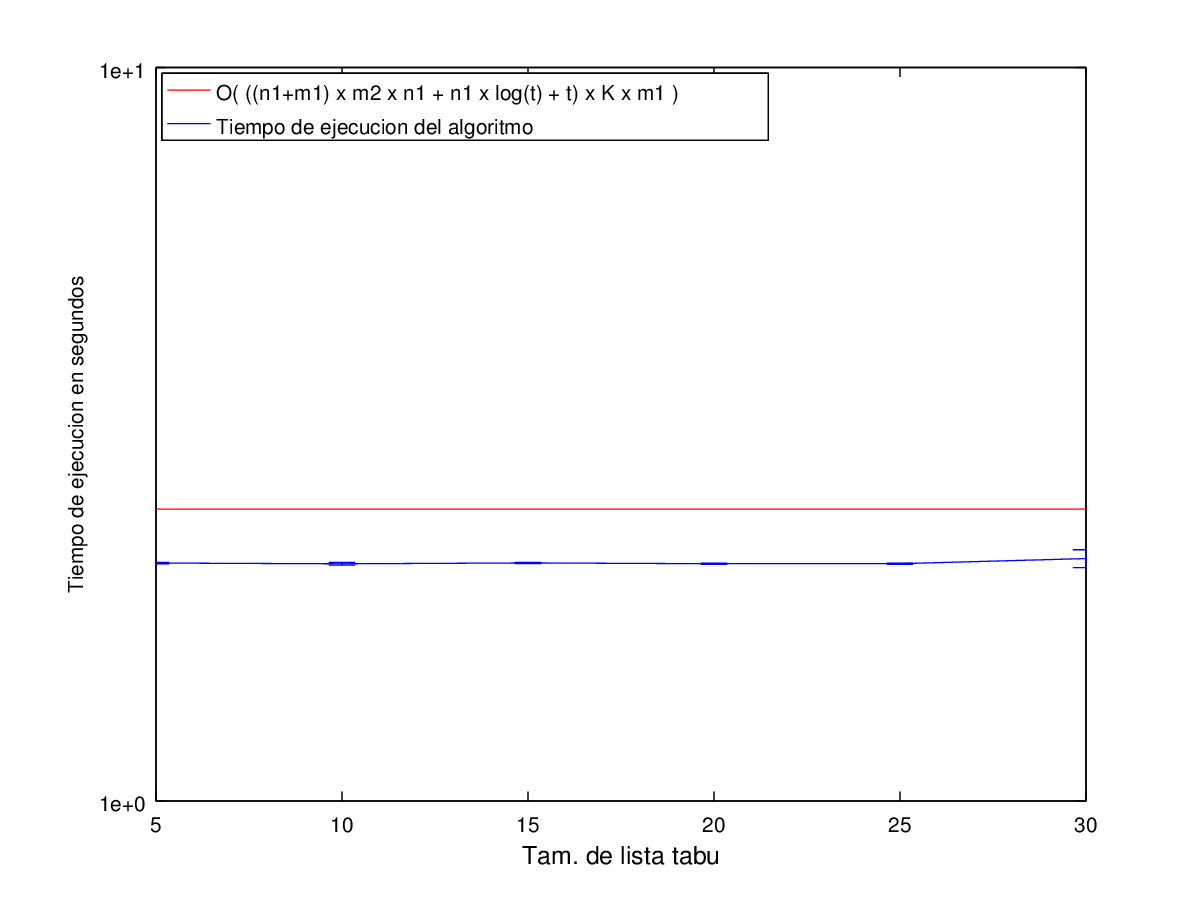
\includegraphics[height=10cm]{graficos/ejercicio6-exp5-tiempos.png}
       \caption{Experimento 5 - Comparando tiempos}
	\end{figure}

 \begin{figure}[H]
      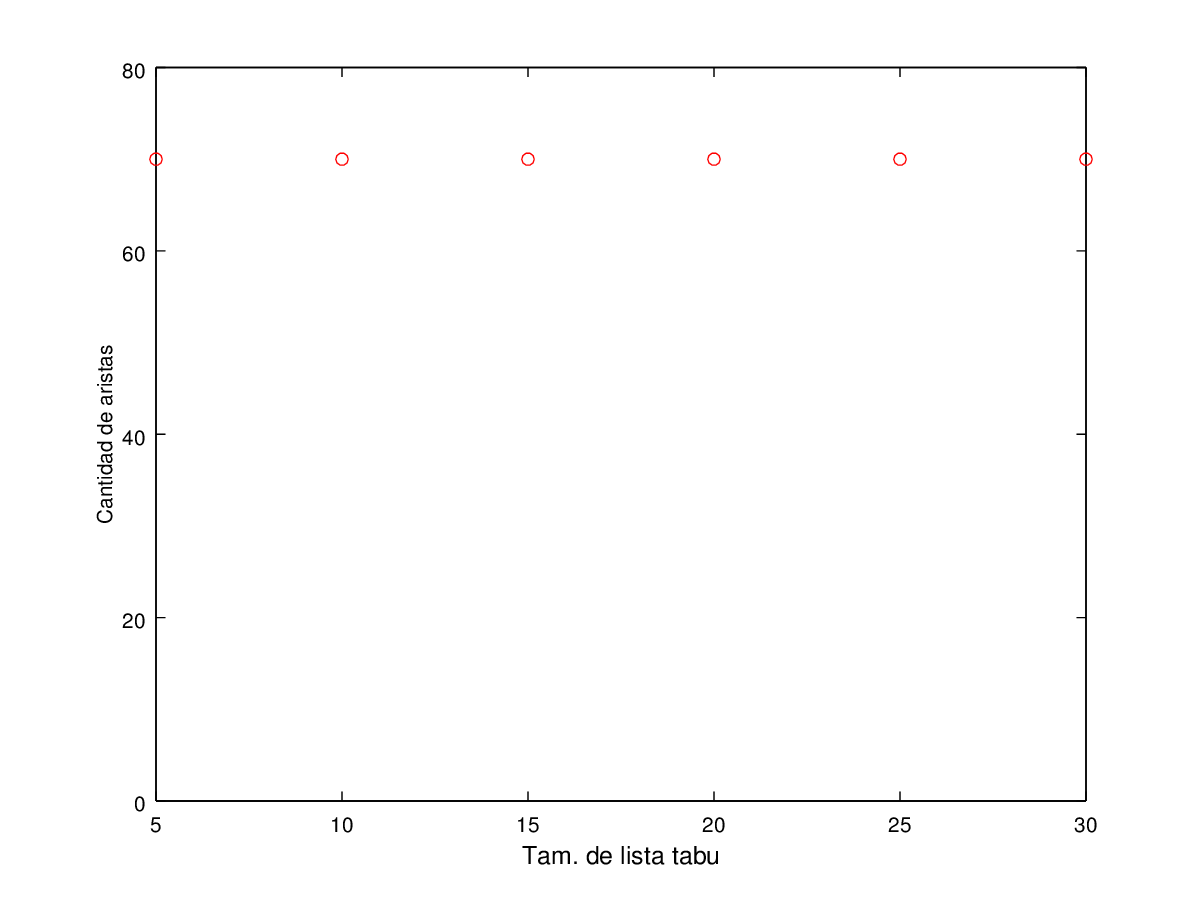
\includegraphics[height=10cm]{graficos/ejercicio6-exp5-aristas.png}
       \caption{Experimento 5 - Comparando cantidad de aristas}
	\end{figure}


\subsubsection*{Conclusiones}\;
Se observa que el tiempo de ejecución se mantiene constante a pesar del cambio en el tamaño de la lista tabú.Esto, conjeturamos, resulta así dado que:\\
-El tiempo de creación de la lista tabú, es irrelevante para el tiempo del problema, es decir el tiempo de crear la lista de t posiciones es despreciable en comparación al Tiempo que llevan las comparaciones de vecindades sucesivas.\\
-La lista tabú no parece llenarse siempre, es decir que por mas grande que se haga esta lista, solo se usa una parte reducida de esta, las búsquedas al ser logarítmicas en el tamaño de elementos tabú (multiplicado por $n_1$), puede despreciarse también en relación al resto del algoritmo ya que los ordenes de complejidad del resto de las operaciones son significativamente mas altos.\\ Incluso para n y m fijos,como es el caso hacer variar el t ligeramente, como esta echo, no parece contribuir significativamente, probablemente se deba a que el uso de la lista tabú es reducido.\\
Ademas cabe recalcar que la complejidad propuesta esta calculada en el caso del peor escenario posible, el cual es difícil de replicar y es poco probable que se re replique en un caso aleatorio(esto esta explicado en el desarrollo de complejidad).\\
Concluimos entonces que la gran mayoría de los casos el tamaño de la lista tabú no es un factor influyente en la cantidad de aristas ni en el tiempo de computo(a pesar de aparecer en la complejidad del peor caso, este peor caso es un caso excepcional y poco común).
 
\subsubsection*{Experimento 6}\;
\noindent En este experimento se buscará comparar cómo varía el tiempo de ejecución y la cantidad de aristas que tiene el grafo solución cuando se toman distintas cantidades de vecinos a tomar en cuenta para cada iteración. Para ello se dejarán constantes los grafos sobre los que se calcula el MCS, ambos generados de manera aleatoria, el tamaño máximo que puede tomar la lista tabú y el criterio de parada.\\
El generador utilizado será el mismo que en el experimento 1.\\
Se utilizará la vecindad que generó mejores resultados en los primeros experimentos ya que el objetivo no es comparar entre vecindades si no comparar resultados cuando varían las cantidades de vecinos a tomar en cuenta para cada iteración.

\subsubsection*{Datos de entrada}\;
\noindent Los valores de $cuantosVecinosMiro$ tomados fueron desde $5$ hasta $30$ de $5$ en $5$. \\
       Los valores de $n_1$ y $m_1$ fueron $50$ y $200$ respectivamente, al igual que $n_2$ y $m_2$ ($n_1 = n_2$ y $m_1 = m_2$). El valor de $tamanoMaximoListaTabu$ fue $20$ y $k$ fue $10$. Estos valores fueron elegidos de forma arbitraria. \\
        Para generar los grafos de forma aleatoria se utilizó el generador-grafo-rapido.cpp que se encuentra en la carpeta src y para correrlo se utilizó el exp6.sh que se encuentra en la carpeta exp/ejercicio6/exp6. \\
        Con el fin de acercarse a los valores reales y descartar posibles falsos resultados, se ejecuta la resolución del problema para cada una de los valores de $cuantosVecinosMiro$ cinco veces considerando luego el promedio entre los valores obtenidos pero graficando también el desvío estándar (la cantidad de repeticiones a realizar fue elegida arbitrariamente).\; 
        
\subsubsection*{Resultados}\;
    \begin{figure}[H]
      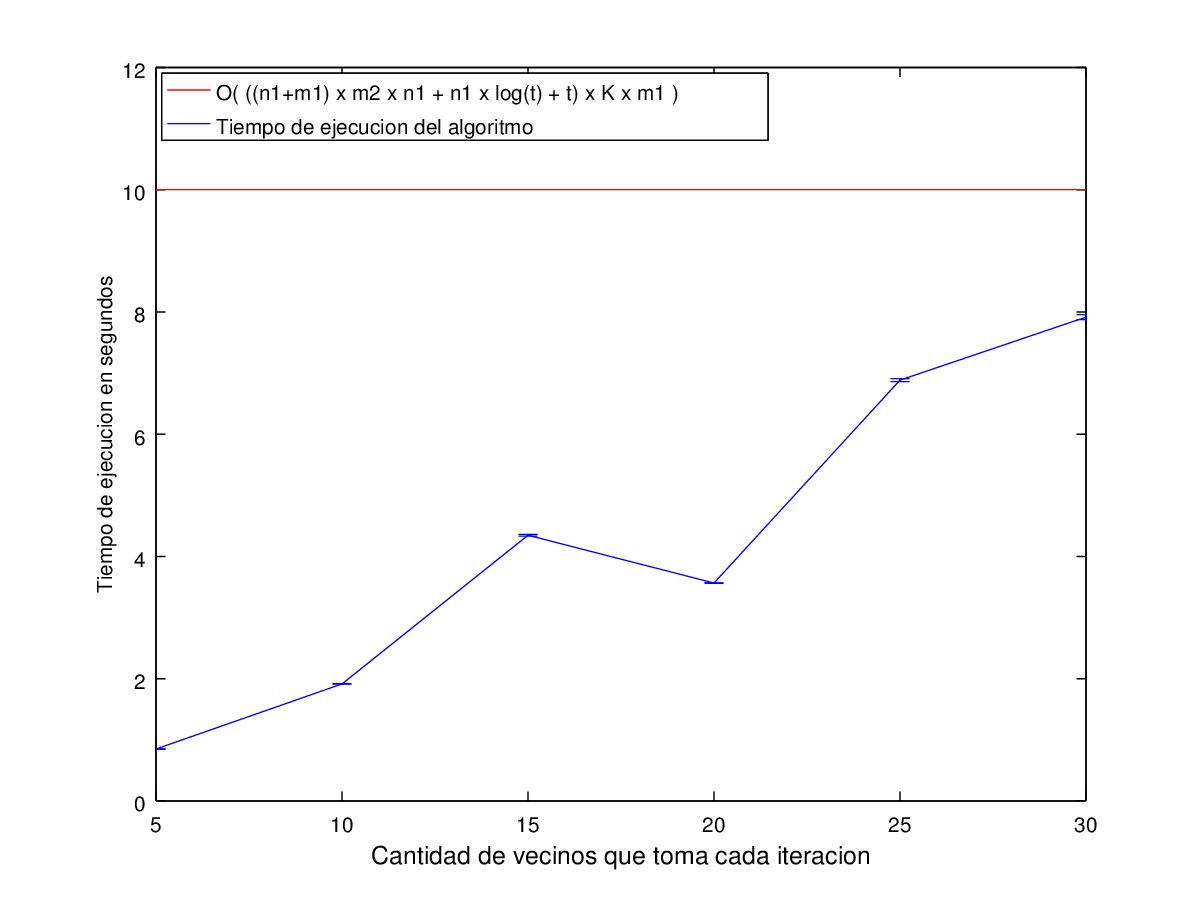
\includegraphics[height=10cm]{graficos/ejercicio6-exp6-tiempos.png}
       \caption{Experimento 6 - Comparando tiempos}
	\end{figure}

 \begin{figure}[H]
      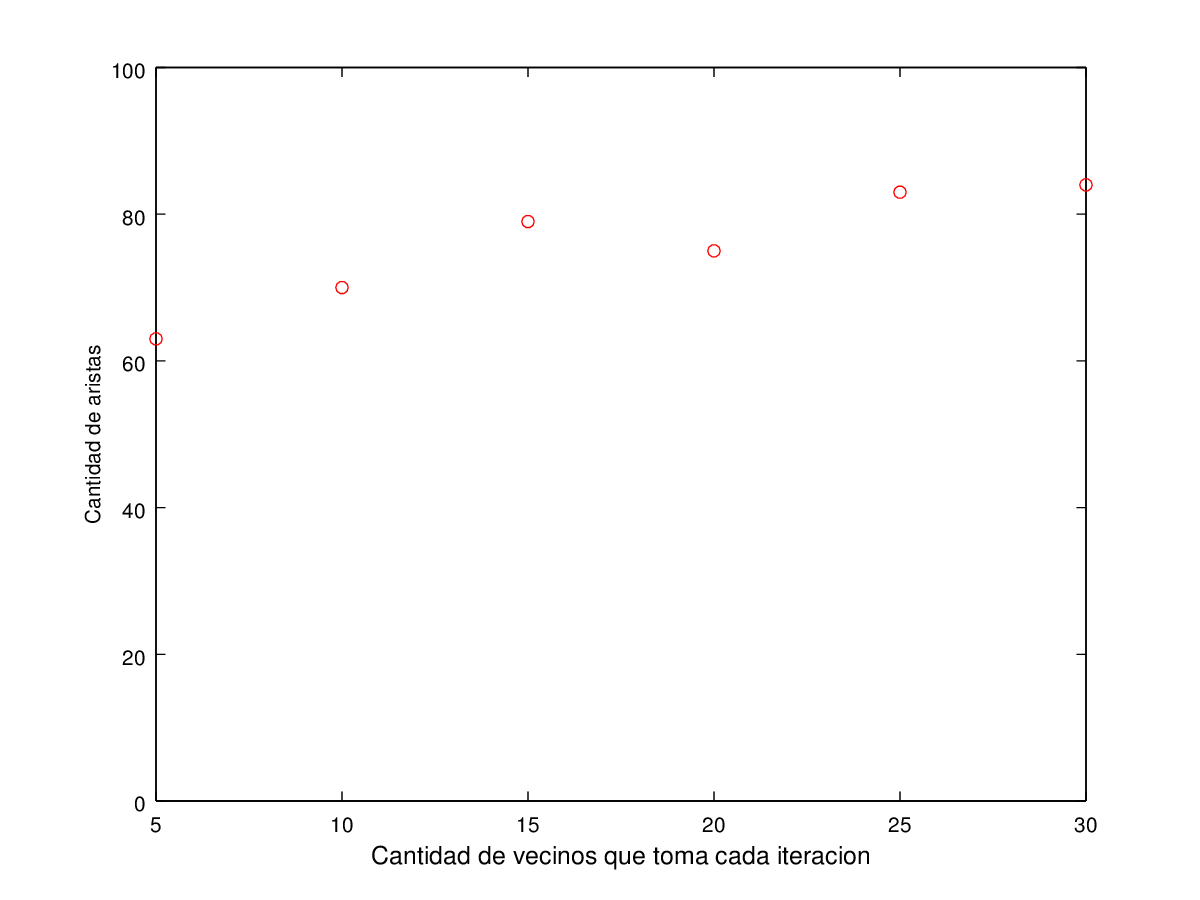
\includegraphics[height=10cm]{graficos/ejercicio6-exp6-aristas.png}
       \caption{Experimento 6 - Comparando cantidad de aristas}
	\end{figure}


\subsubsection*{Conclusiones}\;
En el primer gráfico (el de tiempos) se observa como influye de manera cuasi-linear la cantidad de vecinos a tomar en cada iteración hasta llegar al limite de $n_1$ vecinos , que es el tamaño de toda la vecindad(es por esto que la linea de cota es una constante) esta constante da la cota en caso que la cantidad de vecinos a tomar sea $n_1$ osea toda la vecindad, como el resto de los parámetros se mantienen constantes la cota sera constante.\\
En el segundo gráfico apreciamos que la diferencia entre cantidad de vecinos a tomar variara la cantidad de aristas en la solución(hay un incremento de aproximadamente un 25\%, solo variando la cantidad de vecinos a tomar).\\
Concluimos entonces que reducir el numero de vecinos a tener en cuenta puede ser útil para reducir el tiempo de computo (se reduce linealmente el tiempo) especialmente en los casos que $n_1$ es relativamente grande(recordamos que $n_1$, hace referencia a la cantidad de nodos del grafo mas chico),En cambio si alguno de los 2 grafos es relativamente chico sera aconsejable que la cantidad de vecinos que se toman en cuenta sea alta(cuanto mas cercano a $n_1$ mejor) pues en este caso no afectara mucho al tiempo de computo y puede mejorar la solución considerablemente.\\
Por otra parte incluso en grafos de gran cantidad de nodos($n_1$ grande) puede ser positivo establecer una cantidad de vecinos a considerar alta ya que es altamente probable que mejore la solución considerablemente, aunque en contraposición si se notara un incremento en el tiempo de computo.


\subsubsection*{Experimento 7}\;
\noindent En este experimento se buscará comparar cómo varía el tiempo de ejecución cuando varía la cantidad de iteraciones que deben pasar sin obtener una solución mejor a la que se tiene hasta el momento y termine de ejecutar el algoritmo(el criterio de parada,el  K). Para ello se dejan constantes los grafos sobre los que se calcula el MCS, ambos generados de manera aleatoria, el tamaño máximo que puede tomar la lista tabú y la cantidad de vecinos a tomar en cuenta para cada iteración.\\
El generador utilizado será el mismo que en el experimento 1.\\
Se utilizará la vecindad que generó mejores resultados en los primeros experimentos ya que el objetivo no es comparar entre vecindades si no comparar resultados cuando varía la cantidad de iteraciones que deben pasar sin obtener una solución mejor a la que se tiene hasta el momento y termine de ejecutar el algoritmo.

\subsubsection*{Datos de entrada}\;
\noindent Los valores de $k$ tomados fueron desde $5$ hasta $25$ de $5$ en $5$. \\
       El valor de $n_1$ fue $1000$ y el de $n_2$ fue $150$. El de $m_1$ fue $200$ al igual que $m_2$.  Los valores de $cuantosVecinosMiro$ y $tamanoMaximoListaTabu$ fue $20$ para los $2$ parámetros. Estos valores fueron elegidos de forma arbitraria. \\
        Para generar los grafos de forma aleatoria se utilizó el generador-grafo-rapido.cpp que se encuentra en la carpeta src y para correrlo se utilizó el exp7.sh que se encuentra en la carpeta exp/ejercicio6/exp7. \\
        Con el fin de acercarse a los valores reales y descartar posibles falsos resultados, se ejecuta la resolución del problema para cada una de los valores de $k$ cinco veces considerando luego el promedio entre los valores obtenidos pero graficando también el desvío estándar (la cantidad de repeticiones a realizar fue elegida arbitrariamente).\;
\subsubsection*{Resultados}\;
    \begin{figure}[H]
      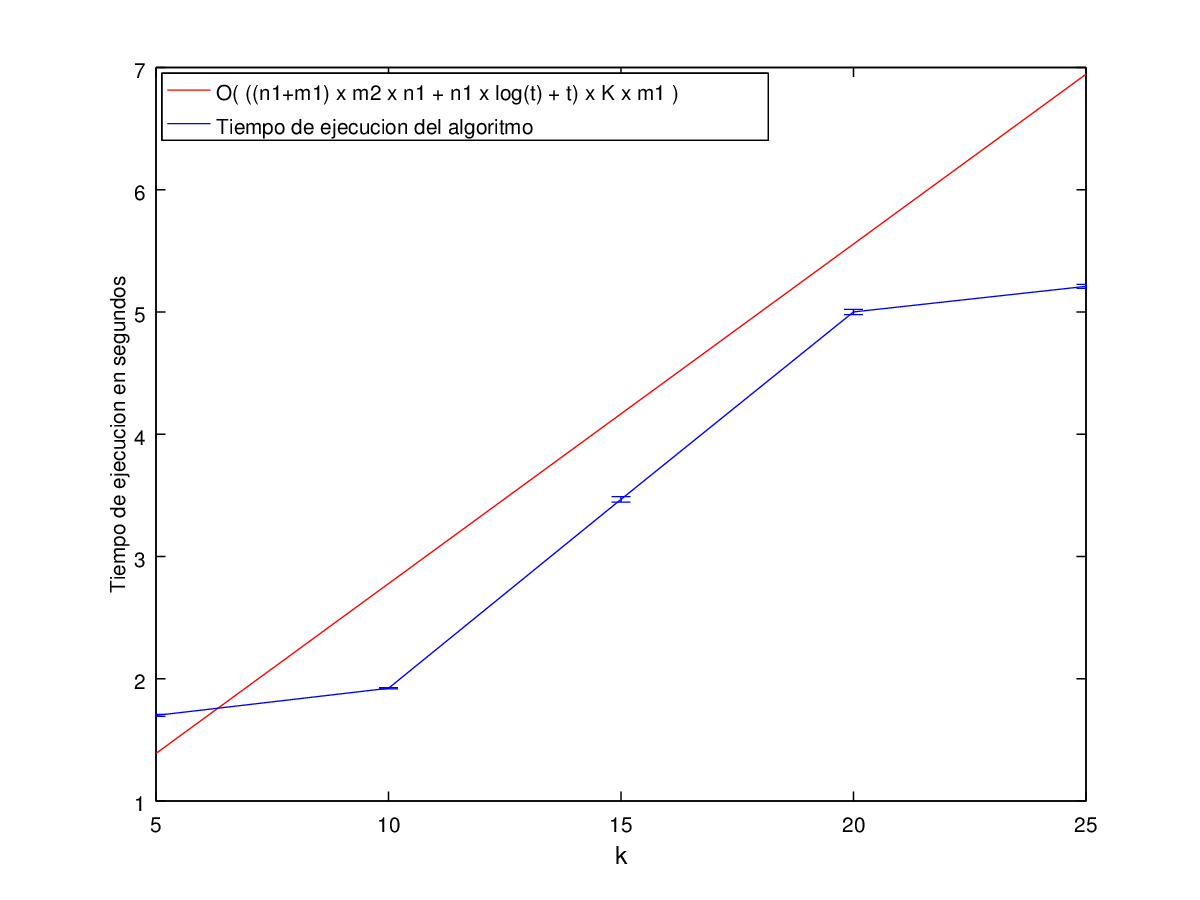
\includegraphics[height=10cm]{graficos/ejercicio6-exp7-tiempos.png}
       \caption{Experimento 7 - Comparando tiempos}
	\end{figure}



\subsubsection*{Conclusiones}\;
Se observa como era esperado el comportamiento aproximadamente lineal en $k$(el limite, criterio de parada o cantidad de veces que continua el algoritmo sin encontrar nada mejor).\\
Concluimos de este experimento que el aumento del criterio de parada aumenta el tiempo de computo linealmente aunque aumentarlo puede eventualmente llevar a una mejor solución.


\clearpage
  \section{Ejercicio 7}

\subsection{Introducción}
En este ejercicio se busca comparar las diferentes heurísticas y metaheuríticas halladas para resolver el problema de encontrar el máximo subgrafo común entre dos grafos. Para ello no sólo se compararán los tiempos de ejecución sino que también se tomará en cuenta cuántas aristas tiene el grafo solución para cada uno de los algoritmos. Este resultado se lo comparará, en los casos en los que sea posible, con los resultados obtenidos en el algoritmo exacto, es decir, se observará qué tan lejos de la solución óptima se encuentra el resultado obtenido con los algoritmos heurísticos. Esto no es posible de hacer en cualquier caso ya que, como sabemos, el algoritmo exacto resuelve un problema de tipo NP-completo y si se corre el algoritmo con un grafo de tamaño muy grande tardaría muchísimo tiempo en devolver un resultado. Para poder comparar con el resultado correcto se utilizarán grafos especiales ($C_n$, bipartito, bipartito completo, $K_n$, árboles (que son una clase particular de bipartitos), estrellas (también bipartitos, son $K_{1n}$), cografos, etc) ya que al utilizarlos se puede calcular de forma manual cuántas aristas en común tienen los grafos o se puede correr el algoritmo y que sea exacto sin que tarde demasiado tiempo (como es el caso de los cografos y completos).

\subsection{Experimentación}
    
\subsubsection*{Experimento 1}\;
 El objetivo de este experimento fue extraer conclusiones acerca de la variación en el tiempo de cómputo requerido por cada una de las heurísticas cuando se varían los valores de $n_1$ dejando $m_1$ $=$ 3$n_1$. \\
 Esperaremos que el experimento determine que la heurística mas rápida es la golosa, seguida de de búsqueda local y por ultimo la Tabú, nuestro fundamento para esto esta en que cada una es una ampliación de la anterior, es decir la búsqueda local, primero usa la heurística golosa y la Tabú usa reiteradamente el proceso(muy similar a) búsqueda Local.\\

Para ello se utilizará un generador de grafos que funciona de la siguiente manera: dada una cantidad de nodos y aristas, en cada paso crea una nueva arista con extremos válidos (es decir, entre 0 y la cantidad de nodos - 1) y que no esté repetida (que no haya sido creada todavía).\\
Para las heurísticas que cuentan con más de una versión (aquellas que tienen diferentes criterios para determinar lo que es una vecindad, o como la heurística de búsqueda tabú que se puede variar el tamaño de la misma, los vecinos a tener en cuenta en cada iteración y el criterio de parada) se tomó la combinación de variantes que dio mejores resultados en los experimentos realizados para el análisis particular de cada una de ellas.\\
Se sabe que para comparar bien las heurísticas es necesario variar todas las combinaciones de parámetros pero a fines de este TP, y para mantener acotado el alcance del mismo, dada la cantidad de experimentos que hemos hecho, vamos a experimentar con grafos con la misma cantidad de vértices y de aristas.

\subsubsection*{Datos de entrada}\;
\noindent Los valores de $n_1$ tomados fueron desde $10$ hasta $70$ de $5$ en $5$. \\
       Los valores de $n_2$ y $m_2$ fueron $50$ y $500$ respectivamente. Los valores de $tamanoMaximoListaTabu$ y $k$ fue $10$. El valor de $cuantosVecinosMiro$, tanto para la heurística de búsqueda local como para tabú, fue $20$. Estos valores fueron elegidos de forma arbitraria. \\
        Para generar los grafos de forma aleatoria se utilizó el generador-grafo-rapido.cpp que se encuentra en la carpeta src y para correrlo se utilizó el exp1.sh que se encuentra en la carpeta exp/ejercicio7/exp1. \\
        Con el fin de acercarse a los valores reales y descartar posibles falsos resultados, se ejecuta la resolución del problema para cada una de los valores de $n_1$ cinco veces considerando luego el promedio entre los valores obtenidos pero graficando también el desvío estándar (la cantidad de repeticiones a realizar fue elegida arbitrariamente).\; 

\subsubsection*{Resultados}\;
    \begin{figure}[H]
      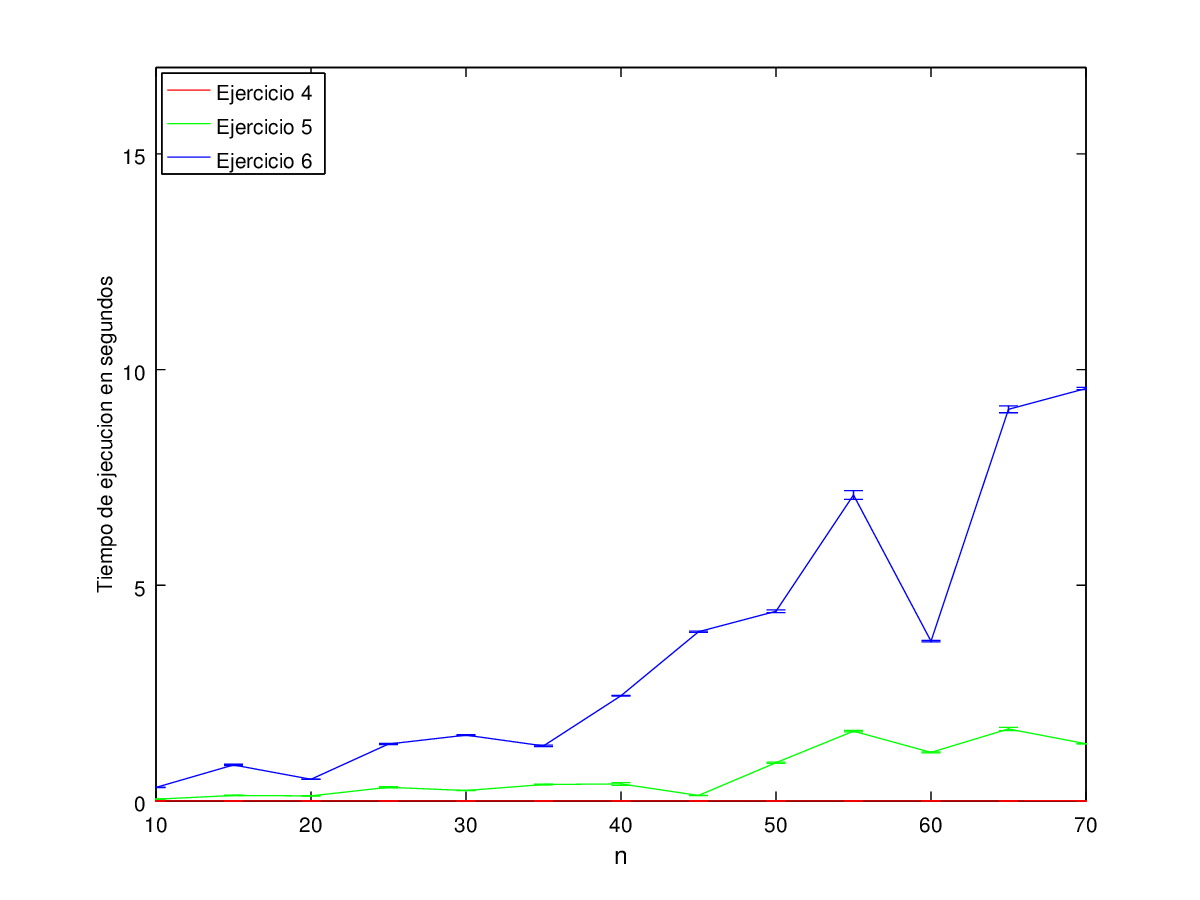
\includegraphics[height=10cm]{graficos/ejercicio7-exp1-tiempos.png}
       \caption{Experimento 1 - Comparando tiempos}
	\end{figure}

\subsubsection*{Conclusiones}\;
Como era esperado, El experimento muestra en el gráfico, como el en cuanto a tiempos de computo, lo mas rápido el la heurística golosa, en segundo lugar la búsqueda local y por ultimo la meta-heurística Tabú.Esto era de esperarse dado que cada una esta comprendida dentro de la anterior como ya explicamos. Por lo que es esperable que los tiempos de computo vayan en incremento, a su vez también sera esperable que la calidad de las soluciones también sea en aumento, ya que si una solución la encontró la heurística golosa, seguro también la encontró la local y también seguro la búsqueda Tabú.\\
Por ultimo notamos la magnitud de la diferencia en el tiempo tardado, la diferencia entre la golosa y la local, es significativa pero tal vez mas aceptable que la Tabu, que su tiempo tiene picos mucho mas altos.\\
Esto nos hace concluir que incluso que la tabú resulte mejor en calidad de solución, puede que para ciertos problemas en donde la performance sea un factor decisivo se prefiera usar la heurística de búsqueda local e incluso la golosa.

\subsubsection*{Experimento 2}\;
 El objetivo de este experimento fue extraer conclusiones acerca de la variación en la cantidad de aristas que contiene el subgrafo respuesta para cada una de las heurísticas cuando se varían los valores de $m$ y $n$ modificando los dos grafos al mismo tiempo pero siempre manteniendo $n_1$ igual a $n_2$ y $m_1$ igual a $m_2$. \\
Para ello, para cada cantidad de nodos se definirá una función para determinar la cantidad de aristas que tendrá el grafo. Estas funciones son las mismas que en el experimento anterior.\\
Al igual que antes, para las heurísticas que cuentan con mas de una versión, se tomó la combinación de variantes que dió mejores resultados en los experimentos realizados para el análisis particular de cada una de ellas.\\
Para generar los grafos con estas cantidades de aristas y nodos se utilizó el mismo generador que en el experimento anterior.\\

\subsubsection*{Datos de entrada}\;

Este experimento tiene los mismos datos de entrada que el anterior y se genera de la misma manera. Al generar uno automáticamente se crea el otro.

\subsubsection*{Resultados}\;
  \begin{figure}[H]
      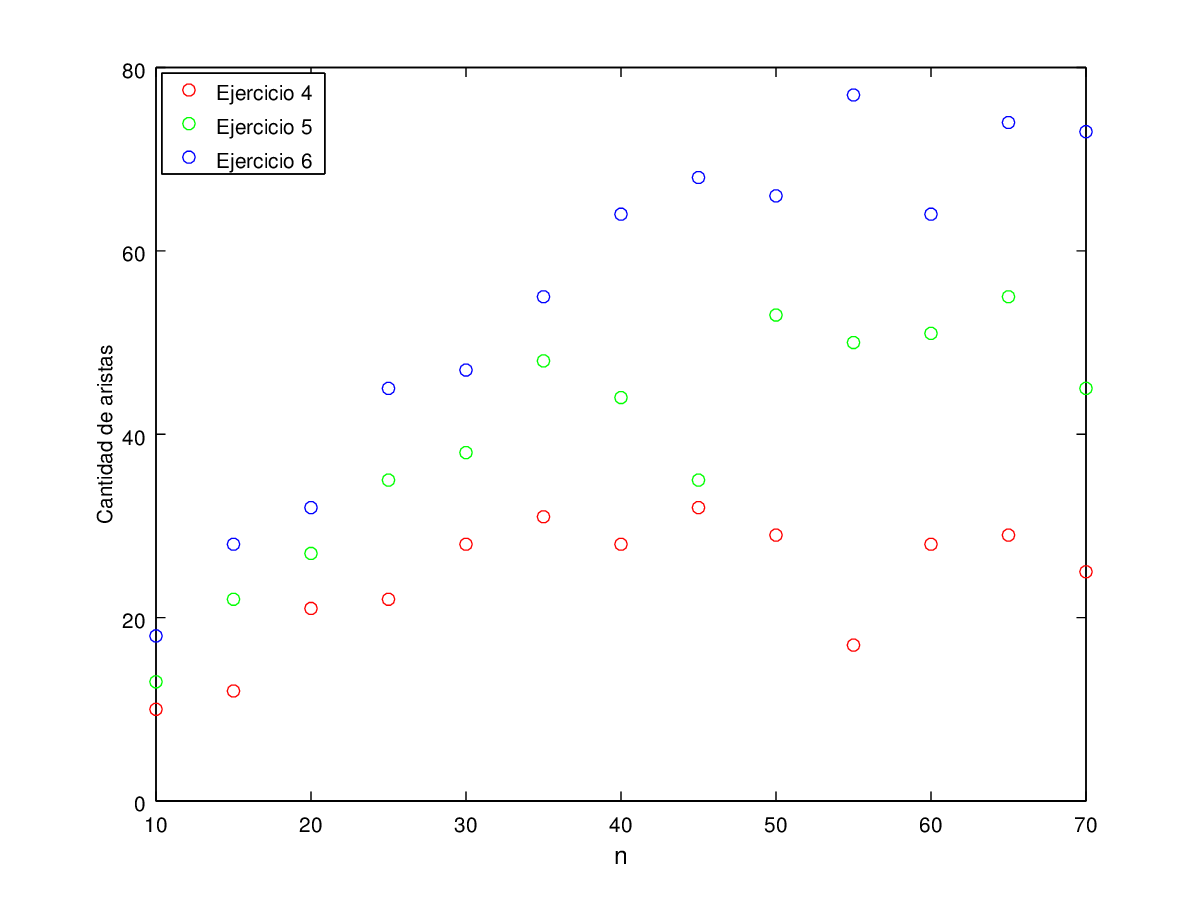
\includegraphics[height=10cm]{graficos/ejercicio7-exp2-aristas.png}
       \caption{Experimento 2 - Comparando aristas}
	\end{figure}
    
\subsubsection*{Conclusiones}\;

Como se puede observar, las heurísticas que requieren mayor tiempo de ejecución son las que dan mejores resultados por lo que no se puede comparar de manera directa entre todas las heurísticas(no se puede determinar una que sea absolutamente mejor). Dependiendo de cuál es la característica que se desea priorizar se elegirá una heurística. Por ejemplo, supongamos el caso de una empresa encargada de repartir correo a la que le llegan las cartas con las direcciones a donde deben ser enviadas muy poco tiempo antes de que los carteros deban salir a repartirlas. Sea el algoritmo que determina cual es el camino mas eficiente para recorrer las calles de la ciudad de tipo NP-completo para el que se desarrollan heurísticas para aproximar en menor tiempo el camino buscado. En este caso convendrá utilizar las heurísticas que requieran poco tiempo de ejecución sin importar si la solución no fue la mejor que se pudo obtener ya que los carteros deben salir a horario. \\
En cambio, el caso de una empresa que necesita cada 5 años éste cálculo convendrá utilizar la heurística más exacta posible ya que no importa mucho cuánto tiempo tarde en ejecutarse.\\ 
Para poder analizar un caso genérico debemos dejar constante una de las dos variables que tenemos (tiempo y correctitud). Como no se tiene control sobre la solución que brinda cada heurística lo que se puede hacer es dejar el tiempo fijo y hacer que todas terminen una vez pasado ese tiempo. Luego se comparará cuál es el resultado que cada algoritmo calculó hasta el momento y ahí sí podemos decir que para cierta instancia una se comporta mejor que la otra.

\subsubsection*{Experimento 3}\;
En este experimento compararemos los resultados que se obtienen de cada heurística cuando se ejecutan todas una misma cantidad de tiempo.\\
Para ello, para cada cantidad de nodos se definirá una función para determinar la cantidad de aristas.\\
Al igual que antes para las heurísticas que cuentan con más de una versión se tomó la combinación de variantes que dio mejores resultados en los experimentos realizados para el análisis particular de cada una de ellas.\\


\subsubsection*{Datos de entrada}\;
\noindent Los valores de $n_1$ tomados fueron desde $10$ hasta $70$ de $5$ en $5$. \\
       Los valores de $n_2$ y $m_2$ fueron $50$ y $200$ respectivamente. Los valores de $tamanoMaximoListaTabu$ y $k$ fue $10$. El valor de $cuantosVecinosMiro$, tanto para la heurística de búsqueda local como para tabú, fue $20$. Estos valores fueron elegidos de forma arbitraria. \\
        Para generar los grafos de forma aleatoria se utilizó el generador-grafo-rapido.cpp que se encuentra en la carpeta src y para correrlo se utilizó el exp3.sh que se encuentra en la carpeta exp/ejercicio7/exp3. \\
        Con el fin de acercarse a los valores reales y descartar posibles falsos resultados, se ejecuta la resolución del problema para cada una de los valores de $n_1$ cinco veces considerando luego el promedio entre los valores obtenidos pero graficando también el desvío estándar (la cantidad de repeticiones a realizar fue elegida arbitrariamente).\; 
\subsubsection*{Resultados}\;
  \begin{figure}[H]
      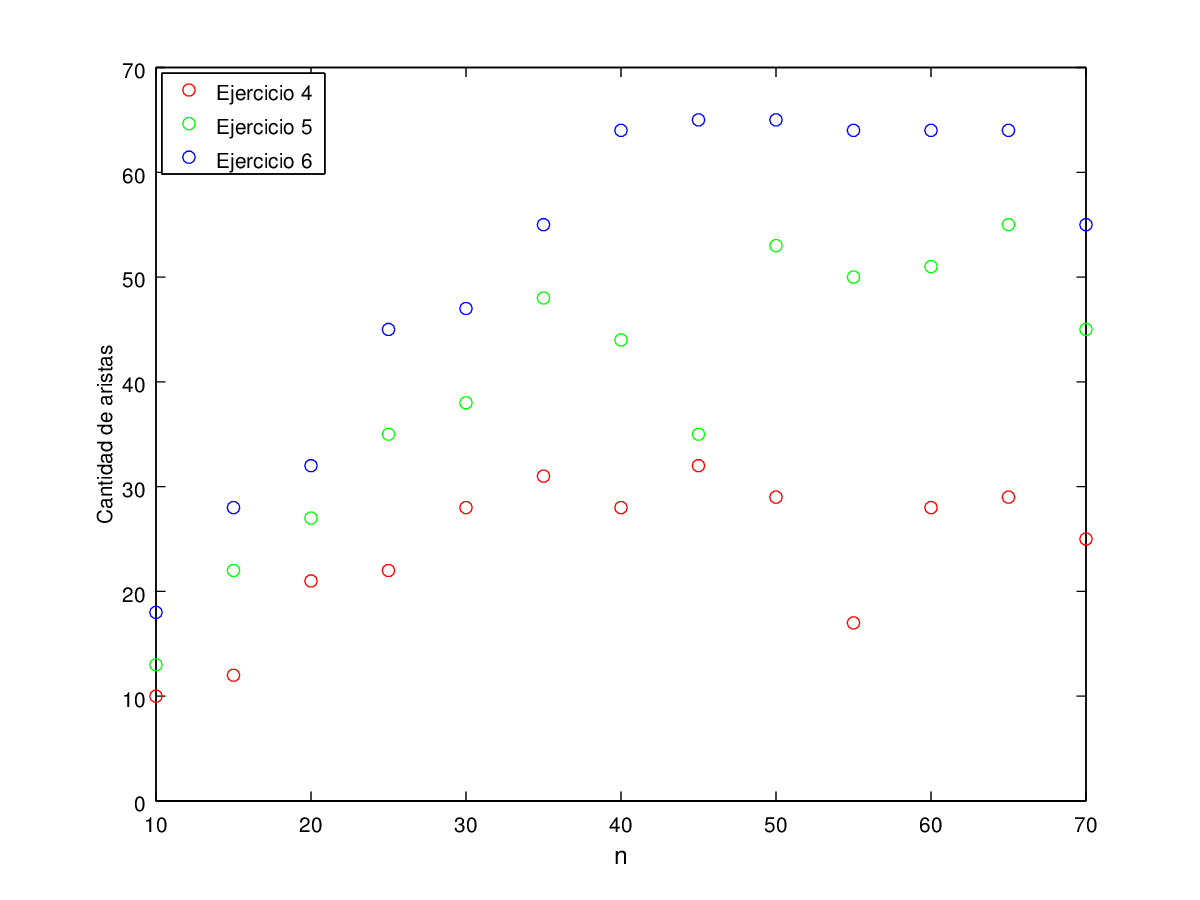
\includegraphics[height=10cm]{graficos/ejercicio7-exp3-aristas.png}
       \caption{Experimento 3}
	\end{figure}
    
    
\subsubsection*{Conclusiones}\;


Hasta ahora ya realizamos las comparaciones entre las heurísticas desarrolladas a lo largo de este trabajo para resolver el problema de MCS. Se pudo concluir para que casos es conveniente usar cada una de las heurísticas dependiendo de qué beneficio se busque maximizar, sea tiempo de cómputo o calidad de la respuesta. \\
El problema es que sólo conocemos la relación que existe entre las heurísticas, por lo que no podemos asegurar que alguna de ellas dé un resultado muy próximo al optimo. Como ya se mencionó antes, correr el algoritmo exacto no es una opción con grafos que no cumplen ninguna condición especial debido a que es un problema NP-completo y puede tardar mucho tiempo en terminar de ejecutarse.\\
Para poder determinar qué tan buenas son las heurísticas en relación con el resultado exacto se utilizarán grafos especiales. Al utilizarlos, se puede calcular de forma manual cuántas aristas en común tienen los grafos o se puede correr el algoritmo y que sea exacto sin que tarde demasiado tiempo (como es el caso de los cografos y completos). De esta forma se podrá comparar la cantidad de aristas que se obtienen en el resultado al ejecutar la heurística y el que se consigue luego de correr el algoritmo exacto.


\subsubsection*{Experimento 4}\;
En este experimento se busca determinar si los algoritmos heurísticos generan soluciones próximas a las optimas o no. Se correrá cada una de las heurísticas pasándole diferentes combinaciones de grafos especiales y luego comparando la cantidad de aristas que genera el grafo solución luego de correr cada una de las heurísticas con la cantidad de aristas que da el algoritmo exacto. Este es posible de calcular por lo ya explicado anteriormente.\\
Para ello se tomarán de a dos grafos especiales con una cantidad de nodos y aristas fijos y se correrán todos los algoritmos con los mismos grafos de entrada.\\
Al igual que antes para las heurísticas que cuentan con mas de una versión se tomó la combinación de variantes que dio mejores resultados en los experimentos realizados para el análisis particular de cada una de ellas.\\

\subsubsection*{Datos de entrada}\;

\noindent Los valores de $n_1$ tomados fueron desde $10$ hasta $70$ de $5$ en $5$. \\
       Los valores de $n_2$ y $m_2$ fueron $50$ y $200$ respectivamente. Los valores de $cuantosVecinosMiro$, $tamanoMaximoListaTabu$ y $k$ fue $10$ para los $3$ parámetros. $cuantosVecinosMiro$ fue utilizado tanto para la heurística de búsqueda local como para tabú. Estos valores fueron elegidos de forma arbitraria. \\
        Para generar los grafos de forma aleatoria se utilizó el generador-grafosEspeciales.cpp que se encuentra en la carpeta src y para correrlo se utilizó el exp4.sh que se encuentra en la carpeta exp/ejercicio7/exp4. \\
        La primer combinación de grafos fue un cografo y un $K_n$. La cantidad de nodos del $K_n$ para cada $n_1$ fue $n_1/4+n_1/2$. Como es un cografo y un completo en este caso, además de comparar entre las heurísticas, se comparará con el exacto ya que se demostró que se puede correr con tiempo polinomial para estos grafos de entrada (ejercicio 3).\\
        La segunda un $C_n$ y un bipartito completo. La cantidad de nodos del bipartito será la misma que la de $n_1$. La cantidad de aristas del mismo será 30. Estos valores fueron elegidos de forma arbitraria. \\
        Por último la tercer combinación fue un árbol y un $C_n$, donde la cantidad de nodos de este último será iguala la del primero para cada $n_1$.\\
        Con el fin de acercarse a los valores reales y descartar posibles falsos resultados, se ejecuta la resolución del problema para cada una de los valores de $n_1$ cinco veces considerando luego el promedio entre los valores obtenidos pero graficando también el desvío estándar (la cantidad de repeticiones a realizar fue elegida arbitrariamente).\; 
\subsubsection*{Resultados}\;
  \begin{figure}[H]
      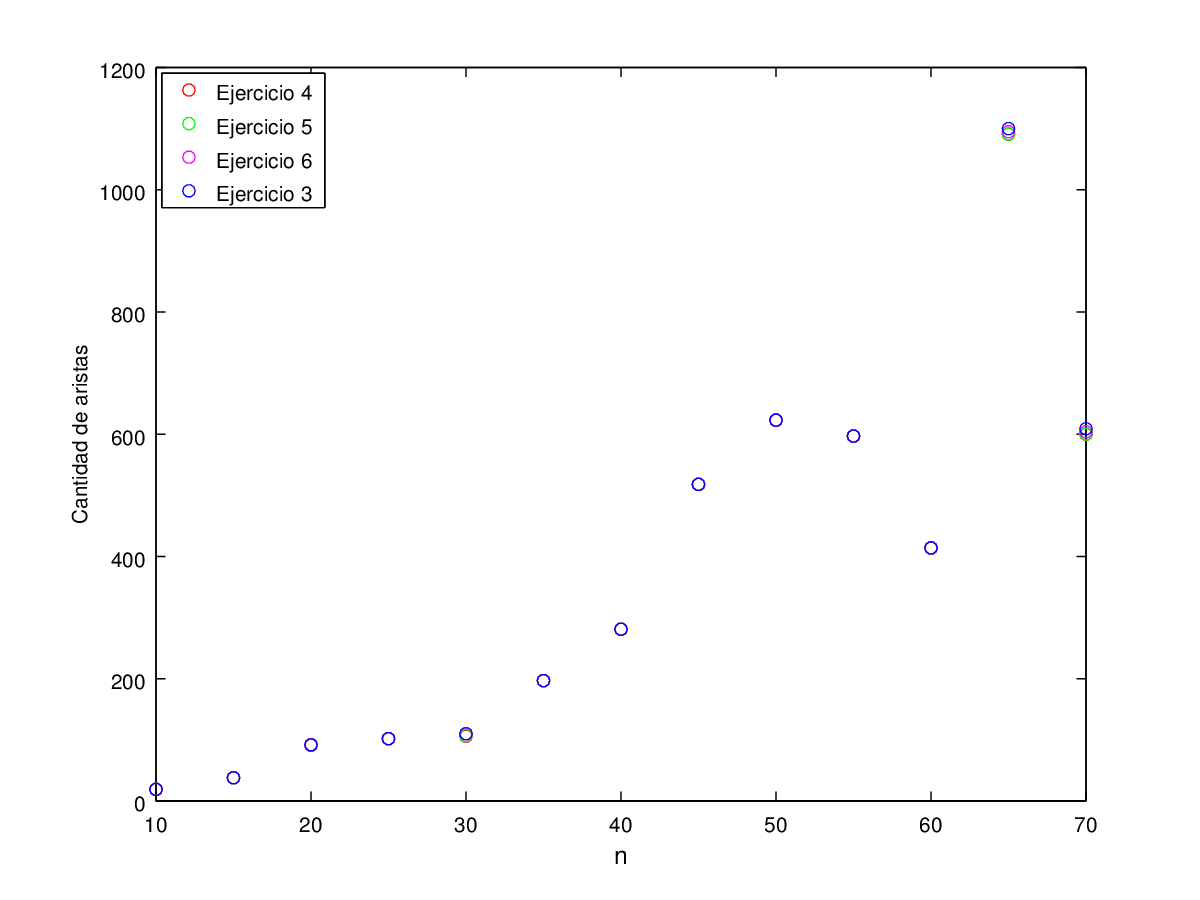
\includegraphics[height=10cm]{graficos/ejercicio7-exp4-comb1.png}
       \caption{Experimento 4- cografo y completo}
	\end{figure}
    
      \begin{figure}[H]
      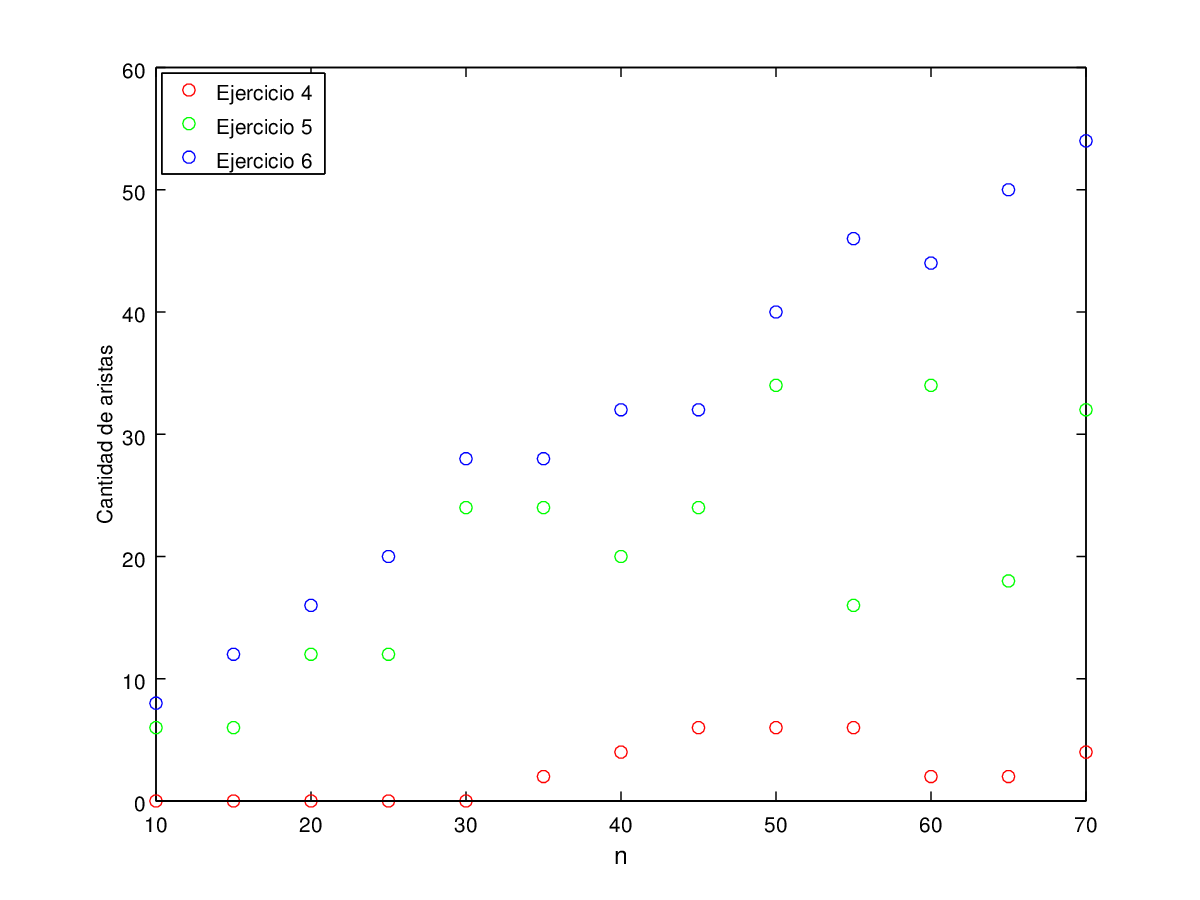
\includegraphics[height=10cm]{graficos/ejercicio7-exp4-comb2.png}
       \caption{Experimento 4- $C_n$ y bipartito completo}
	\end{figure}
    
      \begin{figure}[H]
      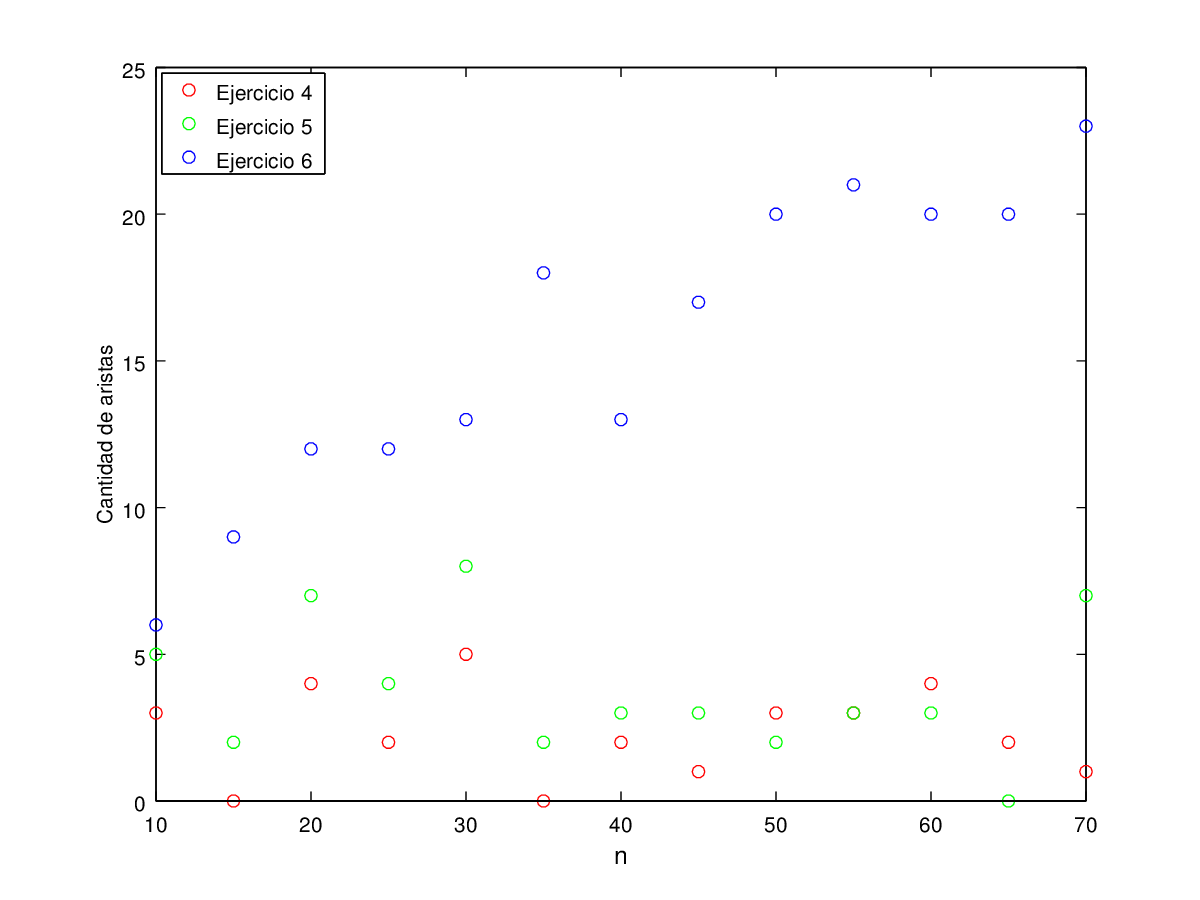
\includegraphics[height=10cm]{graficos/ejercicio7-exp4-comb3.png}
       \caption{Experimento 4- árbol y $C_n$}
	\end{figure}
    
    
    
\subsubsection*{Conclusiones}\;
En estos 3 grafos se observan diferentes comportamientos.\\
\begin{itemize}
\item En el primero que compara la cantidad de aristas de las solución de entre un cografo y un completo (las hip del Ej. 3), observamos que todos los algoritmos heurísticos son muy similares (cuando no iguales) al optimo, esto se lo atribuimos a que la heurística golosa es extremadamente eficaz en este caso particular, ya que el ordenar por grados y agarrar los vértices de mayor grado parece funcionar muy bien. Las otras 2 heurísticas parten del goloso y por lo tanto parten con una base muy solida para encontrar una mejor solución (El goloso en el peor caso mostró un margen de error respecto al optimo menor al 2\% para los casos probados).\\
En base a esto concluimos que si bien el mejor algoritmo para resolver este problema es exacto, pues encuentra la mejor solución y es el único que puede dar garantías, para entradas similares, por ejemplo, entre un cografo y un grafo casi completo o entre un grafo similar a un cografo y uno similar a un completo, incluso quizás entre uno relativamente con bastante aristas y uno casi completo, tendrá soluciones de una calidad aceptable, en un tiempo razonable, ya que podrá usar la metaheurística Tabú, o la búsqueda local si se quiere acortar los tiempos o incluso la heurística golosa que tiene un desempeño considerablemente mejor en tiempo de ejecución y aun así podría uno esperar en estos casos una solución de alta calidad.\\
\item En el segundo gráfico que se comparan los algoritmos heurísticos, ahora si sin un algoritmo exacto para comparar , ente un $C_n1$ y un $K_{n_2}$, se observa en este caso que la heurística golosa, contrariamente al caso anterior no es muy buena,en ningún caso encuentra mas de 10 aristas mientras que las otras heurísticas superan ampliamente ese numero (excepto en el caso n=10).\\
Se ve por otro lado que si bien la heurística goloso es mala, tanto la heurística de búsqueda local, como la metaheurística parecen ser considerablemente mejores y que la cantidad de aristas que encuentran en la solución es lineal en la cantidad de nodos(lo cual es bastante bueno, considerando que $C_n$ tiene $n$ aristas).\\
Considerando que si bien es notablemente mejor usar el algoritmo de heurística Tabú en esta situación si se quiere maximizar la cantidad de aristas, la decisión de utilizar este o el algoritmo de búsqueda local debe ser tomada considerando que el algoritmo de búsqueda local se ejecuta de manera mucho mas rápida.\\
Concluimos entonces que los mejores algoritmos para este tipo de instancias en particular, serán el de heurística Tabú, si lo que se quiere es encontrar la mejor solución posible o el de búsqueda local si lo que se quiere es una solución aceptable, pero que se ejecute en un periodo de tiempo mas corto.\\
No recomendamos para este tipo de instancia utilizar la heurística golosa ya que, si bien sera mas veloz en el tiempo de computo, la calidad de la solución es decir la cantidad de aristas, sera mucho mas baja.
\item En este último gráfico, se aprecia la experimentación rápidan de los algoritmos heurísticos ya mencionados entre un árbol y un $C_n$, tanto la heurística golosa como la heurística de búsqueda local, no parecen ser efectivas para encontrar una solución de calidad (al menos no de la calidad que encuentra la heurística Tabú).\\
En contraposición , la meta-heurística Tabú, si parece dar soluciones de calidad, ya que como notamos antes, la cantidad de aristas de la solución tiene un crecimiento lineal, lo que es mucho decir considerando que $C_n$ tiene $n$ aristas y un árbol de $n_2$ nodos tiene $n_2-1$ aristas.\\
Por lo tanto concluimos que si se quisiese resolver el problema con instancias de este tipo o similares, el algoritmo heurístico de Tabú es el mas recomendado a pesar de ser mas lento en cuanto a su tiempo de computo.\\
De necesitarse un algoritmo de resolución mas rápida, sugeriríamos plantear otra heurística golosa que se adapte mejor a la situación.\\
En caso que el tiempo se un factor decisivo y estemos obligados a elegir una de las 2 heurísticas mas veloces ya implementadas, la heurística golosa seria la indicada ya que la calidad de las soluciones sera baja en ambos casos pero el tiempo de computo sera sustancialmente mas corto.

\end{itemize}
Como conclusión general de  estas 3 instancias distintas del problema, observamos que cada una de las 3 heurísticas puede ser mas conveniente en distintos escenarios, esta en el análisis, la experimentación y el conocimiento del contexto de uso así como de las limitaciones y requerimientos temporales el cual es la mejor opción a elegir.
\clearpage


\end{document}